\RequirePackage{fix-cm}
\RequirePackage{amsmath}
\documentclass[smallextended]{svjour3}
\smartqed 
\usepackage{balance}
\usepackage{colortbl}
\usepackage{graphicx}
\usepackage{lscape}
\usepackage{multirow}
\usepackage{tcolorbox}
\usepackage{url}
\usepackage{xspace}

\usepackage{tikz}
\usetikzlibrary{automata,arrows,positioning,calc}
\everymath{\displaystyle}

\usepackage{pgfplots}
\pgfplotsset{compat=1.15}

% \usepackage{comment}
% \usepackage{fancybox}
% \usepackage{hyperref}
%\usepackage{mathtools}
% \usepackage{pdflscape}
% \usepackage{subfigure}

% ------------------------------------------------------------------------------
\newcommand{\hypobox}[1]{\begin{center}%
   \noindent\thicklines\setlength{\fboxsep}{8pt}%
    \cornersize{0.2}\Ovalbox{\begin{minipage}{3.0in}%
        \textit{#1}\end{minipage}} \end{center}}
% -----------------------------------------------------------------------------

\renewcommand{\paragraph}[1]{\noindent\textbf{\textsf{#1}:}}

\newcommand{\ie}{\emph{i.e.,}\xspace}
\newcommand{\eg}{\emph{e.g.,}\xspace}
\newcommand{\etc}{\emph{etc.}\xspace}
\newcommand{\etal}{\emph{et al.}\xspace}

%\newcommand{\foutse}[1]{\textcolor{blue}{{\it [Foutse says: #1]}}}
%\newcommand{\Saidur}[1]{\textcolor{green}{{\it [SR: #1]}}}
%\newcommand{\Azadeh}[1]{\textcolor{orange}{{\it [AZ: #1]}}}
%\newcommand{\TODO}[1]{\textcolor{cyan}{{\it [TODO: #1]}}}
%\newcommand{\newtext}[1]{\textcolor{purple}{{[#1]}}}
%\newcommand{\YANN}[1]{\textcolor{cyan}{{\it [YANN: #1]}}}

\newcommand{\RQOne}{Do design patterns and--or design anti-patterns mutate during software evolution and what is the probability of the mutations?}

\newcommand{\RQTwo}{What types of changes lead to  mutations between design patterns and design anti-patterns?}

\newcommand{\RQThree}{What is the fault-proneness of mutated design patterns and anti-patterns and what transitions lead to more fault-prone mutations?}

\newcommand{\RQFour}{Do specific types of changes lead to increased fault-proneness during mutations?}



\begin{document}

\title{Investigating Design Anti-pattern and Design Pattern Mutations and Their Change- and Fault-proneness}

\titlerunning{Design Anti-pattern and Design Pattern Mutations}

\author{Zeinab (Azadeh) Kermansaravi \and
        Md Saidur Rahman \and
        Foutse Khomh 		\and
        Fehmi Jaafar \and
        Yann-Ga\"{e}l Gu\'{e}h\'{e}neuc
}
\institute{Zeinab Kermansaravi \at
            SWAT Lab, Ptidej Team, DGIGL, Polytechnique Montr\'{e}al, Montr\'{e}al, QC, Canada\\
		    \email{zeinab.kermansaravi@polymtl.ca}
	    \and
 		    Md Saidur Rahman \at
            SWAT Lab, DGIGL, Polytechnique Montr\'{e}al, Montr\'{e}al, QC, Canada\\
            \email{saidur.rahman@polymtl.ca}
    	\and
 		    Foutse Khomh \at
            SWAT Lab, DGIGL, Polytechnique Montr\'{e}al, Montr\'{e}al, QC, Canada\\
           	\email{foutse.khomh@polymtl.ca}
        \and
	    	Fehmi Jaafar \at
            Computer Research Institute of Montr\'{e}al, Montr\'{e}al, QC, Canada\\
            \email{fehmi.jaafar@crim.ca}
        \and	
            Yann-Ga\"{e}l Gu\'{e}h\'{e}neuc \at
            Ptidej Team, CSSE, Concordia University, Montr\'{e}al, QC, Canada\\
            \email{yann-gael.gueheneuc@concordia.ca}
}
\date{Received: date / Accepted: date}
\maketitle

\begin{abstract}
During software evolution, inexperienced developers may introduce design anti-patterns when they modify their software systems to fix bugs or to add new functionalities based on changes in requirements. Developers may also use design patterns to promote software quality or as a possible cure for some design anti-patterns. Thus, design patterns and design anti-patterns are introduced, removed, and mutated from one another by developers.

Many studies investigated the evolution of design patterns and design anti-patterns and their impact on software development. However, they investigated design patterns or design anti-patterns in isolation and did not consider their mutations and the impact of these mutations on software quality. Therefore, we report our study of bidirectional mutations between design patterns and design anti-patterns and the impacts of these mutations on software change- and fault-proneness. 

We analyzed snapshots of seven Java software systems with diverse sizes, evolution histories, and application domains. We built Markov models to capture the probability of occurrences of the different design patterns and design anti-patterns mutations. Results from our study show that (1) design patterns and design anti-patterns mutate into other design patterns and--or design anti-patterns. They also show that (2) some change types primarily trigger mutations of design patterns and design anti-patterns (renaming and changes to comments, declarations, and operators), and (3) some mutations of design anti-patterns and design patterns are  more faulty in specific contexts.

These results provide important insights into the evolution of design patterns and design anti-patterns and its impact on the change- and fault-proneness of software systems.

\keywords{Design smells \and Design patterns \and Anti-patterns \and Fault-proneness \and Change-proneness \and Markov Chain}
\end{abstract}

\section{Introduction}
\label{sec:Introduction}


The goal in top-$\size$ recommendation is to recommend to each
consumer a small set of $\size$ items from a large collection of
items~\cite{cremonesi2010performance}.  For example, Netflix may want
to recommend $\size$ appealing movies to each consumer.  Collaborative
Filtering (CF)~\cite{herlocker2002empirical,lee2012comparative} is a
common top-$\size$ recommendation method.  CF infers user interests by
analyzing partially observed user-item interaction data, such as user
ratings on movies or historical purchase
logs~\cite{kanagal2012supercharging}. The main assumption in CF is that
users with similar interaction patterns have similar interests.


Standard CF methods for top-$\size$ recommendation focus on making  suggestions  that accurately reflect the user's preference history. However, as  observed in previous work,  CF recommendations are generally biased toward  popular items, leading to a rich get richer effect~\cite{vargas2014improving,steck2011item}.  The major reasons for this are \textit{popularity bias} and \textit{sparsity} of CF interaction data (detailed in Section~\ref{sec:related-work}). In a nutshell, to maintain  accuracy, recommendations are generated from the dense regions of the data,  where the popular items lie.  

However,  accurately suggesting popular items, may not be satisfactory for the consumers. For example, in Netflix, an accuracy-focused movie recommender may recommend ``Star Wars: The Force Awakens'' to users who have seen ``Star Wars: Rogue One''.  But, those users are probably already aware of ``The Force Awakens''. Considering additional factors, such as novelty of recommendations,  can lead to more effective suggestions~\cite{cremonesi2010performance,Castells2015,zhang2008avoiding,ziegler2005improving,zhang2012auralist}. 
%Second, accuracy-focused models typically achieve a   overall item-space coverage across their recommendations,  whereas high item-space coverage helps providers of the items increase revenue
%, users satisfaction since they are  likely already aware of or can find these items on their own.  

Focusing on popular items also adversely affects the satisfaction of  the providers of the items. This is because  accuracy-focused models typically achieve a  low overall item space coverage across their recommendations, whereas   high item space coverage helps providers of the items increase their revenue~\cite{vargas2014improving,Castells2015,adomavicius2011maximizing,anderson2006thelongtail, yin2012challenging,adomavicius2012improving}.
%accuracy-focused models typically achieve a

In contrast to the relatively small number of popular items, there are copious  {\it long-tail\/} items that have fewer observations (e.g., ratings) available. More precisely,  using the Pareto  principle (i.e.,~the $80/20$ rule),  long-tail items can be defined as items that generate the lower $20\%$ of observations~\cite{yin2012challenging}. Experimentally we found that these items correspond to almost $85\%$ of the items in several datasets (Sections~\ref{sec:Notation} and \ref{sec:Experiments}). %Table~\ref{tab:DatasetStatsticsSmall})


As previously shown, one way to improve the novelty of top-$\size$ sets is to recommend interesting long-tail items~\cite{cremonesi2010performance,ge2010beyond}.  The intuition  is that since they have fewer observations available,  they are more likely to be unseen~\cite{Kaminskas:2016:DSN:3028254.2926720}.  
 %For example, in online commerce,  newly added items are long-tail items that are yet to be discovered.  
Moreover, long-tail item promotion also results in higher overall coverage of the item space%, which increases profits for providers of the items
~\cite{vargas2014improving,Castells2015,zhang2008avoiding,zhang2012auralist,adomavicius2011maximizing,anderson2006thelongtail,yin2012challenging,jambor2010optimizing}. Because long-tail promotion reduces accuracy~\cite{steck2011item}, there are trade-offs to be explored.


%original submitted to ICDE
%This work studies three aspects of top-$\size$ recommendation: accuracy, novelty, and item-space coverage, and examines their trade-offs. In most previous work, predictions of a base recommendation system are re-ranked to handle their trade-offs~\cite{adomavicius2012improving,jambor2010optimizing,zhang2013personalize,wang2009portfolio}. Due to performance considerations, however, these techniques are not customized per user. For example,  parameters that balance the trade-off between novelty and accuracy are cross-validated at a global level.  This can be detrimental since users have varying preferences for  objectives such as long-tail novelty. We explore how to  automatically infer  user  preference for long-tail novelty, and how to leverage  it to correct  the popularity bias in standard recommender models. Our work does not rely on any additional contextual data, although such data, if available, can help promote newly-added long-tail items~\cite{agarwal2009regression,Saveski:2014:ICR:2645710.2645751}.

This work studies three aspects of top-$\size$ recommendation: accuracy, novelty, and item space coverage, and examines their trade-offs. In most previous work, predictions of a base recommendation algorithm are \textit{re-ranked} to handle these trade-offs~\cite{adomavicius2012improving,jambor2010optimizing,zhang2013personalize,wang2009portfolio}. The re-ranking models are computationally efficient but suffer from two drawbacks. First, due to performance considerations,  parameters that balance the trade-off between novelty and accuracy  are not customized per user. Instead they are cross-validated at a global level.  This can be detrimental since users have varying preferences for  objectives such as long-tail novelty. Second,  the re-ranking methods are often limited to a specific base recommender  that may be sensitive to dataset density. 
As a result, the datasets are pruned and the problem is studied in dense settings~\cite{adomavicius2012improving,ho2014likes}; but real world  scenarios are often sparse~\cite{kanagal2012supercharging,liu2017experimental}.   
% Because  dataset density can impact the performance of most base recommenders (like R-SVD), which in turn affects the performance of the re-ranking model, 

\iffalse
We address these limitations by directly inferring  user  preference for long-tail novelty  from interaction data.  This  allows us to customize the re-ranking  per user, and design a \textit{generic} framework, which resolves the second problem. In particular, since the long-tail novelty preferences are estimated independently of any base  recommender model, we can  plug-in an appropriate base recommender w.r.t. the dataset sparsity.% including ones that are more suitable for sparse settings.  

Modelling  user  preference for  long-tail novelty using only item popularity statistics, e.g., the average popularity of rated items as in~\cite{jugovac2017efficient}, disregards additional information like whether the user found the item interesting and the long-tail preferences of other users  of the items. \iffalse To incorporate them, we introduce the notion of  \emph{item long-tail importance}. Both  user long-tail preferences and item long-tail importance are dependent:  a user has high preference for discovering long-tail items if she is interested in important long-tail items, and an item that is associated with many of these kinds of users is likely to be more important.  We propose a joint optimization framework to directly learn,  from interaction data, both the users' long-tail preferences and the  items' long-tail importance. \fi
We propose an optimization approach that  incorporates  this information and  directly learns,  from interaction data, the users' long-tail novelty preferences.

Next, we use these learned preferences  to design a  top-$\size$ recommendation framework thats is generic, and provides customized balance between accuracy, novelty, and coverage. We refer to it as framework as GANC.  Using GANC, we design a novel algorithm, {\it Ordered Sampling-based Locally Greedy (OSLG)\/}, that relies on the learned long-tail novelty preferences  to scalably correct for popularity bias. Our work does not rely on any additional contextual data, although such data, if available, can help promote newly-added long-tail items~\cite{agarwal2009regression,Saveski:2014:ICR:2645710.2645751}. In summary:
\fi

We address the first limitation by directly inferring  user  preference for long-tail novelty  from interaction data.   Estimating these  preferences  using only item popularity statistics, e.g., the average popularity of rated items as in~\cite{jugovac2017efficient}, disregards additional information, like whether the user found the item interesting or the long-tail preferences of other users  of the items. We propose an approach that  incorporates  this information and  learns the users' long-tail novelty preferences from interaction data.

This approach allows us to customize the re-ranking  per user, and  design a \textit{generic} re-ranking framework, which resolves the second limitation of prior work. In particular, since the long-tail novelty preferences are estimated independently of any base recommender, we can  plug-in an appropriate one w.r.t. different factors, such as the dataset sparsity.

Our top-$\size$ recommendation framework, \textbf{GANC}, is \textbf{G}eneric, and provides customized balance between \textbf{A}ccuracy, \textbf{N}ovelty, and \textbf{C}overage. % Moreover, based on the learned long-tail novelty preferences, we also design a novel algorithm, {\it Ordered Sampling-based Locally Greedy (OSLG)\/}, that relies on the learned long-tail novelty preferences  to scalably correct for popularity bias. 
Our work does not rely on any additional contextual data, although such data, if available, can help promote newly-added long-tail items~\cite{agarwal2009regression,Saveski:2014:ICR:2645710.2645751}. In summary:

%Consider  the following toy example:
\vspace{-0.2cm}
\begin{table}[htb]
\centering
\scriptsize
%\small
\begin{tabular}{ccccccc} 
%\toprule
%&\multirow{2}{*}{}&\multicolumn{7}{c}{Ratings}\\
& & \cellcolor{blue!35}$w_1$ &\cellcolor{blue!18} $w_2$ & $\dots$ &\cellcolor{blue!8} $w_{89}$  &\cellcolor{blue!8} $w_{99}$   
\\
&   &$i_1$&$i_2$&$\dots$&$i_{89}$&$i_{90}$\\ 
\cmidrule(r){3-7} 	 
%\midrule
\cellcolor{red!35}$\theta_1$  &$u_1 $   &5 &   & $\dots$ &  &   \\
\cellcolor{red!28}$\theta_2$  &$u_2$     &5 &    & $\dots$ &  &  \\
 $\theta_3=?$  &$\bf u_3$  &5 &  &   $\dots$ &  &  \\
\cellcolor{red!10}$\theta_4$ & $u_4$  &  &5   & $\dots$ & &\\ 
\cellcolor{red!10}$\theta_5$ & $u_5$  &  & 5  & $\dots$ & &\\ 
$\theta_6=?$  & $\bf u_6$ & &5  &      $\dots$& &  \\ 
 & & $\hdots$  &$\hdots$   &$\hdots$   &$\hdots$   &$\hdots$  \\
%\midrule 
\cmidrule(r){3-7} 	 
\multicolumn{2}{c}{item pop.}  & 3  & 3  & $\dots$ &50&60\\  
%\bottomrule
%$ f_i$    &3  &3  &1  &3  &1  &2  \\  \hline
\end{tabular}
%#.
\caption{Simplified user-item interaction data. The user long-tail novelty preference ($\theta_u$), item long-tail importance weight ($w_i$) are highlighted. Darker colors indicate larger values. } \label{tab:example}
\end{table} 
\vspace{-0.2cm}
\begin{example}  
In Table~\ref{tab:example}, we are interested in estimating $\theta_3$ and $\theta_6$,  the long-tail preference of users $u_3$ and $u_6$ who have each rated a single movie. Additional ratings for other users  are not included here.  Considering only rating information, we observe $i_1$ and $i_2$ are  equally popular $|\mathcal{U}_{i_1}^{\trainset}| = |\mathcal{U}_{i_2}^{\trainset}|=3$, and $r_{31}=5$ and $r_{62}=5$. Using Eq.~\ref{eq:tfidf-risk}  we have $\theta_3 = \theta_6$. However, if we were given the long-tail preferences of the each item's user set, specifically that $u_1$ and $u_2$ have high long-tail preference (darker red), while $u_4$ and $u_5$ have lower long-tail preference (lighter red), we could conclude $i_1$ is a more important long-tail item compared to $i_2$ (indicated by a darker blue shade for $w_1$), and we expect  $\theta_3 \geq \theta_6$.

% On the other hand, if we knew that $u_4$ and $u_5$ have lower long-tail preference, we could conclude $i_2$ is a  less significant long-tail item. Therefore, However, if we  consider the long-tail preferences of other users, we may reason differently.    We need another variable $w_i$ which captures this information. 
%we would conclude that $u_3$ has higher long-tail preference compared to $u_6$, since the users $i_1$ is a more prominent long-tail item. 

% Relying only  on item popularity information, we would  conclude   $u_3$ and $u_6$ have equal long-tail preference, since $i_1$ and $i_2$ are  equally popular. However, considering  the second column,  long-tail preference of users,  long-tail importance for each item,  which captures the long-tail preference of its users. Since  that  both users of $i_1$ have high long-tail preference while  the users of $i_2$ have lower preference,  we may conclude $i_1$ is a more important long-tail item compared to $i_2$. Therefore, $u_3$'s long-tail preference should be at least as large as $u_6$'s preference. Specifically, consider two  items $i_1$ and $i_2$, with the following rating data: $i_1=\{u_1:5, u_2:5, u_3:5 \}$, $i_2=\{u_4:5, u_5:5, u_6:5\}$.  

%Table~\ref{tab:example} shows  simplified rating data. We want an estimate of the long-tail preference of $u_3$ and $u_6$, who have each  rated a single movie.  Relying only  on movie popularity information, we would  conclude   $u_3$ and $u_6$ have similar long-tail preference, since $m_1$ and $m_2$ are  equally popular. However, considering the long-tail preferences of other users of those movies, we may reason differently: since $u_1$ and $u_2$ have high long-tail preference, and $u_4$ and $u_5$ have low long-tail preference, $m_1$ is a more prominent long-tail item compared to $m_2$. Therefore, it is likely that $u_3$ has higher long-tail preference compared to $u_6$.considering the long-tail preferences of other users of those movies, we may reason differently.  For example, 
\label{ex:running}
\end{example}



%------------------------------

\iffalse
\begin{example}
Table~\ref{tab:example} shows rating data for a simplified system. %Note the user-item interaction matrix is sparse.
For this example, we define popular movies as those that have received  three or more ratings; $\{m_1, m_2, m_4\}$ are popular and  $\{m_3, m_5, m_6\}$ are niche movies. We observe $u_1$ and $u_3$  have rated relatively popular movies (risk-averse) while $u_2$ and $u_4$ have rated niche movies (risk-loving). 
\label{ex:running}
\end{example}

\begin{table}[htb]
\centering
\scriptsize
\begin{tabular}{ccccccc} 
\toprule
			&$m_1$ &$m_2$   &$m_3$    &$m_4$   &$m_5$ &$m_6$  \\ \hline 
$u_1 $ &5  &4  & - &-  &-  &-   \\
$u_2$  &-  &-  &-  &-  &5  &5   \\
$u_3$  &-  &4  &-  &5  &-  &-   \\
$u_4$  &-  &-  &3  &-  &-  &4   \\ 
$u_5$  &5  &-  &-  &3  &-  &-   \\ 
$u_6$  &4  &2  &-  &4  &-  &-   \\ 
\bottomrule
%$ f_i$    &3  &3  &1  &3  &1  &2  \\  \hline
\end{tabular}
\caption{User-Movie rating data} \label{tab:example}
\end{table}

It is essential to consider consumer characteristics in designing recommender systems so that they promote long-tail items to the right group of users and spread demand evenly between hit and niche items.  

\fi





%------------------------------
\iffalse
\begin{table}[htb]
\centering
\scriptsize
\begin{tabular}{ccccccc} 
\toprule
			&$m_1$ &$m_2$   &$m_3$    &$m_4$   &$m_5$ &$m_6$  \\ \hline 
$u_1 $ &\textbf{5}  & \textbf{4}  &\textcolor{gray}{ 1.2} &-  &-  &-   \\
$u_2$  &-  &-  &-  &-  & \textbf{5}  &\textbf{5}   \\
$u_3$  &-  &\textbf{4}  &-  &\textbf{5}  &-  &-   \\
$u_4$  &-  &-  &\textbf{3}  &-  &-  &\textbf{4}   \\ 
$u_5$  &\textbf{5}  &-  &-  &\textbf{3}  &-  &-   \\ 
$u_6$  &\textbf{4}  &\textbf{2}  &-  &\textbf{4}  &-  &-   \\ 
\bottomrule
%$ f_i$    &3  &3  &1  &3  &1  &2  \\  \hline
\end{tabular}
\caption{User-Movie rating data} \label{tab:example}
\end{table}
% $\mathcal{P}^1= \{ \mathcal{P}_1^1 \{i_1,i_2,i_3\}, \mathcal{P}_2^1:\{i_2,i_3,i_5\}  \}$
 %$\mathcal{P}^2= \{ \mathcal{P}_1^2: \{i_1,i_2,i_3\}, \mathcal{P}_2^2:\{i_2,i_5,i_6\}  \}$
 %$\mathcal{P}^3= \{ \mathcal{P}_1^3: \{i_7,i_8,i_9\}, \mathcal{P}_2^3:\{i_{10},i_{11},i_{12}\}  \}$
\begin{table}[htb]
\centering
\tiny
\begin{tabular}{ccc} 
\toprule
		&$u_1$&$u_2$  \\ \hline 
$\mathcal{P}^1 $ & $\{i_1,i_2,i_3\}$ & $\{i_2,i_3,i_5\} $ \\
$\mathcal{P}^2$ & $\{i_1,i_2,i_3\}$ & $\{i_2,i_5,i_6\} $ \\
$\mathcal{P}^3$ & $\{i_7,i_8,i_9\}$ & $\{i_{10},i_{11},i_{12} \}$ \\
\bottomrule
%$ f_i$    &3  &3  &1  &3  &1  &2  \\  \hline
\end{tabular}
\caption{Top-$\size$ allocations to users.} \label{tab:paretoExamples}
\end{table}
\fi


\iffalse
When considering long-tail items, it is important to consider consumers' willingness  to explore niche or unpopular items and their propensity towards similar items. In particular, they can be characterized by their  {\it risk degree\/} and {\it focusing degree\/}, respectively.  We compute these estimates  based on historical rating information. The following example further describes these notions in the context of movie rating data. 

\begin{example}  
Table~\ref{tab:example} shows rating data for a simplified system with $6$ users, $6$ movies, and $3$ genres. $m_i^{j}$ implies that movie $m_i$ belongs to genre $j$. Note the user-item interaction matrix is sparse. 
  For this setting, we define popular movies as those that have received  three or more ratings; $\{m_1, m_2, m_4\}$ are popular and  $\{m_3, m_5, m_6\}$ are niche movies. We now profile the users according to their risk and focusing degree. E.g., $u_1$ has rated relatively popular movies belonging to the same genre (risk-averse, high focusing degree); $u_2$ has rated niches movies in the same genre (risk-loving, high focusing degree); $u_3$ has rated popular movies in two different genres (risk-averse, low focusing degree), and $u_4$ has rated niches movies in two different genres (risk-loving, low focusing degree). 
\label{ex:running}
\end{example}
\begin{table}[htb]
\centering
\tiny
\begin{tabular}{ccccccc} 
\toprule
			&$m_1^{1}$ &$m_2^{1}$   &$m_3^{2}$    &$m_4^{3}$   &$m_5^{3}$ &$m_6^{3}$  \\ \hline 
$u_1 $ &5  &4  &-  &-  &-  &-   \\
$u_2$  &-  &-  &-  &-  &5  &5   \\
$u_3$  &-  &4  &-  &5  &-  &-   \\
$u_4$  &-  &-  &3  &-  &-  &4   \\ 
$u_5$  &5  &-  &-  &3  &-  &-   \\ 
$u_6$  &4  &2  &-  &4  &-  &-   \\ 
\bottomrule
%$ f_i$    &3  &3  &1  &3  &1  &2  \\  \hline
\end{tabular}
\caption{User-Movie rating data} \label{tab:example}
\end{table}
It is essential to consider these consumer characteristics in designing recommender systems so that they promote long-tail items to the right group of users and spread demand evenly between the hit and niche items.  
\fi
\iffalse
\begin{center}
\begin{figure*}[tp]
%\scalebox{0.5}{%
\resizebox{1\textwidth}{!}{%
%\small%\addtolength{\tabcolsep}{5pt}% below sums to 8
\begin{tabularx}{1.5\textwidth}{>{\hsize=2.5\hsize}X>{\hsize=2.5\hsize}X>{\hsize=0.5\hsize}X>{\hsize=0.5\hsize}X>{\hsize=0.5\hsize}X>{\hsize=0.5\hsize}X>{\hsize=0.5\hsize}X>{\hsize=0.5\hsize}X}
    \multirow{12}{*}{\includegraphics[scale=0.3]{codeForExample/popularity-movie.png}} & \multirow{12}{*}{\includegraphics[scale=0.3]{codeForExample/scatterplot.png}} & & & & & & \\
%   & &               &       &       &       &       &       \\
    & &\multicolumn{1}{l|}{}               &$m_1^{g1}$   	&$m_2^{g1}$    	&$m_3^{g2}$    &$m_4^{g2}$      &$m_5^{g3}$    \\ \cline{3-8}%\hline
    & &\multicolumn{1}{l|}{u1}          &5  &5  &-  &-   &-  \\
    & &\multicolumn{1}{l|}{u2}    		&-  &-  &4  &4  &5  \\
    & &\multicolumn{1}{l|}{u3}   			&1  &2  &1  &-  &-   \\
    & &\multicolumn{1}{l|}{u4}     		&1  &-  &-  &-  &-  \\
    & &               &       &       &       &       &       \\
    & &               &       &       &       &       &       \\
    & &               &       &       &       &       &       \\
    & &               &       &       &       &       &	\\
    \\
\end{tabularx}}
\caption{User-Movie interaction data a) Popularity-Movie histogram b)Movie genres/clusters c) User-Movie rating data} \label{fig:example}
\end{figure*}
\end{center}
\fi



%We propose a novel approach that allows us to  promote long-tail items in a targeted manner, thereby improving the novelty of top-$\size$ sets, the overall item-space coverage across recommendations, while maintaining reasonable levels of accuracy.

%Next, we integrate these learned preferences  in a generic  top-$\size$ recommendation framework to provide customized balance between accuracy and coverage.

%sequentially make recommendations, while adjusting its parameters with regard to the set of top-$\size$ recommendations made so far. However, since  sequential parameter updates  cause  scalability issues, we propose a sampling based algorithm. This variant of our framework, called {\it Ordered Sampling-based Locally Greedy (OSLG)\/},  allows us to  correct for the popularity bias in recommendations with regard to individual user long-tail preferences. 

%ICDE submission
%Our framework differs with  prior work in the following aspects:  unlike~\cite{adomavicius2011maximizing,adomavicius2012improving,zhang2013personalize,ho2014likes},  the long-tail preference personalization in our framework is learned rather than optimized using cross-validation or parameter tuning. In other words, our personalization method is independent of the underlying base  recommendation models.  Moreover, our framework is  generic. This enables us to  plug-in several base recommenders, and evaluate their  effectiveness without requiring  extensive tuning for the accuracy and coverage trade-off. 


%\vspace{-2.8pt}
\begin{itemize}

\item  We examine various measures for estimating user long-tail novelty preference in Section~\ref{sec:lt-pref} and formulate an optimization problem  to directly learn users' preferences for long-tail  items from interaction data in Section~\ref{sec:learning-lt-pref}. %In addition, we introduce several heuristics for measuring the user preference for less common items from historical rating data.% 

\item  We integrate the user preference estimates into GANC %, a generic re-ranking framework that provides customized balance between accuracy, novelty, and coverage 
(Section~\ref{sec:RiskbasedReranking}), and  introduce {\it Ordered Sampling-based Locally Greedy (OSLG)\/}, a scalable algorithm that relies  on user long-tail preferences to correct the popularity bias (Section~\ref{sec:optimizationAlgorithm}).
%We introduce OSLG, a scalable algorithm that relies  on user long-tail preferences to  maximize item space coverage \textcolor{red}{while maintaining acceptable levels of accuracy} (Section~\ref{sec:optimizationAlgorithm}).

\item   We conduct an extensive empirical study and evaluate performance from  accuracy, novelty, and coverage perspectives (Section~\ref{sec:Experiments}).  We use five  datasets with varying density and difficulty levels. %:  Netflix, MovieTweetings, and MovieLens (100K, 1M, 10M). 
  In contrast to most related work,  our evaluation considers realistic settings that include a large number of infrequent  items and users. %This enables us to study the impact of  data density on the performance trade-offs of several  state of the art top-$\size$ recommendation algorithms. %   %,  and use the all-items ranking protocol~\cite{steck2013evaluation,vargas2014improving}, where performance is measured using all items with train data. to evaluate the performance of several  state of the art top-$\size$ recommendation algorithms 
 
\item Our empirical results confirm that the performance of re-ranking models is impacted by the underlying   base recommender and the dataset density. Our generic approach enables us to easily incorporate a suitable base recommender to devise an effective solution for both dense and sparse settings. In dense settings, we use the same base recommender as existing re-ranking approaches, and we outperform them in accuracy and coverage metrics. For sparse settings, we plug-in a more suitable base recommender, and devise an effective solution that is competitive with existing top-$\size$ recommendation methods in accuracy and novelty. 

%Directly estimating the long-tail novelty preferences allows us to customize re-ranking per user, and  devise a generic framework.   
 
\end{itemize}

Section~\ref{sec:related-work} describes related work. Section~\ref{sec:conclusion} concludes.

\section{Related Work}
\label{sec: Related Work}
In this section, we introduce two representative diversity estimators and discuss the difficulties they meet when handling MMOPs. Subsequently, some existing multi-modal multi-objective optimization algorithms are reviewed.
\subsection{Review of diversity estimators}
\subsubsection{Density in SPEA2}
In SPEA2 \cite{SPEA2}, each solution is assigned a density value which is used to calculate its fitness value. Eq. (\ref{eq: Density in SPEA2}) gives the density of a solution $\boldsymbol{x}$.
\begin{equation}
	\textit{Density} (\boldsymbol{x}) = \frac{1}{\sigma_k(\boldsymbol{x}) + 2},
	\label{eq: Density in SPEA2}
\end{equation}
where $\sigma_k(\boldsymbol{x})$ is the distance from $\boldsymbol{x}$ to its $k$-th nearest neighbor in the objective space. In SPEA2, $k$ is set to the square root of the total number of solutions in the current population as a general parameter setting.

Notice that in SPEA2, higher density means worse diversity in the objective space.

\subsubsection{Crowding distance}
Crowding distance is proposed along with the NSGA-II algorithm\cite{NSGAII} to preserve the diversity of the population in the objective space. The crowding distance of a solution $\boldsymbol{x}$ is given by the average side length of the hypercube constructed by its left and right neighbors in each objective. More precisely, for each objective, the left and right neighbors of $\boldsymbol{x}$ are the solutions at the left and right positions of $\boldsymbol{x}$ for that objective (i.e., in the list obtained by sorting the population in an increasing order of the objective values of that objective). The crowding distance of all boundary solutions (i.e., best solutions in any objectives) are set to $\infty$ to ensure that they are always selected. In NSGA-II, larger crowding distance values indicate better diversity. Formally, Eq. (\ref{eq: crowding distance}) calculates the crowding distance for a solution $\boldsymbol{x}$.
\begin{equation}
	\textit{Crowding-Distance} (\boldsymbol{x}) =
	\begin{cases}
		\infty                                                                     & ,\boldsymbol{x} \text{ is a boundary solution} \\
		\frac{1}{M}\sum_{m=1}^M[f_m(\boldsymbol{x}_{rm})-f_m(\boldsymbol{x}_{lm})] & ,\text{otherwise}
	\end{cases},
	\label{eq: crowding distance}
\end{equation}
where $M$ refers to the number of objectives, and $\boldsymbol{x}_{lm}$ and $\boldsymbol{x}_{rm}$ are the left and right neighbors of solution $\boldsymbol{x}$ regarding the $m$-th objective, respectively.
\subsection{Difficulties when handling MMOPs}
In most diversity estimators in MOEAs, the solution distribution in the decision space is out of consideration, which makes them inefficient on MMOPs. As we have discussed in Section \ref{sec: Introduction}, in MMOPs, equivalent solutions have the same or almost the same objective values. Consequently, they are usually not preferable in terms of diversity (in the objective space). For this reason, diversity estimators used in MOEAs are often responsible for the loss of equivalent solutions when tackling MMOPs. Fig. \ref{fig: Difficulty when handling MMOPs} gives an example when a diversity estimator such as crowding distance produces undesirable effects. In Fig. \ref{fig: Difficulty when handling MMOPs}, $A$ and $B$ are two Pareto optimal solutions on different (but equivalent) Pareto subsets (i.e., the upper and lower dash lines in (a)). Although $A$ and $B$ have similar objective values, the decision maker may want to keep both of them since they represent different implementations (i.e., they are different in the decision space). However, a diversity estimator tends to assign bad diversity values to them due to the small difference between their objective values. As a result, some of them are likely to be removed. From this example, we can see that solutions in different regions in the decision space should be considered separately when estimating solution diversity for MMOPs. Following this idea, we propose a niching diversity estimation method in Section \ref{sec: Proposed method}.

\begin{figure}
	\centering
	\includegraphics[width=.75\textwidth]{figures/RelatedWork/Difficulties}
	\caption{Explanation of the diversity loss in the decision space caused by diversity estimators when handling an MMOP. The dash lines in (a) and (b) denote the Pareto set and Pareto front, respectively.}
	\label{fig: Difficulty when handling MMOPs}
\end{figure}

\subsection{Multi-modal multi-objective optimization algorithms}
\label{sec: Existing multi-modal multi-objective optimization algorithms}
In most state-of-the-art multi-modal multi-objective evolutionary algorithms (MMEAs), the diversity in the decision space is maintained by niching strategies. Some MMEAs extend existing niching strategies in MOEAs to enable them to maintain the diversity in the objective space as well as in the decision space. For example, in \cite{OmniOptimizer}, Deb and Tiwari proposed one of the first MMEA called Omni-optimizer which modifies the crowding distance to measure the diversity in the decision space and the objective space simultaneously. Yue et. al. proposed a particle swarm optimizer named MO\_Ring\_PSO\_SCD \cite{MO_Ring_PSO_SCD} which adopts a similar modified crowding distance and a ring topology to create a niche structure. The DNEA algorithm \cite{DNEA} applies the fitness sharing \cite{Sharing} to both decision and objective spaces and combines them into a single sharing function. Some MMEAs are proposed with dedicated niching strategies in the decision space. Tanabe et. al. proposed a decomposition-based MMEA called MOEA/D-AD\cite{MOEAD_AD} where multiple solutions can be assigned to a weight vector, and a newly generated solution only competes with other solutions which are assigned to the same weight vector and neighboring to that solution in the decision space. In our previous study \cite{MOEAD_MM}, we proposed another decomposition-based MMEA which utilizes a clearing strategy in the decision space. Some MMEAs such as the algorithms proposed in \cite{DBSCAN_MMEA} and \cite{MMOEADC} use clustering approaches to maintain the niching structure in the decision space.
\section{Methodology}

% \begin{figure}[!t]
% \centering
% \includegraphics[width=\linewidth]{fig/FLDv3.pdf}
% \caption{Procedure of FLD}
% \label{Overview}
% \end{figure}

\begin{figure*}[!t]
\centering
\includegraphics[width=.8\linewidth]{fig/FLDv1.pdf}
\caption{Procedure of FLD}
\label{Overview}
\end{figure*}



\subsection{Motivation}
According to the attack analysis in constrain-and-scale~\cite{howtobackdoor}, the federated backdoor attacks are divided into two attack scenarios: single-shot attacks (\textit{Attack A-S}) and multi-shot attacks (\textit{Attack A-M})~\cite{xie2020dba,am1}.
\setlist[itemize]{leftmargin=*}
%\begin{itemize}

\noindent\textbf{\textit{Attack A-S}}: the attacker successfully embeds its backdoor trigger in only one round. The attacker performs parameter scaling on the compromised clients' updates to substitute the global model $G^{t}$ with a backdoor model $X$ in Equation~\ref{eq:backdooreq1}: 
\begin{equation}
\label{eq:backdooreq1}
X = {\sum_{i=1}^{n}} \frac{1}{n} w_{i}^{t}.
\end{equation}
To achieve this goal, the attacker can scale the model parameters as follows:
\begin{equation}
\begin{split}\label{eq:backdooreq2}
\tilde{w} _{n}^{t} 
& = nX-\sum_{i=1}^{n-1} w_{i}^{t}\approx nX-\sum_{i=1}^{n-1} G ^{t-1}\\
& = n\left ( X-G ^{t-1} \right )+G ^{t-1}.
\end{split}
\end{equation}
As the global model converges, $w_{i}^{t}\approx  G ^{t-1}$. In other words, the attacker scales up the model weights $X$ by $n$ to prevent the malicious updates from being mitigated by the aggregation.


\noindent\textbf{\textit{Attack A-M}} lets compromised clients accumulate malicious updates over multiple rounds, instead of directly scaling the uploaded parameters, to avoid being detected by the defense algorithm. 
%the malicious client does not scale the update, thus avoiding detection by the defence.The malicious clients are selected in multiple rounds thus accumulating malicious updates. 
%\end{itemize}
%After reviewing the backdoor defenses methods in FL, we found that the past defenses basically defaulted to the attacker performing \textit{Attack A-S} and ignoring \textit{Attack A-M}. However, after experiments, we found that the attacker can successfully embed the back model in the global model by using Attack A-M, and in this case, many defenses will fail, such as clipping, Euclidean distance, etc. 
We have thoroughly reviewed the SOTA backdoor defense works in federated learning~\cite{foolgold,krum,Trimmed_Mean,Bulyan,RFA,canyou} and found that existing methods focus on defending against \textit{Attack A-S} while overlooking \textit{Attack A-M}. Unsurprisingly, we found through empirical experiments that SOTA defense algorithms fail at defending against {\textit{Attack A-M}.
%\subsection{Overview}

To address the challenges mentioned above, we propose Federated Layer Detection~(FLD), an innovative defense method for effectively detecting backdoor attacks in federated learning that overcomes the deficiencies of previous works. As depicted in Fig.~\ref{Overview}, FLD consists of two components, namely Layer Scoring and Anomaly Detection. Layer Scoring assigns scores to the local models uploaded by the clients according to the concept of isolation. Anomaly Detection checks the outlier scores given by Layer Scoring to determine if an uploaded model is compromised. The overall process is as follows: 1) The server receives the local models from the clients participating in the current round. 2) The server assigns each layer of each model an outlier score using Layer Scoring. 3) The server labels each layer as abnormal or not according to its outlier score, and excludes from the aggregation the anomalous models that contain more anomalous layers than the predefined threshold, as summarized in Algorithm~\ref{algorithm1}.
\begin{algorithm}
    \caption{Overview}\label{algorithm1}
    \begin{algorithmic} [1]
        \algrenewcommand\algorithmicrequire{\textbf{Input:}}
        \Require Set of clients $ C = \left \{ C_{1},C_{2},C_{3},\cdots,C_{N}  \right \} $, local datasets $ D = \left \{ D_{1},D_{2},D_{3},\cdots,D_{N} \right \}$, the number of training iterations $T$, the percentage of participating clients per round $K$.
        \algrenewcommand\algorithmicrequire{\textbf{Output:}} 
        \Require Global model $G^T $
        \State Initialize the global model $G^0 $
        \For { $ t\ in \left [ 1,T \right ] $ }
        \State $ n\gets \max \left ( K\cdot N,1  \right ) $ 
        \State $ C^{t} \gets $ (random set of $n$ clients )
        \For {each client $ i\in C^{t} $ in parallel} 
        \State The server sends $G^{t-1}$ to client $i$
        \State $w_{i}^{t} \gets $ ClientUpdate$\left ( D_i, G^{t-1}  \right) $ 
        \State Client $i$ sends $w_{i}^{t}$ back to the server
        \EndFor
        \State $\left(S_{1} ,\cdots,S_{n}\right)\gets Layer Scoring\left(w_{1}^{t},\cdots,w_{n}^{t}\right)$
        \State $C_{b}^{t}\gets Anomaly Detection \left(S_{1} ,\cdots,S_{n}\right)$
        \State  $m\gets len\left ( C_b^t \right ) $
        \State  $  G^{t}=  \sum_{i\in  C_b}^{} \frac{1 }{m} w_{i}^{t}$
        \EndFor
    \end{algorithmic}
\end{algorithm}

%\subsection{Federated Layer Detection Design}

%
\subsection{Layer Scoring}
In round $t$, the parameter server sends the global model $G^{t-1}$ to the selected clients $i\in C^t$, each of which trains $G^{t-1} $ using its local data $D_{i}$ and sends the model parameters $w_{i}^{t}$ back to the server after local training is completed.
%Our aim is to eliminate the threat of potentially malicious local models.

Existing backdoor defense methods assess uploaded models based on either similarity or distance metrics. They usually flatten the parameters of each model layer and then stitch them into a vector to perform the assessment. However, different layers of the neural network have heterogeneous parameter value distribution spaces due to their different functions. For example, in a CNN, the lower layers learn to detect simple features such as stripes, the middle layers learn to detect a part of an object, and the higher layers learn to detect a concept (e.g., a person)~\cite{distribution}. As a result, directly flattening and splicing the parameters of each layer easily leads to the loss of important information and hence the escape of malicious models. Therefore, finer-grained detection is demanded.

To address this issue, we have devised a hierarchical detection method, Layer Scoring, to measure fine-grained model differences, as shown in Algorithm~\ref{algorithm2}. Layer Scoring examines and assigns an outlier score to each layer of the uploaded models in turn. To provide accurate scores, the outlier scoring method is crucial and faces the following challenges:
%The method , and for layer $j$, we use an outlier detection \textcolor{blue}{method} to detect layer $j$ of all uploaded models, assigning an anomaly score to each $j$ layer of each model. \textcolor{blue}{This outlier detection method faces two challenges:}

\noindent\textbf{C1}: \textbf{The proportion of compromised clients is unknown.} Many existing works on outlier detection reply to the impractical assumption of knowing the proportion of compromised clients in advance, which severely limits their applicability in reality. To address this limitation, in this work, we propose an algorithm without requiring such prior knowledge. As such, conventional outlier detection methods such as K-Nearest Neighbors (KNN) and One-Class SVM, which rely on prior knowledge of the number of neighbors, are not feasible. 

%Knowing the proportion of compromised clients is a common assumption in existing works which has a huge impact on their applicability in reality. In this work, we do not assume such knowledge. As a result, popular outlier detection methods such as KNN and ABOD which require the prior knowledge of the number of neighbors are not feasible.
%for the outlier detection method. For example, it is difficult to use commonly used algorithms such as KNN, LOF, etc., which require the number of neighbors to be specified in advance, or the choice of metric matrix, such as Euclidean distance or cosine distance, as we do not know the proportion of malicious attackers in advance.

\noindent\textbf{C2}: \textbf{Identifying backdoored models in dynamic scenarios.} In each round, the number of injected backdoors is unknown and may vary. Hence, it is important to have a stable backdoored model identification method that can effectively handle dynamic attacks. Otherwise, many false positives may be generated, failing the backdoor defenses and impacting the main task's accuracy.

% \textbf{C2}: \textbf{\textcolor{blue}{The detection algorithm is computationally expensive.}} The neural networks of complex outlier detection algorithms are too large and thus computation-intensive. For example, \textcolor{blue}{For example, the ResNet network has a parameter size in the tens of millions.}

To address the above challenges, we chose Connectivity-based Outlier Factor~(COF)~\cite{cof} as our outlier detection algorithm. COF is a density-based outlier detection algorithm that measures the degree of connectivity of a data point to its neighboring points. COF calculates the outlier score of each data point by comparing its average reachability distance to that of its neighbors. COF is advantageous over other distance-based outlier detection algorithms as it is less sensitive to the number of dimensions of the data and can effectively detect outliers in high-dimensional data. It is also able to detect outliers in non-uniform density data sets and is less affected by the presence of noise in the data. Additionally, COF does not require any assumptions about the underlying data distribution, making it more robust to different types of data. Therefore, COF is a better choice for identifying backdoored models in a dynamic federated learning setting where the proportion of compromised clients is unknown and may vary over time.
%是否需要列出cof的计算公式 tbd


% iForest is an unsupervised, non-parametric (no assumptions about the sample distribution) outlier detection algorithm that does not require distance or density calculations. 
% It has low computational complexity and time complexity of $\mathcal{O}(n)$. As such, iForest can effectively overcome the aforementioned challenges.

% 挑战1:outlier detection method的参数选择。例如KNN、LOF等算法需要指定计算邻居的个数,但由于我们实现不知道恶意攻击者的比例大小,因此难以选择。亦或是度量矩阵的选择,很多算法需要实现指定度量矩阵,例如欧氏距离或余弦距离,该选择哪一个度量距离也会对outlier detection method的效果影响
% 挑战2:模型权重的维度很大。在RenNet网络中,权重的维度已经达到十几w,使得复杂的异常检测算法难以计算。
% 为了解决上述挑战,我们选择了iForest作为我们的异常点检测算法。iForest是一种无监督、非参数(不对样本的整体分布进行假设)的outlier detection method,不需要计算距离和密度,计算复杂度低,时间复杂度为O(n)。因此,iForest可以有效地克服这两个挑战。


        
%介绍异常值得分的过程
\begin{algorithm}
    \caption{Layer Scoring}\label{algorithm2}
    \begin{algorithmic} [1]
        \algrenewcommand\algorithmicrequire{\textbf{Input:}}
        \Require The local model $w_{i}$ uploaded by each client $ i\in C^{t} $
        \algrenewcommand\algorithmicrequire{\textbf{Output:}} 
        \Require  The set of Layer Scoring $S_{i}$ for each client $ i\in C^{t}$ 
        \State \textbf{initialize }  $n\gets len\left ( C^{t} \right ) $
        \For {$layer\ j\ in \left [ 1,total \right ]$ } \Comment{$total$ is the number of layers of the model }
        \State  $\left ( s_{1}^{j} ,\cdots,s_{n}^{j} \right ) \gets  COF\left ( w_{1}^{j} ,\cdots,w_{n}^{j} \right ) $
        \For {$  i \in \left [ n \right ]$ } 
        \State Add $s_{i}^{j}$ to the set of Layer Scoring $S_{i}$
        \EndFor
        \EndFor
        \State return $S_{1} ,\cdots,S_{n}$
    \end{algorithmic}
\end{algorithm}



\subsection{Anomaly Detection}
Layer Scoring assigns each layer of each local model an outlier score. Then, Anomaly Detection uses the scores to identify the anomalous clients to safeguard the model from backdoor attacks. Anomaly Detection checks the scores \textit{layer by layer} and increments a model's flag count by one upon finding an abnormal layer score. In the end, the clients with the higher flag counts are marked as anomalies. In this paper, we mark clients with more than 50\% of the layer count as anomalies. The algorithm for determining layer anomalies needs to be carefully designed to achieve the three \textit{defense goals} as mentioned in Section~\ref{sec:problem}.

We follow the common assumption that less than 50\% of clients are compromised. We argue that the commonly employed Three Sigma Rule~\cite{ThreeSigmaRule} and Z-score~\cite{Zscore}} can not identify anomalous clients well, because these algorithms assess clients using the mean value, which can be strongly influenced and shifted towards the location of the outliers in the presence of extreme outliers, resulting in failed outlier identifications.
%Because these algorithms assess clients using the mean value which is often shifted to extreme large outlier values and thus fail to identify anomalies. 
%\textcolor{blue}{For example, suppose we have the following set of data: [1, 2, 3, 30, 60]. In this set of data, most of the values are relatively normal, but there is one outlier (60), which will greatly affect the result of the mean calculation. The mean of outlier scores is 19.2, which is shifted to the outlier value 60.If we use Three Sigma Rule or Z-score algorithms to determine the outliers, it may lead to misclassified 30 as benign. This is because these algorithms focus only on the mean value and ignore other factors.}
% \textcolor{blue}{ For example, if the outlier scores are $[1,2,3,30,60]$, then the mean of outlier scores is 19.2, which is shifted to the outlier value 60 and leads to failure of detection}. 
To solve this problem, we use MAD for anomaly detection because: 
%which can effectively avoid the mean value shifting caused by extreme values. 
\begin{enumerate*}
  \item \textbf{it tolerates extreme values} since MAD uses the median which is not affected by extreme values, and 
  \item \textbf{it can be applied to any data distribution}, unlike Three Sigma Rule and Z-score which are only applicable to normally distributed data.% MAD, on the other hand, is applicable to any type of data distribution.
\end{enumerate*}
The Anomaly Detection processes include: 
\begin{enumerate*}
  \item Calculate the median of all the outlier scores.
  \item Calculate the absolute deviation value of the outlier scores from the median.
  \item Assign the median of all the absolute deviation values to MAD.
  \item A layer whose outlier score deviates from the median by larger than $\mu$ MAD is classified as anomalous and the model's flag ($Outlierflag$) is incremented by one. $\mu$ is the hyperparameter which we set to 3 by default in the experiments.
\end{enumerate*}
In each round, the server gets all the uploaded models and checks all their layers to get $ Outlierflag_{i},\forall i\in \left [ n \right ] $. FLD classifies the models of which at least half of the layers are marked as anomalies as anomalous models and aggregates only the other models that are classified as benign models. 
%介绍异常层判断的过程
\begin{algorithm}
    \caption{Anomaly Detection}\label{algorithm3}
    \begin{algorithmic} [1]
        \algrenewcommand\algorithmicrequire{\textbf{Input:}}
        \Require: The set of Layer Scoring from each client $ i\in C_{t}$ are regarded as $S_{i}$
        \algrenewcommand\algorithmicrequire{\textbf{Output:}} 
        \Require  The benign clients set $C_b^t$
        \State \textbf{initialize }  $n\gets len\left ( C^{t} \right ) $
        \State \textbf{initialize }  $Outlierflag_{i}  \gets 0, \forall i\in \left [ n \right ] $
        
        \For {$layer\ j\ in \left [ 1,total \right ]$ } \Comment{$total$ is the number of layers of the model }
        \State  $ Me \gets  MEDIAN\left ( S_{1}^{j} ,\cdots,S_{n}^{j} \right ) $
        \State  $MAD\gets MEDIAN(\left | S_{1}^{j}-Me \right |, \cdots, \left | S_{n}^{j}-Me \right |)$
        \For {$  i \in \left [ n \right ]$ } 
        \State $ flag1\gets \left ( S_{i}^{j} >= Me + \mu *MAD\right  ) ?1:0$
        \State $ flag2\gets \left ( S_{i}^{j} <= Me - \mu *MAD\right  ) ?1:0$
        \State $ Outlierflag_{i}\gets Outlierflag_{i}+flag1+flag2$
        \EndFor
        \EndFor
        \For {$  i \in \left [ n \right ]$ }
        \If{$Outlierflag_{i}<total/2$}
        \State Add $i$ to the benign clients set $C_b^t$
        \EndIf
        \EndFor
        \State return $C_b^t$
    \end{algorithmic}
\end{algorithm}


\subsection{Private FLD}
Many attacks on federated learning have been proposed besides backdoor attacks, such as membership inference attack and attribute inference attack. These attacks all demonstrate the necessity of enhancing the privacy protection of federated learning to prohibit access to local model plaintext updates. In general, there are two approaches to protect the privacy of customer data: differential privacy and encryption techniques such as homomorphic encryption~\cite{hom} or multi-party secure computation~\cite{mpc}. Differential privacy is a statistical and simple-to-implement method, but with impacts on the model performance, while encryption provides strong privacy guarantees and protection, but at the cost of reduced efficiency.
%%再介绍Paillier同态加密
Specifically, homomorphic encryption is a cryptographic primitive that allows computations to be performed on encrypted data without revealing the underlying plaintext. The basic idea is to encrypt the plaintext first to obtain the ciphertext and continue the calculation operation on the ciphertext, decrypt the final ciphertext result to obtain the plaintext, to keep the result consistent with the calculation on the plaintext. For example, Paillier cryptosystem is a representative additive homomorphic encryption that has been commonly used in federated learning. It has the following two homomorphic properties:
\setlist[itemize]{leftmargin=*}
\begin{itemize}
\item \textbf{Homomorphic addition of plaintexts}: $\llbracket{ x_{1}\rrbracket}\cdot \llbracket{ x_{2}\rrbracket}= \llbracket{x_{1}+x_{2}\rrbracket}$, where $ x_{1}$ and $ x_{2}$ represent  plaintexts, $\llbracket{~\rrbracket}$ 
is an encryption operation.
\item \textbf{Homomorphic multiplication of plaintexts}: $ \llbracket{ x\rrbracket}^{r}= \llbracket{ r\cdot x\rrbracket} $, where  $ x$  represents  plaintext, $\llbracket{~\rrbracket}$ 
is an encryption operation, $r$ is  a constant.
\end{itemize}
Next we illustrate the applicability of FLD in federated learning homomorphic encryption scenarios.
First, we follow the federated setup of~\cite{privacyfl}:
\setlist[itemize]{leftmargin=*}
\begin{itemize}
\item \textbf{Server} is responsible for receiving the gradients submitted by all participants and conducting aggregation to obtain a new global model.
\item \textbf{Cloud Platform (CP)} performs homomorphic encryption calculations together with the server. The CP holds a \textit{(private-key, public-key)} pair generated by a trusted authority for encryption and decryption.
\end{itemize}
Our algorithm is summarized in Algorithm~\ref{algorithm4}.\\
\begin{algorithm}[t!]
    \caption{Private FLD}\label{algorithm4}
    \begin{algorithmic} [1]
        \algrenewcommand\algorithmicrequire{\textbf{Input:}}
        \Require: The local model $\llbracket{w_{i}}\rrbracket$ uploaded by each client $ i\in C^{t} $
        \algrenewcommand\algorithmicrequire{\textbf{Output:}} 
        \Require  The set of Layer Scoring $S_{i}$ for each client $ i\in C^{t}$ 
        \algrenewcommand\algorithmicrequire{\textbf{Server:}}
        \Require
        \State  Randomly select m nonzero integer $r_i $ for j in [1,m]
        \Comment{m is the length of $w_{i}$ }
        \For {$  j \ in \left [ 1,m \right ]$ } \Comment{$n$ is  }
        \State $ c_{ij} \gets \llbracket{\omega_{ij} }\rrbracket\cdot \llbracket{r_{j} }\rrbracket  $
        \EndFor
        \State send $\left \{  c_{ij}  \right \} _{j=1}^{j=n} $ to CP
    \end{algorithmic}
    \begin{algorithmic}[1]
    \algrenewcommand\algorithmicrequire{\textbf{CP:}}
    \Require:
    \For {$  j \ in \left [ 1,m \right ]$ } \Comment{$n$ is  }
        \State  $ \omega _{ij}^{'} \gets Dec(sk_{c},c_{ij} ) $
    \EndFor
    \State $\left(S_{1} ,\cdots,S_{n}\right)\gets Layer Scoring\left(w_{1}^{'},\cdots,w_{n}^{'}\right)$
    \State Send $\left(S_{1} ,\cdots,S_{n}\right)$ to PS
    \end{algorithmic}
\end{algorithm}
%我们遵循Privacy-Enhanced Federated Learning Against Poisoning Adversaries的设置,算法描述如下,
%参考文献的描述
%我们需要可信的密钥生成中心(KGC)生成一对非对称密钥(pk c, sk c)云平台 (CP) 的 LHE,其中私钥sk c 仅由 CP 保存。同时,所有授权用户,持有LHE的同一对非对称密钥( pk x , sk x )由 KGC 生成。此外,在年初协议中,服务提供商(SP)随机初始化全局模型参数 ωini t 。
%介绍cof异常算法为什么可以
Correctness: To ensure that FLD can effectively identify malicious gradients, we need to prove that homomorphic encryption does not affect the calculation of COF anomaly detection.
According to the properties of homomorphic encryption, we have 
\begin{equation}
    \begin{split}\label{hm}
	  c_{ij}
	& =  \llbracket{\omega_{ij} }\rrbracket\cdot \llbracket{r_{j} }\rrbracket \\
	& =  \llbracket{\omega_{ij} } + {r_{j} }\rrbracket .
    \end{split}
\end{equation}
so $\omega _{ij}^{'} = \omega_{ij}  + r_{j} $, for $\omega _{x}^{'} $ and $\omega _{y}^{'} $ the Euclidean distance is
    \begin{equation}
    \begin{split}\label{hm}
	  \left \| \omega _{x}^{'}-\omega _{y}^{'} \right \| 
        & = \sqrt{\sum_{j=1}^{n}{\left( \omega _{xj}^{'}-\omega _{yj}^{'} \right)^{2} }}\\
	& =  \sqrt{\sum_{j=1}^{n}{\left( \omega_{xj}  + r_{j}- (\omega_{yj}  + r_{j}) \right)^{2} }} \\
        & = \sqrt{\sum_{j=1}^{n}{\left( \omega _{xj}-\omega _{yj} \right)^{2} }}\\
        & = \left \| \omega _{x}-\omega _{y} \right \|.
    \end{split}
\end{equation}

When the distance metric is Euclidean distance, the COF anomaly detection algorithm can still function in the homomorphic encryption scenario and the results are consistent with the plaintext.

\subsection{Convergence Analysis}
To analyze the convergence of FLD, we propose the theorem of convergence and prove it.

% \subsection{Notation and Assumptions}
% Let $F_i$ denotes the local model of the $i$-th client, $i=1,2,\cdots,N$. Let $F$ denotes the global model in the central parameter server. Suppose our models satisfy Lipschitz continuous gradient, we make Assumptions \ref{assumption1} and \ref{assumption2}. 


% \begin{assumption}\label{assumption1}
% ($L$-smooth). $F_1,\cdots,F_N$ are all $L$-smooth: $\forall x,y, F_i(x)\leq F_i(y)+(x-y)^{\mathsf{T}}\nabla F_i(y)+\frac{L}{2}||x-y||_2^2$.
% \end{assumption}
 
% \begin{assumption}\label{assumption2}
% ($\mu$-strongly convex). $F_1,\cdots,F_N$ are all $\mu$-strongly convex:  $\forall x,y, F_i(x)\geq F_i(y)+(x-y)^{\mathsf{T}}\nabla F_i(y)+\frac{\mu}{2}||x-y||_2^2$.
% \end{assumption}
% We also follow the assumption made by~\cite{stich2018sparsified,yu2019parallel,li2019convergence} as follows.
% \begin{assumption}\label{assumption3}
% The expected squared norm of stochastic gradients is uniformly bounded, i.e., $\exists U>0$, $\mathbb{E}||\nabla F_i(\cdot)||^2 \leq U^2$ for all $i=1,\cdots,N$.
% \end{assumption}
% We make Assumption \ref{assumption4} to bound the expectation of $||w_i^t||^2$, where $w_i^t$ denotes the parameters of $F_i$ in $t$-round.
% \begin{assumption}\label{assumption4}
% (Bounding the expectation of $|| w_i^t ||^2$). The expected squared norm of $i$-th client's local model parameters is bounded: $\exists M>0$, $\mathbb{E}||w_i^t||^2 \leq M^2$ for all $i=1,\cdots,N$ and $t=1,\cdots,T$.
% \end{assumption}

% \subsection{Theorem and Proof}

%提出收敛性理论, FLD收敛
\newtheorem{thm}{Theorem}
\begin{thm}\label{thm1}
Let Assumptions \ref{assumption1} to \ref{assumption4} hold and $L$, $\mu$, $U$, $M$ be defined therein. Choose the learning rate $\eta^t=\frac{\theta}{t+\epsilon}$, $ \epsilon>0$, $\theta > \frac{1}{\mu}$, we define $\lambda=\max\{\frac{\theta A}{\theta \mu -1}, (\epsilon+1)Z_1\}$. Then FLD satisfies 
\begin{equation}
    \begin{split}
        \mathbb{E}[F(G^t)]-F^*
	\leq \frac{L}{2} Z_t 
	\leq \frac{L}{2}\frac{\lambda}{(t+\epsilon )^{\frac{1}{2}}}
	\stackrel{t \to \infty}{\longrightarrow}0,
    \end{split}
\end{equation}
where 
\begin{equation}
    \begin{split}
        & A=4U^2+M^2+2\Gamma, \\
        & Z_t=\mathbb{E}||G^t-G^*||^2.
    \end{split}
\end{equation}
\end{thm} 


\begin{proof}
%以下是证明过程
%第一部分证明\mathbb{E}||G^{t+1}-G^*||^2\mathbb{E}||G^{t+1}-G^*||^2有上界,其中G^{t+1}是第t+1轮全局模型的权重,G^*是全局模型最优权重。
Let $G^{t+1}$ denote the global model's parameters in the central server in $(t+1)$-round and $G^*$ be the optimal parameters in the central server. Additionally, $g^t=\sum\limits_{i\in C_b^t}p_i\nabla F_i(w_i^t,\xi_i^t)$, where $g^t$ denotes the gradient updates uploaded by the clients in $t$-round and $p_i$ denotes the weight of the $i$-client's gradient during aggregation. $\bar{g^t}=\sum\limits_{i\in C_b^t}p_i\nabla F_i(w_i^t)$ and $G^{t+1}=G^t-\eta^t g^t$, where $C_b^t$ denotes the collection of benign clients chosen by FLD in $t$-round. Then, we have 
\begin{equation}
    \begin{split}\label{ineq1}
	||G^{t+1}-G^*||^2
	& = ||G^t-\eta^t g^t-G^*-\eta^t \bar{g^t} + \eta^t \bar{g^t}|| \\
	& = \underbrace{||G^t-G^*-\eta^t \bar{g^t}||^2}_{P_1} \\
        & +\underbrace{2\eta^t<G^t-G^*-\eta^t \bar{g^t},\bar{g^t}-g^t>}_{P_2} \\
	& +(\eta^t)^2||\bar{g^t}-g^t||^2.
    \end{split}
\end{equation}

Since $\mathbb{E}g^t=\bar{g^t}$, we see $\mathbb{E}P_2=0$. Now we split $P_1$ into three terms:   
\begin{equation}
    \begin{split}\label{ineq2}
	P_1
	& = ||G^t-G^*-\eta^t \bar{g^t}||^2 \\
	& = ||G^t-G^*||^2\underbrace{-2\eta^t<G^t-G^*,\bar{g^t}>}_{P_3}+\underbrace{(\eta^t)^2||\bar{g^t}||^2}_{P_4}.
    \end{split}
\end{equation}

Focusing on the last term in the above equation, according to Assumption \ref{assumption3}, we have 
\begin{equation*}
\begin{split}
    \mathbb{E}P_4
 & =\mathbb{E}[(\eta^t)^2||\bar{g^t}||^2] \\
 & \leq (\eta^t)^2\sum\limits_{i\in C_b^t}p_i^2\mathbb{E}||\nabla F_i(w_i^t)||^2 \\
 & \leq (\eta^t)^2 U^2 .  
\end{split}
\end{equation*}

Consider $P_3$, it follows:
\begin{equation}
    \begin{split}\label{ineq3}
	P_3
	& = -2\eta^t<G^t-G^*,\bar{g^t}> \\
	& = -2\eta^t\sum\limits_{i\in C_b^t}p_i<G^t-w_i^t,\nabla F_i(w_i^t)>\\
	& -2\eta^t\sum\limits_{i\in C_b^t}p_i<w_i^t-G^*,\nabla F_i(w_i^t)>.
    \end{split} 
\end{equation}

It is well known that $-2ab\leq a^2+b^2$, so
\begin{equation}
    \begin{split}\label{ineq4}
    & -2<G^t-w_i^t,\nabla F_i(w_i^t)>\\ 
    & \leq ||G^t-w_i^t||^2+||\nabla F_i(w_i^t)||^2 .
    \end{split}
\end{equation}

According to Assumption \ref{assumption2}, it follows:
\begin{equation}
    \begin{split}\label{ineq5}
    & -<w_i^t-G^*,\nabla F_i(w_i^t)> \\
    & \leq -(F_i(w_i^t)-F_i(G^*)) -\frac{\mu}{2}||w_i^t-G^*||^2 .
    \end{split}
\end{equation}

%由 (5),(6),(7),(8),可得
Use Equation~\ref{ineq2} and Inequalities~\ref{ineq3},~\ref{ineq4},~\ref{ineq5}, we obtain the following formula
\begin{equation*}
    \begin{split}
	   P_1  
        & = ||G^t-G^*-\eta^t \bar{g^t}||^2 \\
	& \leq ||G^t-G^*||^2+(\eta^t)^2||\nabla F_i(w_i^t)||^2 \\
        & +\eta^t\sum\limits_{i \in C_b^t}p_i(||G^t-w_i^t||^2
         +||\nabla F_i(w_i^t)||^2) \\
	& - 2\eta^t\sum\limits_{i \in C_b^t}p_i(F_i(w_i^t)-F_i(G^*)+\frac{\mu}{2}||w_i^t-G^*||^2)\\
	& \leq (1-\eta^t\mu)||G^t-G^*||^2+((\eta^t)^2+\eta^t)||\nabla F_i(w_i^t)||^2\\
	& + \eta^t\sum\limits_{i \in C_b^t}p_i||G^t-w_i^t||^2 \\
        & \underbrace{- 2\eta^t\sum\limits_{i \in C_b^t}p_i(F_i(w_i^t)-F_i(G^*))}_{P_5}.
    \end{split} 
\end{equation*}
Motivated by ~\cite{li2019convergence}, we define $\Gamma=F^*-\sum\limits_{i\in C_b^t}p_iF_i^*$. $\Gamma$ is used to measure the degree of heterogeneity between the local models and the global model, in i.i.d data distributions, $\mathbb{E}\Gamma=0$. We have 
%计算p5
\begin{equation*}
    \begin{split}
	P_5 
	& = - 2\eta^t\sum\limits_{i \in C_b^t}p_i(F_i(w_i^t)-F_i(G^*))\\
	& = - 2\eta^t\sum\limits_{i \in C_b^t}p_i(F_i(w_i^t)-F_i^*+F_i^*-F_i(G^*))\\
	& \leq  2\eta^t\sum\limits_{i \in C_b^t}p_i(F^*-F_i^*)=2\eta^t \Gamma, 
    \end{split} 
\end{equation*}
Hence,
\begin{equation*}
    \begin{split}
	P_1
	& \leq (1-\eta^t\mu)||G^t-G^*||^2+((\eta^t)^2+\eta^t)||\nabla F_i(w_i^t)||^2\\
	& + \eta^t\sum\limits_{i \in C_b^t}p_i||G^t-w_i^t||^2 +2\eta^t \Gamma.
    \end{split} 
\end{equation*}

Utilize the above results, we have
%从而可得
\begin{equation}
    \begin{split}\label{ineq6}
	\mathbb{E}|G^{t+1}-G^*||^2
	& \leq (1-\eta^t\mu)\mathbb{E}||G^t-G^*||^2 \\
        & + ((\eta^t)^2+\eta^t)\mathbb{E}||\nabla F_i(w_i^t)||^2\\
	& + \eta^t\sum\limits_{i \in C_b^t}p_i\mathbb{E}||G^t-w_i^t||^2 +2\eta^t \Gamma \\
        & + (\eta^t)^2\mathbb{E}||\bar{g^t}-g^t||^2.
    \end{split}
\end{equation}
%至此,Part1 证明完毕

%Part 2
%利用Assumption 3证明有界
According to Assumption \ref{assumption3}, it follows:
\begin{equation}
    \begin{split}\label{ineq7}
	\mathbb{E}||g^t-\bar{g^t}||^2
	& = \mathbb{E}||\sum\limits_{i \in C_b^t}p_i\nabla F_i(w_i^t,\xi_i^t)-\nabla F_i(w_i^t)||^2 \\
	& \leq \sum\limits_{i \in C_b^t}p_i^2 (\mathbb{E}||\nabla F_i(w_i^t,\xi_i^t)||^2 \\
        & +\mathbb{E}||\nabla F_i(w_i^t)||^2) \\
	&\leq 2\sum\limits_{i \in C_b^t}p_i^2 U^2.
    \end{split} 
\end{equation}
%至此,Part2 证明完毕


%Part 3
%利用Assumption 4证明有界
According to Assumption \ref{assumption4}, it follows:
\begin{equation}\label{ineq8}
    \begin{split}
	\sum\limits_{i \in C_b^t}p_i||G^t-w_i^t||^2
	& = \sum\limits_{i \in C_b^t}p_i||\sum\limits_{i \in C_b^t}p_i w_i^t-w_i^t||^2 \\
	& \leq \sum\limits_{i \in C_b^t}p_i || w_i^t||^2 \\
	& \leq M^2.
    \end{split}
\end{equation}
%至此part 3证明完毕

%Part 4
%现在由前三部分的结论来证明最终结论。
So far, we have all the preparations ready to prove the final conclusion. Let  $Z_t=\mathbb{E}||G^t-G^*||^2$, $\eta^t=\frac{\theta}{t+\epsilon}$, $\epsilon>0$, $\theta > \frac{1}{\mu}$, $\lambda=\max\{\frac{\theta A}{\theta \mu -1}, (\epsilon+1)Z_1\}$, our goal of proving $Z_t \leq \frac{\lambda}{(t+\epsilon)^{\frac{1}{2}}}$ can be achieved as follows.
\newline
For $t=1$, it holds. Suppose that the conclusion establishes for some t and use Inequalities~\ref{ineq6},~\ref{ineq7},~\ref{ineq8}, we have $Z_{t+1}$ as follows: %Note $A=4U^2+M^2+2\Gamma$, use (\ref{ineq6}), (\ref{ineq7}), (\ref{ineq8}), it follows
\begin{equation}
    \begin{split}
        Z_{t+1}
	& \leq (1-\eta^t\mu) Z_{t}+((\eta^t)^2+\eta^t)U^2 + \eta^t M^2 \\
        &  + 2 (\eta^t)^2 \sum\limits_{i \in C_b^t}p_i^2 U^2+2\eta^t \Gamma \\
	& \leq (1-\eta^t\mu)Z_{t} + \eta^t A \\
	& = \frac{(t+\epsilon)^{\frac{1}{2}}-1}{(t+\epsilon)}\lambda+(\frac{\theta A}{t+\epsilon}-\frac{\theta \mu -1}{t+\epsilon}\lambda) \\
	& \leq \frac{\lambda}{(t+\epsilon +1)^{\frac{1}{2}}},
    \end{split}
\end{equation}
where $A=4U^2+M^2+2\Gamma$.
%t+1t+1时刻成立,于是Z_t \leq \frac{\lambda}{(t+\epsilon)^{\frac{1}{2}}}Z_t \leq \frac{\lambda}{(t+\epsilon)^{\frac{1}{2}}}成立。
%利用Assumption **1**,从而有
Then, from Assumption \ref{assumption1}, we get
\begin{equation}
    \begin{split}
        \mathbb{E}[F(G^t)]-F^*
	\leq \frac{L}{2} Z_t 
	\leq \frac{L}{2}\frac{\lambda}{(t+\epsilon )^{\frac{1}{2}}}
	\stackrel{t \to \infty}{\longrightarrow}0.
    \end{split}
\end{equation}
\end{proof}











\section{Experimental Setup}
\label{sec:expSetup}

We now describe the systems and patterns making our experimental setup.



\subsection{Subject Systems} 
\label{ssec:section4.1}

We consider seven Java-based open-source systems for our study, summarised in Table \ref{tab:StudySystems}. We select these systems based on diversity in code size, application domains, and evolution histories. The number of lines of code of these systems range from hundred of thousand to several millions. They belong to different domains, from IDE to database. Some were used in previous studies, which allows some comparisons. These systems have evolved over the years and have many commits/versions to provide a dataset for analyzing pattern mutations and fault-proneness.

However, the choice of systems is inherently a threat to the conclusion and generalisability of any empirical study, which we acknowledge in Section \ref{sec:Treats to Validity}. 

We now briefly describe the subject systems.

\begin{table*} [ht]
\centering
\caption{Analyzed systems}
\scalebox{0.8}{
\begin{tabular}{|l|l|l|r|r|r|}
\hline
\textbf{System} & \textbf{Applicaion domain} &\textbf{\# Commits} & \textbf{LOC} & \textbf{Issue Tracker}\\
\hline \hline
Eclipse for Java & IDE& 281,396 & 9,064,794 & Bugzilla \\
\hline
Nuxeo Platform& Colaboration management& 265,380 & 5,741,131 & Jira \\
\hline
oVirt & Visualization platform & 149,128 & 2,764,655 & Bugzilla \\
\hline
Matsim & Transportation management & 44,200 & 1,602,877 & Atlassian \\
\hline
Apache Solr& Search server& 30,995 & 658,711 & Jira\\
\hline
Apache Ignite&Distributed DB platform& 24,104 & 1,471,036 & Jira\\
\hline
Mule Community Edition&Integration platform & 22,891 & 309,616 & Jira \\
\hline
\end{tabular}
}
\label{tab:StudySystems}
\end{table*}

\noindent\textbf{Eclipse IDE for Java} is an IDE for Java developers. The IDE offers the Java Development Tools (JDT) to develop Java systems. It contains also CVS, SVN, and Git clients. It also includes an XML editor, Mylyn as a task management system, build supports for Maven and WindowBuilder, etc.

\noindent\textbf{Nuxeo}, also called Nuxeo Platform, is an open-source context management and collaboration platform, which provides different information management solutions for developers to build business applications.

\noindent\textbf{oVirt} is a visualization management platform in Java. It provides a centralized management of resources, storage, and virtual machines, which allows managing enterprise infrastructure.

\noindent\textbf{Matism} is a framework to build large-scale transport simulations. Its development team provides a comprehensive documentation for users and developers to ease usability and maintainability. 

\noindent\textbf{Apache Solr} from the Apache Lucene project is an open-source Java search server for Web sites, databases, and files. It is popular and fast, using Lucene Java search library at its core. It runs as a standalone full-text search server. 

\noindent\textbf{Apache Ignite} is a in-memory computing platform used as database and caching system. It helps solving problems related to speed and scalability and can be used to speed up relational and NoSQL databases.

\noindent\textbf{Mule} is the run-time engine of a Java-based enterprise service bus (ESB) and integration platform. Developers can connect applications quickly and easily to exchange data. It allows service creation and hosting, service mediation, message routing, and data transformation.



\subsection{Analyzed Patterns}

\subsubsection{Anti-patterns}

We select thirteen anti-patterns in our study. These anti-patterns introduced by Brown \etal \cite{brown1998antipatterns} express problems with data, complexity, size, and the features related to classes \cite{khomh2012exploratory}. They have been studied in previous work \cite{khomh2012exploratory}. We summarize their definitions below, details are available elsewhere \cite{romano2012analyzing}:

\begin{itemize}
\item AntiSingleton (AS): A class that provides mutable class variables, which could be used as global variables.

\item Blob (Bl) or God Class (GC): A class that is too large and not cohesive enough, which monopolizes most of the system processing, takes most of the decisions, and is associated to data classes.

\item ClassDataShouldBePrivate (CS): A class that exposes its fields, thus violating the principle of encapsulation.

\item ComplexClass (CC): A class that has (at least) one large method and complex method, in terms of cyclomatic complexity and line of codes LOCs.

\item LargeClass (LC): A class that has (at least) one large method, in terms of LOCs.

\item LazyClass (LZC): A class that has few fields and methods that are complex.

\item LongMethod (LM): A class that has (at least) one method that is overly long, in terms of LOCs.

\item LongParameterList (LP): A class that has (at least) one method with a long list of parameters with respect to the average numbers of parameters per methods.

\item MessageChain (MCh): A class that uses a long chain of method invocations to realize one of its functionality.

\item RefusedParentBequest (RP): A class that overrides methods using empty bodies.

\item SpaghettiCode (SC): A class declaring long methods which do not have any parameters. These methods are complex, with a complicated control flow. The class does not use polymorphism and--or inheritance.

\item SpeculativeGenerality (SG): A class that is defined as abstract but that has very few children, which do not make use of its methods.

\item SwissArmyKnife (SA): A class whose methods can be divided into disjoint sets, providing different, unrelated functionalities.
\end{itemize}


\subsubsection{Design Patterns}

We consider eight design patterns presented in Gamma \etal \cite{gamma1995design}, which we select due to their popularity and because previous works also studied them \cite{tsantalis2006design,vlissides1995design}. Their complete definitions and specifications are available in \cite{vlissides1995design,khomh2009playing}:

\begin{itemize}
\item Builder (Bu): A pattern to separate the construction of a complex object from its representation.

\item Command (Cm): A pattern to encapsulate a request as an object.

\item Composite (Cp): A pattern that composes objects into tree structures to represent part-whole hierarchies. Composite lets clients treat individual objects and compositions of objects uniformly.

\item Decorator (De): A pattern that attaches additional responsibilities to an object dynamically. Decorator provides a flexible alternative to sub-classing for extending functionality.

\item Factory Method (FM): A pattern that defines an API for object creation in which subclasses choose the class to instantiate.

\item Observer (Ob): A pattern that defines a one-to-many dependency between objects to notify all the object dependent on one object when it changes.

\item Prototype (Pt): A pattern that specifies the kind of objects to create using a prototypical instance.

\item Singleton (Si): A pattern that restricts the instantiation of a class to one object to coordinate actions across a system.
\end{itemize}

\section{Results and Analysis}
\label{sec:Study Results}

We now present the results of our study and answer our five research questions. 

\subsection{\textbf{RQ1:} \textit{\RQOne}}

\paragraph{\textbf{Motivation}} Understanding the evolution of patterns is important because it can help developers to identify and circumvent risky design patterns and prevent the appearance of design anti-patterns \cite{jaafar2014anti}. While some tools can find software entities and their evolution patterns automatically, \eg{} \cite{van2002java,lanza2007object,rapu2004using,vaucher2009tracking}, no previous work investigated the mutation of design (anti-)patterns.

\paragraph{\textbf{Computing probability values for all possible mutations}} We apply the detection tools described in Section \ref{sec:Methodology} on snapshots of each of the systems listed in Table \ref{tab:StudySystems}. Each snapshot contains a large number of classes, which may participate in different types of design anti-patterns and--or design patterns. 

We take snapshots every 500 commits in the evolution histories of the systems. This commit interval period is adequate to detect changes occurring between two subsequent snapshots \cite{hassan2009predicting,canfora2010exploratory}.

We automatically compare each two subsequent snapshots to compute the numbers of added or deleted occurrences of design patterns and design anti-patterns. We build one Markov model for each system to show the probabilities of mutations between design patterns and design anti-patterns.

\begin{landscape}
\begin{table*}
\caption{Change probabilities of design anti-patterns and design patterns in Eclipse IDE}
\setlength\tabcolsep{0.08cm}
\scriptsize
\centering
\scalebox{0.73}{
{\renewcommand{\arraystretch}{1.05}
\begin{tabular}
{|l|l||l|l|l|l|l|l|l|l|l|l|l|l|l||l|l|l|l|l|l|l|l||l|p{0.7cm}|p{0.9cm}}
\cline{2-24}
\multicolumn{1}{l|}{}& Source & AS & Bl & CS & CC & LC & LZC & LM & LP & MCh & RP & SC & SG & SA & Bu & Cm & Cp & FM & De & Ob & PT & Si & Sink \\
\hline
AS & 0.013 & \cellcolor[gray]{0.8}{\textbf{0.972}} & 0.000 & 0.000 & 0.000 & 0.000 & 0.000 & 0.000 & 0.000 & 0.000 & 0.000 & 0.000 & 0.000 & 0.000 & 0.000 & 0.000 & 0.000 & 0.000 & 0.000 & 0.000 & 0.000 & 0.000 & 0.015 \\
\hline
Bl & 0.007 & \cellcolor[gray]{0.8}{\textbf{0.27}} & \cellcolor[gray]{0.8}{\textbf{0.447}} & 0.000 & 0.000 & 0.000 & 0.000 & 0.000 & 0.000 & 0.000 & 0.000 & 0.000 & 0.000 & 0.000 & 0.000 & 0.000 & 0.000 & 0.000 & 0.000 & 0.000 & 0.000 & 0.000 & \cellcolor[gray]{0.8}{\textbf{0.277}} \\
\hline
CS & 0.001 & 0.000 & 0.001 & \cellcolor[gray]{0.8}{\textbf{0.993}} & 0.000 & 0.000 & 0.000 & 0.000 & 0.000 & 0.000 & 0.000 & 0.000 & 0.000 & 0.000 & 0.000 & 0.000 & 0.000 & 0.000 & 0.000 & 0.000 & 0.000 & 0.000 & 0.005 \\
\hline
CC & 0.000 & 0.000 & 0.000 & 0.012 & \cellcolor[gray]{0.8}{\textbf{0.973}} & 0.000 & 0.000 & 0.000 & 0.000 & 0.000 & 0.000 & 0.000 & 0.000 & 0.000 & 0.000 & 0.000 & 0.000 & 0.000 & 0.000 & 0.000 & 0.000 & 0.000 & 0.014 \\
\hline
LC & 0.000 & 0.000 & 0.000 & 0.000 & \cellcolor[gray]{0.8}{\textbf{0.5}} & \cellcolor[gray]{0.8}{\textbf{0.5}} & 0.000 & 0.000 & 0.000 & 0.000 & 0.000 & 0.000 & 0.000 & 0.000 & 0.000 & 0.000 & 0.000 & 0.000 & 0.000 & 0.000 & 0.000 & 0.000 & 0.000 \\
\hline
LZC & 0.000 & 0.000 & 0.000 & 0.000 & 0.000 & 0.012 & \cellcolor[gray]{0.8}{\textbf{0.982}} & 0.000 & 0.000 & 0.000 & 0.000 & 0.000 & 0.000 & 0.000 & 0.000 & 0.000 & 0.000 & 0.000 & 0.000 & 0.000 & 0.000 & 0.000 & 0.006 \\
\hline
LM & 0.000 & 0.000 & 0.000 & 0.001 & 0.000 & 0.000 & 0.024 & \cellcolor[gray]{0.8}{\textbf{0.95}} & 0.000 & 0.000 & 0.000 & 0.000 & 0.000 & 0.000 & 0.000 & 0.000 & 0.000 & 0.000 & 0.000 & 0.000 & 0.000 & 0.000 & 0.025 \\
\hline
LP & 0.000 & 0.000 & 0.000 & 0.001 & 0.000 & 0.000 & 0.000 & 0.009 & \cellcolor[gray]{0.8}{\textbf{0.966}} & 0.000 & 0.000 & 0.000 & 0.000 & 0.000 & 0.000 & 0.000 & 0.000 & 0.000 & 0.000 & 0.000 & 0.000 & 0.000 & 0.025 \\
\hline
MCh & 0.000 & 0.000 & 0.000 & 0.000 & 0.000 & 0.000 & 0.000 & 0.000 & 0.000 & \cellcolor[gray]{0.8}{\textbf{1}} & 0.000 & 0.000 & 0.000 & 0.000 & 0.000 & 0.000 & 0.000 & 0.000 & 0.000 & 0.000 & 0.000 & 0.000 & 0.000 \\
\hline
RP & 0.000 & 0.000 & 0.000 & 0.000 & 0.000 & 0.000 & 0.000 & 0.000 & 0.000 & \cellcolor[gray]{0.8}{\textbf{0.273}} & \cellcolor[gray]{0.8}{\textbf{0.455}} & 0.000 & 0.000 & 0.000 & 0.000 & 0.000 & 0.000 & 0.000 & 0.000 & 0.000 & 0.000 & 0.000 & \cellcolor[gray]{0.8}{\textbf{0.273}} \\
\hline
SC & 0.000 & 0.000 & 0.000 & 0.000 & 0.000 & 0.000 & 0.000 & 0.000 & 0.000 & 0.000 & 0.000 & \cellcolor[gray]{0.8}{\textbf{1}} & 0.000 & 0.000 & 0.000 & 0.000 & 0.000 & 0.000 & 0.000 & 0.000 & 0.000 & 0.000 & 0.000 \\
\hline 
SG & 0.000 & 0.000 & 0.000 & 0.000 & 0.000 & 0.000 & 0.000 & 0.000 & 0.000 & 0.000 & 0.000 & 0.000 & \cellcolor[gray]{0.8}{\textbf{1}} & 0.000 & 0.000 & 0.000 & 0.000 & 0.000 & 0.000 & 0.000 & 0.000 & 0.000 & 0.000 \\
\hline
SA & 0.000 & 0.000 & 0.000 & 0.000 & 0.000 & 0.000 & 0.000 & 0.000 & 0.000 & 0.000 & 0.000 & 0.000 & 0.000 & \cellcolor[gray]{0.8}{\textbf{1}} & 0.000 & 0.000 & 0.000 & 0.000 & 0.000 & 0.000 & 0.000 & 0.000 & 0.000 \\ \hline\hline
%\Xhline {1.5pt}
Bu & 0.000 & 0.000 & 0.000 & 0.000 & 0.000 & 0.000 & 0.000 & 0.000 & 0.000 & 0.000 & 0.000 & 0.000 & 0.000 & 0.000 & \cellcolor[gray]{0.8}{\textbf{0.876}} & 0.000 & 0.000 & 0.000 & 0.000 & 0.049 & 0.000 & 0.002 & 0.05 \\
\hline
Cm & 0.000 & 0.010 & 0.000 & 0.000 & 0.000 & 0.000 & 0.000 & 0.000 & 0.000 & 0.000 & 0.000 & 0.000 & 0.000 & 0.000 & 0.000 & \cellcolor[gray]{0.8}{\textbf{0.668}} & 0.091 & 0.09 & 0.000 & 0.000 & 0.000 & 0.000 & \cellcolor[gray]{0.8}{\textbf{0.141}} \\
\hline
Cp & 0.000 & 0.000 & 0.000 & 0.000 & 0.000 & 0.000 & 0.000 & 0.000 & 0.000 & 0.000 & 0.000 & 0.000 & 0.000 & 0.000 & 0.000 & 0.000 & \cellcolor[gray]{0.8}{\textbf{1}} & 0.000 & 0.000 & 0.000 & 0.000 & 0.000 & 0.000 \\
\hline
FM & 0.000 & 0.000 & 0.000 & 0.000 & 0.000 & 0.000 & 0.000 & 0.003 & 0.000 & 0.000 & 0.000 & 0.000 & 0.000 & 0.000 & 0.000 & 0.042 & \cellcolor[gray]{0.8}{\textbf{0.169}} & \cellcolor[gray]{0.8}{\textbf{0.665}} & 0.076 & 0.000 & 0.000 & 0.000 & 0.042 \\
\hline
De & 0.000 & 0.000 & 0.000 & 0.000 & 0.000 & 0.000 & 0.000 & 0.000 & 0.000 & 0.000 & 0.000 & 0.000 & 0.000 & 0.000 & 0.000 & 0.000 & 0.000 & 0.000 & \cellcolor[gray]{0.8}{\textbf{0.892}} & \cellcolor[gray]{0.8}{\textbf{0.107}} & 0.000 & 0.000 & 0.000 \\
\hline
Ob & 0.000 & 0.000 & 0.000 & 0.000 & 0.000 & 0.000 & 0.000 & 0.000 & 0.000 & 0.000 & 0.000 & 0.000 & 0.000 & 0.000 & 0.000 & 0.000 & 0.000 & 0.000 & 0.000 & \cellcolor[gray]{0.8}{\textbf{1}} & 0.000 & 0.000 & 0.000 \\
\hline
PT & 0.000 & 0.000 & 0.000 & 0.000 & 0.000 & 0.000 & 0.000 & 0.000 & 0.000 & 0.000 & 0.000 & 0.000 & 0.000 & 0.000 & 0.000 & 0.000 & 0.000 & 0.000 & 0.000 & 0.000 & \cellcolor[gray]{0.8}{\textbf{1}} & 0.000 & 0.000 \\
\hline
Si & 0.000 & 0.000 & 0.000 & 0.000 & 0.000 & 0.000 & 0.000 & 0.000 & 0.000 & 0.000 & 0.000 & 0.000 & 0.000 & 0.000 & 0.000 & 0.000 & 0.000 & 0.000 & 0.000 & 0.000 & 0.020 & \cellcolor[gray]{0.8}{\textbf{0.966}} & 0.014 \\
\hline
\end{tabular}
}
}
\label{tab:EclipseMarkov}
\end{table*}


\begin{table*} %[ht]
\caption{Change probabilities of design anti-patterns and design patterns in Nuxeo}
\setlength\tabcolsep{0.08cm}
\scriptsize
\centering
\scalebox{0.73}{
{\renewcommand{\arraystretch}{1.05}
\begin{tabular}
{|l|l||l|l|l|l|l|l|l|l|l|l|l|l|l||l|l|l|l|l|l|l|l||p{0.9cm}|p{0.9cm}}
\cline{2-24}
\multicolumn{1}{l|}{}& Source & AS & Bl & CS & CC & LC & LZC & LM & LP & MCh & RP & SC & SG & SA & Bu & Cm & Cp & FM & De & Ob & PT & Si & Sink \\
\hline
AS & 0.014 & \cellcolor[gray]{0.8}{\textbf{0.969}} & 0.000 & 0.000 & 0.000 & 0.000 & 0.000 & 0.000 & 0.000 & 0.000 & 0.000 & 0.000 & 0.000 & 0.000 & 0.000 & 0.000 & 0.000 & 0.017 & 0.000 & 0.000 & 0.000 & 0.000 & 0.000\\
\hline
Bl & 0.003 & \cellcolor[gray]{0.8}{\textbf{0.283}} & \cellcolor[gray]{0.8}{\textbf{0.417}} & 0.000 & 0.000 & 0.000 & 0.000 & 0.000 & 0.000 & 0.000 & 0.000 & 0.000 & 0.000 & 0.000 & 0.000 & 0.000 & 0.000 & \cellcolor[gray]{0.8}{\textbf{0.297}} & 0.000 & 0.000 & 0.000 & 0.000 & 0.000\\
\hline
CS & 0.002 & 0.000 & 0.008 & \cellcolor[gray]{0.8}{\textbf{0.982}} & 0.000 & 0.000 & 0.000 & 0.000 & 0.000 & 0.000 & 0.000 & 0.000 & 0.000 & 0.000 & 0.000 & 0.000 & 0.000 & 0.008 & 0.000 & 0.000 & 0.000 & 0.000 & 0.000 \\
\hline
CC & 0.001 & 0.000 & 0.000 & 0.040 & \cellcolor[gray]{0.8}{\textbf{0.912}} & 0.000 & 0.000 & 0.000 & 0.000 & 0.000 & 0.000 & 0.000 & 0.000 & 0.000 & 0.000 & 0.000 & 0.000 & 0.047 & 0.000 & 0.000 & 0.000 & 0.000 & 0.000 \\
\hline
LC & 0.000 & 0.000 & 0.000 & 0.000 & 0.000 & \cellcolor[gray]{0.8}{\textbf{1}} & 0.000 & 0.000 & 0.000 & 0.000 & 0.000 & 0.000 & 0.000 & 0.000 & 0.000 & 0.000 & 0.000 & 0.000 & 0.000 & 0.000 & 0.000 & 0.000 & 0.000 \\
\hline
LZC & 0.000 & 0.000 & 0.000 & 0.000 & 0.000 & 0.048 & \cellcolor[gray]{0.8}{\textbf{0.910}} & 0.000 & 0.000 & 0.000 & 0.000 & 0.000 & 0.000 & 0.000 & 0.000 & 0.000 & 0.000 & 0.042 & 0.000 & 0.000 & 0.000 & 0.000 & 0.000 \\
\hline
LM & 0.001 & 0.000 & 0.000 & 0.003 & 0.000 & 0.000 & 0.028 & \cellcolor[gray]{0.8}{\textbf{0.937}} & 0.000 & 0.000 & 0.000 & 0.000 & 0.000 & 0.000 & 0.000 & 0.000 & 0.000 & 0.030 & 0.000 & 0.000 & 0.000 & 0.000 & 0.000 \\
\hline
LP & 0.000 & 0.001 & 0.000 & 0.006 & 0.000 & 0.000 & 0.002 & 0.017 & \cellcolor[gray]{0.8}{\textbf{0.946}} & 0.000 & 0.000 & 0.000 & 0.000 & 0.000 & 0.000 & 0.000 & 0.000 & 0.028 & 0.000 & 0.000 & 0.000 & 0.000 & 0.000 \\
\hline
MCh & 0.000 & 0.000 & 0.000 & 0.000 & 0.000 & 0.000 & 0.000 & 0.000 & 0.000 & \cellcolor[gray]{0.8}{\textbf{1}} & 0.000 & 0.000 & 0.000 & 0.000 & 0.000 & 0.000 & 0.000 & 0.000 & 0.000 & 0.000 & 0.000 & 0.000 & 0.000 \\
\hline
RP & 0.000 & 0.000 & 0.000 & 0.000 & 0.000 & 0.000 & 0.000 & 0.000 & 0.000 & 0.000 & \cellcolor[gray]{0.8}{\textbf{1}} & 0.000 & 0.000 & 0.000 & 0.000 & 0.000 & 0.000 & 0.000 & 0.000 & 0.000 & 0.000 & 0.000 & 0.000 \\
\hline
SC & 0.012 & 0.000 & 0.000 & 0.012 & 0.000 & 0.000 & 0.000 & 0.000 & 0.000 & 0.000 & 0.067 & \cellcolor[gray]{0.8}{\textbf{0.824}} & 0.000 & 0.000 & 0.000 & 0.000 & 0.000 & 0.085 & 0.000 & 0.000 & 0.000 & 0.000 & 0.000 \\
\hline 
SG & 0.000 & 0.000 & 0.000 & 0.000 & 0.000 & 0.000 & 0.000 & 0.000 & 0.000 & 0.000 & 0.000 & 0.000 & \cellcolor[gray]{0.8}{\textbf{1}} & 0.000 & 0.000 & 0.000 & 0.000 & 0.000 & 0.000 & 0.000 & 0.000 & 0.000 & 0.000\\
\hline
SA & 0.000 & 0.000 & 0.000 & 0.000 & 0.000 & 0.000 & 0.000 & 0.000 & 0.000 & 0.000 & 0.000 & 0.000 & 0.000 & \cellcolor[gray]{0.8}{\textbf{1}} & 0.000 & 0.000 & 0.000 & 0.000 & 0.000 & 0.000 & 0.000 & 0.000 & 0.000 \\
\hline \hline
Bu & 0.000 & 0.000 & 0.000 & 0.000 & 0.000 & 0.000 & 0.000 & 0.000 & 0.000 & 0.000 & 0.000 & 0.000 & 0.000 & 0.000 & \cellcolor[gray]{0.8}{\textbf{1}} & 0.000 & 0.000 & 0.000 & 0.000 & 0.000 & 0.000 & 0.000 & 0.000 \\
\hline
Cm & 0.000 & 0.000 & 0.000 & 0.000 & 0.000 & 0.000 & 0.000 & 0.000 & 0.000 & 0.000 & 0.000 & 0.000 & 0.000 & 0.019 & 0.000 & \cellcolor[gray]{0.8}{\textbf{1}} & 0.000 & 0.000 & 0.000 & 0.000 & 0.000 & 0.000 & 0.000 \\
\hline
Cp & 0.000 & 0.000 & 0.000 & 0.000 & 0.000 & 0.000 & 0.000 & 0.000 & 0.000 & 0.000 & 0.000 & 0.000 & 0.000 & 0.000 & 0.000 & 0.000 & \cellcolor[gray]{0.8}{\textbf{1}} & 0.000 & 0.000 & 0.000 & 0.000 & 0.000 & 0.000 \\
\hline
FM & 0.000 & 0.000 & 0.000 & 0.000 & 0.000 & 0.000 & 0.000 & 0.000 & 0.000 & 0.000 & 0.000 & 0.000 & 0.000 & 0.000 & 0.000 & 0.000 & 0.000 & \cellcolor[gray]{0.8}{\textbf{1}} & 0.000 & 0.000 & 0.000 & 0.000 & 0.000 \\
\hline
De & 0.000 & 0.000 & 0.000 & 0.000 & 0.000 & 0.000 & 0.000 & 0.000 & 0.000 & 0.000 & 0.000 & 0.000 & 0.000 & 0.000 & 0.000 & 0.000 & 0.000 & 0.000 & \cellcolor[gray]{0.8}{\textbf{1}} & 0.000 & 0.000 & 0.000 & 0.000 \\
\hline
Ob & 0.000 & 0.000 & 0.000 & 0.000 & 0.000 & 0.000 & 0.000 & 0.000 & 0.000 & 0.000 & 0.000 & 0.000 & 0.000 & 0.000 & 0.000 & 0.000 & 0.000 & 0.000 & 0.000 & \cellcolor[gray]{0.8}{\textbf{1}} & 0.000 & 0.000 & 0.000 \\
\hline
PT & 0.000 & 0.000 & 0.000 & 0.000 & 0.000 & 0.000 & 0.000 & 0.000 & 0.000 & 0.000 & 0.000 & 0.000 & 0.000 & 0.000 & 0.000 & 0.000 & 0.000 & 0.000 & 0.000 & 0.000 & \cellcolor[gray]{0.8}{\textbf{1}} & 0.000 & 0.000 \\
\hline
Si & 0.000 & 0.000 & 0.000 & 0.000 & 0.000 & 0.000 & 0.002 & 0.000 & 0.000 & 0.000 & 0.000 & 0.000 & 0.000 & 0.000 & 0.000 & 0.000 & 0.000 & \cellcolor[gray]{0.8}{\textbf{0.133}} & 0.000 & 0.000 & \cellcolor[gray]{0.8}{\textbf{0.105}} & \cellcolor[gray]{0.8}{\textbf{0.760}} & 0.000 \\
\hline
\end{tabular}
}}
\label{tab:Nuxeomarkov}
\end{table*}
\end{landscape}


\begin{figure*} %[ht]
\begin{center}
\scalebox{0.8}{
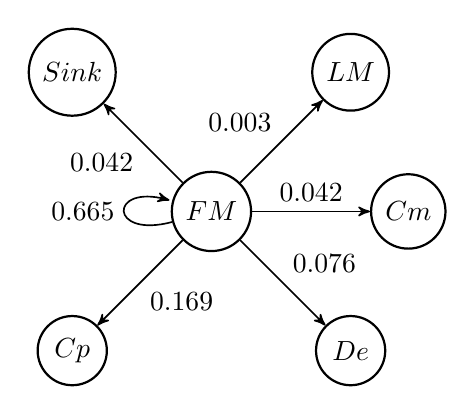
\begin{tikzpicture}[->, >=stealth', auto, semithick, node distance=2.5cm]
\tikzstyle{every state}=[fill=white,draw=black,thick,text=black,scale=1]
\node[state]    (A)                     {$FM$};
%\node[state]    (B)[above right of=A]   {$AS$};
%\node[state]    (C)[above left of=B]    {$Bl$};
%\node[state]    (D)[left of=C]          {$CS$};
%\node[state]    (E)[below right of=A]   {$CC$};
%\node[state]    (F)[below left of=E]    {$LC$};
%\node[state]    (G)[below right of=B]   {$LZC$};
%\node[state]    (H)[below right of =G]  {$LM$};
\node[state]    (H)[above right of =A]  {$LM$};
%\node[state]    (R)[below right of =H]  {$LP$};
%\node[state]    (I)[below left of=H]    {$MCh$};
%\node[state]    (J)[above right of=B]   {$RP$};
%\node[state]    (K)[above right of=G]   {$SC$};
%\node[state]    (L)[above of=B]         {$SG$};
%\node[state]    (M)[below right of=K]   {$SA$};
%\node[state]    (N)[above of=D]         {$Bu$};
%\node[state]    (O)[left of=D]          {$Source$};
%\node[state]    (P)[below right of=O]   {$Cm$};
\node[state]    (P)[right of=A]   {$Cm$};
%\node[state]    (Q)[below left of=P]   {$Cp$};
\node[state]    (Q)[below left of=A]   {$Cp$};
%\node[state]    (R)[below left of=A]    {$FM$};
%\node[state]    (S)[above right of=K]   {$Sink$};
\node[state]    (S)[above left of=A]   {$Sink$};
%\node[state]	(V)[below left of=O]	 {$De$};
\node[state]	(V)[below right of=A]	 {$De$};
%\node[state]    (U)[below right of=N]    {$Ob$};
%\node[state]    (Y)[above right of=O]   {$PT$};
%\node[state]    (Z)[above left of=O]   {$Si$};

\path
(A) edge[loop left]     node{$0.665$}   (A)
edge        node{$0.003$}       (H)
edge         node{$0.042$}      (P)
edge       node{$0.169$}        (Q)
edge        node{$0.076$}       (V)
edge         node{$0.042$}      (S);

\end{tikzpicture}
}
\caption{FactoryMethod (FM) mutation in Eclipse.}
\label{Figure:FM-Mutations-Eclipse}
\end{center}
\end{figure*}


\begin{figure}%[ht]
\begin{center}
\scalebox{0.7}{
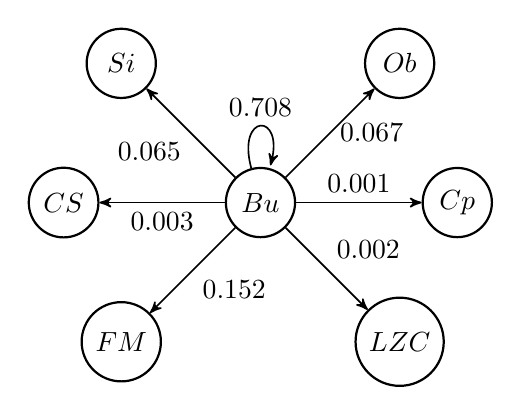
\begin{tikzpicture}[->, >=stealth', auto, semithick, node distance=2.5cm]
\tikzstyle{every state}=[fill=white,draw=black,thick,text=black,scale=1]
\node[state]    (A)                     {$Bu$};
%\node[state]    (B)[above right of=A]   {$AS$};
%\node[state]    (C)[above left of=B]    {$Bl$};
%\node[state]    (D)[left of=C]          {$CS$};
\node[state]    (D)[left of=A]          {$CS$};
%\node[state]    (E)[below right of=A]   {$CC$};
%\node[state]    (F)[below left of=E]    {$LC$};
%\node[state]    (G)[below right of=B]   {$LZC$};
\node[state]    (G)[below right of=A]   {$LZC$};
%\node[state]    (H)[below right of =G]  {$LM$};
%\node[state]    (R)[below right of =H]  {$LP$};
%\node[state]    (I)[below left of=H]    {$MCh$};
%\node[state]    (J)[above right of=B]   {$RP$};
%\node[state]    (K)[above right of=G]   {$SC$};
%\node[state]    (L)[above of=B]         {$SG$};
%\node[state]    (M)[below right of=K]   {$SA$};
%\node[state]    (N)[below left of=D]    {$Bu$};
%\node[state]    (O)[below left of=N]    {$Source$};
%\node[state]    (P)[below right of=O]   {$Cm$};
%\node[state]    (Q)[left of=A]          {$Cp$};
\node[state]    (Q)[right of=A]          {$Cp$};
%\node[state]    (R)[below left of=A]    {$FM$};
\node[state]    (R)[below left of=A]    {$FM$};
%\node[state]    (S)[above right of=K]   {$Sink$};
%\node[state]	(V)[right of=O]	        {$De$};
%\node[state]    (U)[below right of=N]   {$Ob$};
\node[state]    (U)[above right of=A]   {$Ob$};
%\node[state]    (Y)[above right of=O]   {$PT$};
\node[state]    (Z)[above left of=A]    {$Si$};

\path
(A) edge[loop above]     node{$0.708$}   (A)
edge        node{$0.003$}       (D)
edge         node{$0.002$}      (G)
edge       node{$0.001$}        (Q)
edge        node{$0.152$}       (R)
edge [right]        node{$0.067$}      (U)
edge        node{$0.065$}       (Z);

\end{tikzpicture}
}
\caption{Builder (Bu) mutation in Nuxeo.}
\label{Figure:Bu-Mutations-Nuxeo}
\end{center}
\end{figure} 

\begin{figure}
\begin{center}
\scalebox{0.7}{
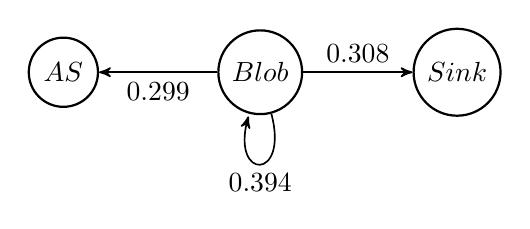
\begin{tikzpicture}[->, >=stealth', auto, semithick, node distance=2.5cm]
\tikzstyle{every state}=[fill=white,draw=black,thick,text=black,scale=1]
\node[state]    (A)                     {$Blob$};
\node[state]    (B)[left of=A]   {$AS$};
%\node[state]    (C)[above left of=B]    {$LP$};
%\node[state]    (D)[left of=C]          {$CS$};
%\node[state]    (E)[below right of=A]   {$CC$};
%\node[state]    (F)[below left of=E]    {$LC$};
%\node[state]    (G)[below right of=B]   {$LZC$};
%\node[state]    (H)[below right of =G]  {$LM$};
%\node[state]    (I)[below left of=H]    {$MCh$};
%\node[state]    (J)[above right of=B]   {$RP$};
%\node[state]    (K)[above right of=G]   {$SC$};
%\node[state]    (L)[above of=B]         {$SG$};
%\node[state]    (M)[below right of=K]   {$SA$};
%\node[state]    (N)[above of=D]         {$Bu$};
%\node[state]    (O)[left of=D]          {$Source$};
%\node[state]    (P)[below right of=O]   {$Cm$};
%\node[state]    (Q)[below left of=P]    {$Cp$};
%\node[state]    (R)[below left of=A]    {$FM$};
%\node[state]    (S)[above right of=K]   {$Sink$};
\node[state]    (S)[right of=A]   {$Sink$};
%\node[state]	(V)[below left of=R]	{$De$};
%\node[state]    (U)[below right of=N]    {$Ob$};
%\node[state]    (Y)[above right of=O]   {$PT$};
%\node[state]    (Z)[below left of=O]    {$Si$};

\path
(A) edge[loop below]     node{$0.394$}   (A)
edge        node{$0.299$}       (B)
edge         node{$0.308$}      (S);

\end{tikzpicture}
}
\caption{Blob (Bl) mutation in oVirt.}
\label{Figure:Bl-Mutations-Ovirt}
\end{center}
\end{figure}



\begin{figure*}
\begin{center}
\scalebox{0.8}{
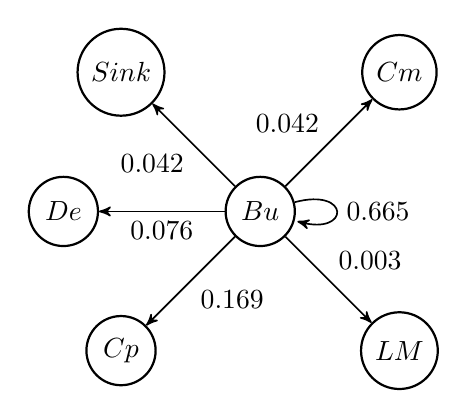
\begin{tikzpicture}[->, >=stealth', auto, semithick, node distance=2.5cm]
\tikzstyle{every state}=[fill=white,draw=black,thick,text=black,scale=1]
\node[state]    (A)                     {$Bu$};
%\node[state]    (B)[above right of=A]   {$AS$};
%\node[state]    (C)[above left of=B]    {$Bl$};
%\node[state]    (D)[left of=C]          {$CS$};
%\node[state]    (E)[below right of=A]   {$CC$};
%\node[state]    (F)[below left of=E]    {$LC$};
%\node[state]    (G)[below right of=B]   {$LZC$};
%\node[state]    (H)[below right of =G]  {$LM$};
\node[state]    (H)[below right of =A]  {$LM$};
%\node[state]    (R)[below right of =H]  {$LP$};
%\node[state]    (I)[below left of=H]    {$MCh$};
%\node[state]    (J)[above right of=B]   {$RP$};
%\node[state]    (K)[above right of=G]   {$SC$};
%\node[state]    (L)[above of=B]         {$SG$};
%\node[state]    (M)[below right of=K]   {$SA$};
%\node[state]    (N)[below left of=D]    {$Bu$};
%\node[state]    (O)[below left of=N]    {$Source$};
%\node[state]    (P)[below right of=O]   {$Cm$};
\node[state]    (P)[above right of=A]   {$Cm$};
%\node[state]    (Q)[below left of=P]   {$Cp$};
\node[state]    (Q)[below left of=A]   {$Cp$};
%\node[state]    (R)[below left of=A]    {$FM$};
%\node[state]    (S)[above right of=K]   {$Sink$};
\node[state]    (S)[above left of=A]   {$Sink$};
%\node[state]	(V)[right of=O]	        {$De$};
\node[state]	(V)[left of=A]	        {$De$};
%\node[state]    (U)[below right of=N]   {$Ob$};
%\node[state]    (Y)[above right of=O]   {$PT$};
%\node[state]    (Z)[above left of=O]    {$Si$};


\path
(A) edge[loop right]     node{$0.665$}   (A)
edge        node{$0.003$}       (H)
edge         node{$0.042$}      (P)
edge       node{$0.169$}        (Q)
edge        node{$0.076$}       (V)
edge         node{$0.042$}      (S);

\end{tikzpicture}
}
\caption{Builder (Bu) mutation among the different snapshots of Matsim.}
\label{Figure:Bu-Mutations-Matsim}
\end{center}
\end{figure*}

\begin{landscape}
\begin{table*}
\caption{Change probabilities of design anti-patterns and design patterns in oVirt}
\setlength\tabcolsep{0.08cm}% let LaTeX calculate intercolumn whitespace
\scriptsize
\centering
\scalebox{0.73}{
{\renewcommand{\arraystretch}{1.05}
\begin{tabular}
{|l|l||l|l|l|l|l|l|l|l|l|l|l|l|l||l|l|l|l|l|l|l|l||p{0.7cm}|p{0.9cm}}
\cline{2-24}
\multicolumn{1}{l|}{}& Source & AS & Bl & CS & CC & LC & LZC & LM & LP & MCh & RP & SC & SG & SA & Bu & Cm & Cp & FM & De & Ob & PT & Si & Sink \\
\hline
AS & 0.018 & \cellcolor[gray]{0.8}{\textbf{0.971}} & 0.000 & 0.000 & 0.000 & 0.000 & 0.000 & 0.000 & 0.000 & 0.000 & 0.000 & 0.000 & 0.000 & 0.000 & 0.000 & 0.000 & 0.000 & 0.000 & 0.000 & 0.000 & 0.000 & 0.000 & 0.011\\
\hline
Bl & 0.000 & \cellcolor[gray]{0.8}{\textbf{0.299}} & \cellcolor[gray]{0.8}{\textbf{0.394}} & 0.000 & 0.000 & 0.000 & 0.000 & 0.000 & 0.000 & 0.000 & 0.000 & 0.000 & 0.000 & 0.000 & 0.000 & 0.000 & 0.000 & 0.000 & 0.000 & 0.000 & 0.000 & 0.000 & \cellcolor[gray]{0.8}{\textbf{0.308}}\\
\hline
CS & 0.006 & 0.000 & 0.003 & \cellcolor[gray]{0.8}{\textbf{0.982}} & 0.000 & 0.000 & 0.000 & 0.000 & 0.000 & 0.000 & 0.000 & 0.000 & 0.000 & 0.000 & 0.000 & 0.000 & 0.000 & 0.000 & 0.000 & 0.000 & 0.000 & 0.000 & 0.009 \\
\hline
CC & 0.000 & 0.000 & 0.000 & 0.012 & \cellcolor[gray]{0.8}{\textbf{0.975}} & 0.000 & 0.000 & 0.000 & 0.000 & 0.000 & 0.000 & 0.000 & 0.000 & 0.000 & 0.000 & 0.000 & 0.000 & 0.000 & 0.000 & 0.000 & 0.000 & 0.000 & 0.013 \\
\hline
LC & 0.000 & 0.000 & 0.000 & 0.000 & 0.000 & \cellcolor[gray]{0.8}{\textbf{1}} & 0.000 & 0.000 & 0.000 & 0.000 & 0.000 & 0.000 & 0.000 & 0.000 & 0.000 & 0.000 & 0.000 & 0.000 & 0.000 & 0.000 & 0.000 & 0.000 & 0.000 \\
\hline
LZC & 0.000 & 0.000 & 0.000 & 0.000 & 0.000 & 0.001 & \cellcolor[gray]{0.8}{\textbf{0.998}} & 0.000 & 0.000 & 0.000 & 0.000 & 0.000 & 0.000 & 0.000 & 0.000 & 0.000 & 0.000 & 0.000 & 0.000 & 0.000 & 0.000 & 0.000 & 0.001 \\
\hline
LM & 0.000 & 0.000 & 0.000 & 0.000 & 0.000 & 0.000 & 0.012 & \cellcolor[gray]{0.8}{\textbf{0.977}} & 0.000 & 0.000 & 0.000 & 0.000 & 0.000 & 0.000 & 0.000 & 0.000 & 0.000 & 0.000 & 0.000 & 0.000 & 0.000 & 0.000 & 0.011 \\
\hline
LP & 0.000 & 0.000 & 0.000 & 0.000 & 0.000 & 0.000 & 0.000 & 0.008 & \cellcolor[gray]{0.8}{\textbf{0.969}} & 0.000 & 0.000 & 0.000 & 0.000 & 0.000 & 0.000 & 0.000 & 0.000 & 0.000 & 0.000 & 0.000 & 0.000 & 0.000 & 0.022 \\
\hline
MCh & 0.000 & 0.000 & 0.000 & 0.000 & 0.000 & 0.000 & 0.000 & 0.000 & 0.000 & \cellcolor[gray]{0.8}{\textbf{1}} & 0.000 & 0.000 & 0.000 & 0.000 & 0.000 & 0.000 & 0.000 & 0.000 & 0.000 & 0.000 & 0.000 & 0.000 & 0.000 \\
\hline
RP & 0.000 & 0.000 & 0.000 & 0.000 & 0.000 & 0.000 & 0.000 & 0.000 & 0.000 & 0.082 & \cellcolor[gray]{0.8}{\textbf{0.857}} & 0.000 & 0.000 & 0.000 & 0.000 & 0.000 & 0.000 & 0.000 & 0.000 & 0.000 & 0.000 & 0.000 & 0.061 \\
\hline
SC & 0.000 & 0.000 & 0.000 & 0.000 & 0.000 & 0.000 & 0.000 & 0.000 & 0.000 & 0.000 & 0.000 & \cellcolor[gray]{0.8}{\textbf{1}} & 0.000 & 0.000 & 0.000 & 0.000 & 0.000 & 0.000 & 0.000 & 0.000 & 0.000 & 0.000 & 0.000 \\
\hline 
SG & 0.000 & 0.000 & 0.000 & 0.000 & 0.000 & 0.000 & 0.000 & 0.000 & 0.000 & 0.000 & 0.000 & 0.000 & \cellcolor[gray]{0.8}{\textbf{1}} & 0.000 & 0.000 & 0.000 & 0.000 & 0.000 & 0.000 & 0.000 & 0.000 & 0.000 & 0.000\\
\hline
SA & 0.000 & 0.000 & 0.000 & 0.000 & 0.000 & 0.000 & 0.000 & 0.000 & 0.000 & 0.000 & 0.000 & 0.000 & 0.000 & \cellcolor[gray]{0.8}{\textbf{1}} & 0.000 & 0.000 & 0.000 & 0.000 & 0.000 & 0.000 & 0.000 & 0.000 & 0.000 \\
\hline \hline
Bu & 0.000 & 0.000 & 0.000 & 0.000 & 0.000 & 0.000 & 0.000 & 0.000 & 0.000 & 0.000 & 0.000 & 0.000 & 0.000 & 0.000 & \cellcolor[gray]{0.8}{\textbf{1}} & 0.000 & 0.000 & 0.000 & 0.000 & 0.000 & 0.000 & 0.000 & 0.000 \\
\hline 
Cm & 0.000 & 0.000 & 0.000 & 0.000 & 0.000 & 0.000 & 0.000 & 0.000 & 0.000 & 0.000 & 0.000 & 0.000 & 0.000 & 0.019 & 0.000 & \cellcolor[gray]{0.8}{\textbf{1}} & 0.000 & 0.000 & 0.000 & 0.000 & 0.000 & 0.000 & 0.000 \\
\hline
Cp & 0.000 & 0.000 & 0.000 & 0.000 & 0.000 & 0.000 & 0.000 & 0.000 & 0.000 & 0.000 & 0.000 & 0.000 & 0.000 & 0.000 & 0.000 & 0.000 & \cellcolor[gray]{0.8}{\textbf{1}} & 0.000 & 0.000 & 0.000 & 0.000 & 0.000 & 0.000 \\
\hline
FM & 0.000 & 0.000 & 0.000 & 0.000 & 0.000 & 0.000 & 0.000 & 0.000 & 0.000 & 0.000 & 0.000 & 0.000 & 0.000 & 0.000 & 0.000 & 0.000 & 0.000 & \cellcolor[gray]{0.8}{\textbf{1}} & 0.000 & 0.000 & 0.000 & 0.000 & 0.000 \\
\hline
De & 0.000 & 0.000 & 0.000 & 0.000 & 0.000 & 0.000 & 0.000 & 0.000 & 0.000 & 0.000 & 0.000 & 0.000 & 0.000 & 0.000 & 0.000 & 0.000 & 0.000 & 0.000 & \cellcolor[gray]{0.8}{\textbf{1}} & 0.000 & 0.000 & 0.000 & 0.000 \\
\hline
Ob & 0.000 & 0.000 & 0.000 & 0.000 & 0.000 & 0.000 & 0.000 & 0.000 & 0.000 & 0.000 & 0.000 & 0.000 & 0.000 & 0.000 & 0.000 & 0.000 & 0.000 & 0.000 & 0.000 & \cellcolor[gray]{0.8}{\textbf{1}} & 0.000 & 0.000 & 0.000 \\
\hline
PT & 0.000 & 0.000 & 0.000 & 0.000 & 0.000 & 0.000 & 0.000 & 0.000 & 0.000 & 0.000 & 0.000 & 0.000 & 0.000 & 0.000 & 0.000 & 0.000 & 0.000 & 0.000 & 0.000 & 0.000 & \cellcolor[gray]{0.8}{\textbf{1}} & 0.000 & 0.000 \\
\hline
Si & 0.000 & 0.001 & 0.000 & 0.000 & 0.000 & 0.000 & 0.000 & 0.000 & 0.000 & 0.000 & 0.000 & 0.000 & 0.000 & 0.000 & 0.000 & 0.000 & 0.000 & 0.000 & 0.000 & 0.000 & \cellcolor[gray]{0.8}{\textbf{0.097}} & \cellcolor[gray]{0.8}{\textbf{0.798}} & \cellcolor[gray]{0.8}{\textbf{0.103}} \\
\hline
\end{tabular}
}}
\label{tab:Ovirtmarkov}
\end{table*}

\begin{table*} %[ht] 
\caption{Change probabilities of design anti-patterns and design patterns in Matsim}
\setlength\tabcolsep{0.08cm}% let LaTeX calculate intercolumn whitespace
\scriptsize
\centering
\scalebox{0.73}{
{\renewcommand{\arraystretch}{1.05}
\begin{tabular}
{|l|l||l|l|l|l|l|l|l|l|l|l|l|l|l||l|l|l|l|l|l|l|l||p{0.7cm}|p{0.9cm}}
\cline{2-24}
\multicolumn{1}{l|}{}& Source & AS & Bl & CS & CC & LC & LZC & LM & LP & MCh & RP & SC & SG & SA & Bu & Cm & Cp & FM & De & Ob & PT & Si & Sink \\
\hline
AS & 0.066 & \cellcolor[gray]{0.8}{\textbf{0.893}} & 0.000 & 0.000 & 0.000 & 0.000 & 0.000 & 0.000 & 0.000 & 0.000 & 0.000 & 0.000 & 0.000 & 0.000 & 0.000 & 0.000 & 0.000 & 0.040 & 0.000 & 0.000 & 0.000 & 0.000 & 0.000\\
\hline
Bl & 0.003 & \cellcolor[gray]{0.8}{\textbf{0.372}} & \cellcolor[gray]{0.8}{\textbf{0.279}} & 0.000 & 0.000 & 0.000 & 0.000 & 0.000 & 0.000 & 0.000 & 0.000 & 0.000 & 0.000 & 0.000 & 0.000 & 0.000 & 0.000 & \cellcolor[gray]{0.8}{\textbf{0.346}} & 0.000 & 0.000 & 0.000 & 0.000 & 0.000\\
\hline
CS & 0.025 & 0.000 & 0.037 & \cellcolor[gray]{0.8}{\textbf{0.9}} & 0.000 & 0.000 & 0.000 & 0.000 & 0.000 & 0.000 & 0.000 & 0.000 & 0.000 & 0.000 & 0.000 & 0.000 & 0.000 & 0.038 & 0.000 & 0.000 & 0.000 & 0.000 & 0.000 \\
\hline
CC & 0.004 & 0.001 & 0.002 & 0.075 & \cellcolor[gray]{0.8}{\textbf{0.848}} & 0.000 & 0.000 & 0.000 & 0.000 & 0.000 & 0.000 & 0.000 & 0.000 & 0.000 & 0.000 & 0.000 & 0.000 & 0.069 & 0.000 & 0.000 & 0.000 & 0.000 & 0.000 \\
\hline
LC & 0.000 & 0.000 & 0.000 & 0.000 & 0.000 & \cellcolor[gray]{0.8}{\textbf{1}} & 0.000 & 0.000 & 0.000 & 0.000 & 0.000 & 0.000 & 0.000 & 0.000 & 0.000 & 0.000 & 0.000 & 0.000 & 0.000 & 0.000 & 0.000 & 0.000 & 0.000 \\
\hline
LZC & 0.000 & 0.003 & 0.000 & 0.000 & 0.000 & \cellcolor[gray]{0.8}{\textbf{0.1}} & \cellcolor[gray]{0.8}{\textbf{0.831}} & 0.000 & 0.000 & 0.000 & 0.000 & 0.000 & 0.000 & 0.000 & 0.000 & 0.000 & 0.000 & 0.066 & 0.000 & 0.000 & 0.000 & 0.000 & 0.000 \\
\hline
LM & 0.003 & 0.001 & 0.002 & 0.013 & 0.000 & 0.000 & 0.063 & \cellcolor[gray]{0.8}{\textbf{0.86}} & 0.000 & 0.000 & 0.000 & 0.000 & 0.000 & 0.000 & 0.000 & 0.000 & 0.000 & 0.059 & 0.000 & 0.000 & 0.000 & 0.000 & 0.000 \\
\hline
LP & 0.003 & 0.000 & 0.003 & 0.013 & 0.000 & 0.000 & 0.007 & 0.034 & \cellcolor[gray]{0.8}{\textbf{0.887}} & 0.000 & 0.000 & 0.000 & 0.000 & 0.000 & 0.000 & 0.000 & 0.000 & 0.053 & 0.000 & 0.000 & 0.000 & 0.000 & 0.000 \\
\hline
MCh & 0.000 & 0.000 & 0.000 & 0.000 & 0.000 & 0.000 & 0.000 & 0.000 & 0.000 & \cellcolor[gray]{0.8}{\textbf{1}} & 0.000 & 0.000 & 0.000 & 0.000 & 0.000 & 0.000 & 0.000 & 0.000 & 0.000 & 0.000 & 0.000 & 0.000 & 0.000 \\
\hline
RP & 0.000 & 0.000 & 0.000 & 0.000 & 0.000 & 0.000 & 0.000 & 0.000 & 0.000 & 0.021 & \cellcolor[gray]{0.8}{\textbf{0.596}} & 0.000 & 0.000 & 0.000 & 0.000 & 0.000 & 0.000 & \cellcolor[gray]{0.8}{\textbf{0.193}} & 0.000 & 0.000 & 0.000 & 0.000 & 0.000 \\
\hline
SC & 0.026 & 0.000 & 0.000 & 0.000 & 0.000 & 0.000 & 0.003 & 0.000 & 0.000 & 0.000 & 0.038 & \cellcolor[gray]{0.8}{\textbf{0.834}} & 0.000 & 0.000 & 0.000 & 0.000 & 0.000 & \cellcolor[gray]{0.8}{\textbf{0.099}} & 0.000 & 0.000 & 0.000 & 0.000 & 0.000 \\
\hline 
SG & 0.000 & 0.000 & 0.000 & 0.091 & 0.000 & 0.000 & 0.000 & 0.000 & 0.000 & 0.000 & 0.000 & \cellcolor[gray]{0.8}{\textbf{0.182}} & \cellcolor[gray]{0.8}{\textbf{0.455}} & 0.000 & 0.000 & 0.000 & 0.000 & \cellcolor[gray]{0.8}{\textbf{0.273}} & 0.000 & 0.000 & 0.000 & 0.000 & 0.000\\
\hline
SA & 0.000 & 0.000 & 0.000 & 0.000 & 0.000 & 0.000 & 0.000 & 0.000 & 0.000 & 0.000 & 0.000 & 0.000 & 0.000 & \cellcolor[gray]{0.8}{\textbf{1}} & 0.000 & 0.000 & 0.000 & 0.000 & 0.000 & 0.000 & 0.000 & 0.000 & 0.000 \\
\hline \hline
Bu & 0.000 & 0.000 & 0.000 & 0.001 & 0.000 & 0.000 & 0.003 & 0.000 & 0.000 & 0.000 & 0.000 & 0.000 & 0.000 & 0.000 & \cellcolor[gray]{0.8}{\textbf{0.546}} & 0.000 & 0.001 & \cellcolor[gray]{0.8}{\textbf{0.272}} & 0.000 & \cellcolor[gray]{0.8}{\textbf{0.141}} & 0.000 & 0.030 & 0.000 \\
\hline
Cm & 0.000 & 0.000 & 0.000 & 0.001 & 0.000 & 0.000 & 0.002 & 0.000 & 0.000 & 0.000 & 0.000 & 0.000 & 0.000 & 0.030 & 0.000 & \cellcolor[gray]{0.8}{\textbf{0.371}} & 0.075 & \cellcolor[gray]{0.8}{\textbf{0.387}} & \cellcolor[gray]{0.8}{\textbf{0.117}} & 0.012 & 0.000 & 0.000 & 0.000 \\
\hline
Cp & 0.000 & 0.000 & 0.000 & 0.002 & 0.000 & 0.000 & 0.003 & 0.000 & 0.000 & 0.000 & 0.000 & 0.000 & 0.000 & 0.000 & 0.037 & 0.044 & \cellcolor[gray]{0.8}{\textbf{0.850}} & 0.061 & 0.000 & 0.000 & 0.000 & 0.000 & 0.000 \\
\hline
FM & 0.000 & 0.000 & 0.000 & 0.001 & 0.000 & 0.000 & 0.001 & 0.001 & 0.000 & 0.000 & 0.000 & 0.000 & 0.000 & 0.000 & 0.000 & 0.036 & 0.074 & \cellcolor[gray]{0.8}{\textbf{0.825}} & 0.059 & 0.000 & 0.000 & 0.000 & 0.000 \\
\hline
De & 0.000 & 0.000 & 0.000 & 0.000 & 0.000 & 0.000 & 0.000 & 0.000 & 0.000 & 0.000 & 0.000 & 0.000 & 0.000 & 0.000 & 0.000 & 0.000 & 0.000 & 0.049 & \cellcolor[gray]{0.8}{\textbf{0.912}} & 0.034 & 0.000 & 0.000 & 0.000 \\
\hline
Ob & 0.000 & 0.000 & 0.000 & 0.000 & 0.000 & 0.000 & 0.000 & 0.000 & 0.000 & 0.000 & 0.000 & 0.000 & 0.000 & 0.000 & 0.000 & 0.000 & 0.000 & 0.000 & 0.000 & \cellcolor[gray]{0.8}{\textbf{1}} & 0.000 & 0.000 & 0.000 \\
\hline
PT & 0.000 & 0.000 & 0.000 & 0.000 & 0.000 & 0.000 & 0.000 & 0.000 & 0.000 & 0.000 & 0.000 & 0.000 & 0.000 & 0.000 & 0.000 & 0.000 & 0.000 & 0.000 & 0.000 & 0.000 & \cellcolor[gray]{0.8}{\textbf{1}} & 0.000 & 0.000 \\
\hline
Si & 0.000 & 0.000 & 0.000 & 0.000 & 0.000 & 0.000 & 0.001 & 0.000 & 0.000 & 0.000 & 0.000 & 0.000 & 0.000 & 0.000 & 0.000 & 0.000 & 0.000 & 0.028 & 0.000 & 0.000 & 0.009 & \cellcolor[gray]{0.8}{\textbf{0.962}} & 0.000 \\
\hline
\end{tabular}
}}
\label{tab:MatsimMarkov}
\end{table*}
\end{landscape}



% \begin{landscape}

% \end{landscape}


\begin{landscape}
\begin{table*}%[ht] 
\caption{Change probabilities of design anti-patterns and design patterns in ApacheSolr}
\setlength\tabcolsep{0.08cm}% let LaTeX calculate intercolumn whitespace
\scriptsize
\centering
\scalebox{0.73}{
{\renewcommand{\arraystretch}{1.05}
\begin{tabular}
{|l|l||l|l|l|l|l|l|l|l|l|l|l|l|l||l|l|l|l|l|l|l|l||p{0.9cm}|p{0.9cm}}
\cline{2-24}
\multicolumn{1}{l|}{}& Source & AS & Bl & CS & CC & LC & LZC & LM & LP & MCh & RP & SC & SG & SA & Bu & Cm & Cp & FM & De & Ob & PT & Si & Sink \\
\hline
AS & 0.000 & \cellcolor[gray]{0.8}{\textbf{1}} & 0.000 & 0.000 & 0.000 & 0.000 & 0.000 & 0.000 & 0.000 & 0.000 & 0.000 & 0.000 & 0.000 & 0.000 & 0.000 & 0.000 & 0.000 & 0.000 & 0.000 & 0.000 & 0.000 & 0.000 & 0.000 \\
\hline
Bl & 0.000 & \cellcolor[gray]{0.8}{\textbf{0.321}} & \cellcolor[gray]{0.8}{\textbf{0.365}} & 0.000 & 0.000 & 0.000 & 0.000 & 0.000 & 0.000 & 0.000 & 0.000 & 0.000 & 0.000 & 0.000 & 0.000 & 0.000 & 0.000 & 0.000 & 0.000 & 0.000 & 0.000 & 0.000 & \cellcolor[gray]{0.8}{\textbf{0.313}} \\
\hline
CS & 0.000 & 0.000 & 0.009 & \cellcolor[gray]{0.8}{\textbf{0.983}} & 0.000 & 0.000 & 0.000 & 0.000 & 0.000 & 0.000 & 0.000 & 0.000 & 0.000 & 0.000 & 0.000 & 0.000 & 0.000 & 0.000 & 0.000 & 0.000 & 0.000 & 0.000 & 0.008 \\
\hline
CC & 0.000 & 0.000 & 0.000 & 0.033 & \cellcolor[gray]{0.8}{\textbf{0.93}} & 0.000 & 0.000 & 0.000 & 0.000 & 0.000 & 0.000 & 0.000 & 0.000 & 0.000 & 0.000 & 0.000 & 0.000 & 0.000 & 0.000 & 0.000 & 0.000 & 0.000 & 0.037 \\
\hline
LC & 0.000 & 0.000 & 0.000 & 0.000 & 0.000 & \cellcolor[gray]{0.8}{\textbf{1}} & 0.000 & 0.000 & 0.000 & 0.000 & 0.000 & 0.000 & 0.000 & 0.000 & 0.000 & 0.000 & 0.000 & 0.000 & 0.000 & 0.000 & 0.000 & 0.000 & 0.000 \\
\hline
LZC & 0.000 & 0.000 & 0.000 & 0.000 & 0.000 & 0.072 & \cellcolor[gray]{0.8}{\textbf{0.859}} & 0.000 & 0.000 & 0.000 & 0.000 & 0.000 & 0.000 & 0.000 & 0.000 & 0.000 & 0.000 & 0.000 & 0.000 & 0.000 & 0.000 & 0.000 & 0.069 \\
\hline
LM & 0.000 & 0.000 & 0.001 & 0.002 & 0.000 & 0.000 & 0.033 & \cellcolor[gray]{0.8}{\textbf{0.928}} & 0.000 & 0.000 & 0.000 & 0.000 & 0.000 & 0.000 & 0.000 & 0.000 & 0.000 & 0.000 & 0.000 & 0.000 & 0.000 & 0.000 & 0.036 \\
\hline
LP & 0.000 & 0.001 & 0.000 & 0.008 & 0.000 & 0.000 & 0.007 & 0.079 & \cellcolor[gray]{0.8}{\textbf{0.779}} & 0.000 & 0.000 & 0.000 & 0.000 & 0.000 & 0.000 & 0.000 & 0.000 & 0.000 & 0.000 & 0.000 & 0.000 & 0.000 & 0.125 \\
\hline
MCh & 0.000 & 0.000 & 0.000 & 0.000 & 0.000 & 0.000 & 0.000 & 0.000 & 0.000 & \cellcolor[gray]{0.8}{\textbf{1}} & 0.000 & 0.000 & 0.000 & 0.000 & 0.000 & 0.000 & 0.000 & 0.000 & 0.000 & 0.000 & 0.000 & 0.000 & 0.000 \\
\hline
RP & 0.000 & 0.000 & 0.000 & 0.000 & 0.000 & 0.000 & 0.000 & 0.000 & 0.000 & 0.088 & \cellcolor[gray]{0.8}{\textbf{0.84}} & 0.000 & 0.000 & 0.000 & 0.000 & 0.000 & 0.000 & 0.000 & 0.000 & 0.000 & 0.000 & 0.000 & 0.072 \\
\hline
SC & 0.000 & 0.000 & 0.000 & 0.000 & 0.000 & 0.000 & 0.000 & 0.000 & 0.000 & 0.000 & 0.000 & \cellcolor[gray]{0.8}{\textbf{1}} & 0.000 & 0.000 & 0.000 & 0.000 & 0.000 & 0.000 & 0.000 & 0.000 & 0.000 & 0.000 & 0.000\\
\hline
SG & 0.000 & 0.000 & 0.000 & 0.000 & 0.000 & 0.000 & 0.000 & 0.000 & 0.000 & 0.000 & 0.013 & 0.000 &  \cellcolor[gray]{0.8}{\textbf{0.981}} & 0.000 & 0.000 & 0.000 & 0.000 & 0.000 & 0.000 & 0.000 & 0.000 & 0.000 & 0.006 \\
\hline
SA & 0.000 & 0.000 & 0.000 & 0.000 & 0.000 & 0.000 & 0.000 & 0.000 & 0.000 & 0.000 & 0.000 & 0.000 & 0.000 & \cellcolor[gray]{0.8}{\textbf{1}} & 0.000 & 0.000 & 0.000 & 0.000 & 0.000 & 0.000 & 0.000 & 0.000 & 0.000 \\
\hline \hline
Bu & 0.000 & 0.000 & 0.000 & 0.000 & 0.000 & 0.000 & 0.000 & 0.000 & 0.000 & 0.000 & 0.000 & 0.000 & 0.000 & 0.000 & \cellcolor[gray]{0.8}{\textbf{0.963}} & 0.000 & 0.000 & 0.000 & 0.000 & 0.005 & 0.000 & 0.000 & 0.027 \\
\hline
Cm & 0.000 & 0.000 & 0.000 & 0.000 & 0.000 & 0.000 & 0.000 & 0.000 & 0.000 & 0.000 & 0.000 & 0.000 & 0.000 & 0.000 & 0.000 & \cellcolor[gray]{0.8}{\textbf{1}} & 0.000 & 0.000 & 0.000 & 0.000 & 0.000 & 0.000 & 0.000 \\
\hline
Cp & 0.000 & 0.000 & 0.000 & 0.000 & 0.000 & 0.000 & 0.000 & 0.000 & 0.000 & 0.000 & 0.000 & 0.000 & 0.000 & 0.000 & 0.000 & 0.000 & \cellcolor[gray]{0.8}{\textbf{1}} & 0.000 & 0.000 & 0.000 & 0.000 & 0.000 & 0.000 \\
\hline
FM & 0.000 & 0.000 & 0.000 & 0.000 & 0.000 & 0.000 & 0.000 & 0.000 & 0.000 & 0.000 & 0.000 & 0.000 & 0.000 & 0.000 & 0.000 & 0.000 & 0.012 & \cellcolor[gray]{0.8}{\textbf{0.874}} & 0.005 & 0.000 & 0.000 & 0.000 & 0.092 \\
\hline
De & 0.000 & 0.000 & 0.000 & 0.000 & 0.000 & 0.000 & 0.000 & 0.000 & 0.000 & 0.000 & 0.000 & 0.000 & 0.000 & 0.000 & 0.000 & 0.000 & 0.000 & 0.000 & \cellcolor[gray]{0.8}{\textbf{0.996}} & 0.000 & 0.000 & 0.000 & 0.004 \\
\hline
Ob & 0.000 & 0.000 & 0.000 & 0.000 & 0.000 & 0.000 & 0.000 & 0.000 & 0.000 & 0.000 & 0.000 & 0.000 & 0.000 & 0.000 & 0.000 & 0.000 & 0.000 & 0.000 & 0.000 & \cellcolor[gray]{0.8}{\textbf{1}} & 0.000 & 0.000 & 0.000 \\
\hline
PT & 0.000 & 0.000 & 0.000 & 0.000 & 0.000 & 0.000 & 0.000 & 0.000 & 0.000 & 0.000 & 0.000 & 0.000 & 0.000 & 0.000 & 0.000 & 0.000 & 0.000 & 0.000 & 0.000 & 0.000 & \cellcolor[gray]{0.8}{\textbf{1}} & 0.000 & 0.000 \\
\hline
Si & 0.000 & 0.000 & 0.000 & 0.000 & 0.000 & 0.000 & 0.000 & 0.000 & 0.000 & 0.000 & 0.000 & 0.000 & 0.000 & 0.000 & 0.000 & 0.000 & 0.000 & 0.000 & 0.000 & 0.000 & 0.007 & \cellcolor[gray]{0.8}{\textbf{0.981}} & 0.012 \\
\hline
\end{tabular}
}
}
\label{tab:SolrMarkov}
\end{table*}

\begin{table*} %[ht]
\caption{Change probabilities of design anti-patterns and design patterns in ApacheIgnite}
\setlength\tabcolsep{0.08cm}% let LaTeX calculate intercolumn whitespace
\scriptsize
\centering
\scalebox{0.735}{
{\renewcommand{\arraystretch}{1.05}
\begin{tabular}
{|l|l||l|l|l|l|l|l|l|l|l|l|l|l|l||l|l|l|l|l|l|l|l||p{0.9cm}|p{0.9cm}}
\cline{2-24}
\multicolumn{1}{l|}{}& Source & AS & Bl & CS & CC & LC & LZC & LM & LP & MCh & RP & SC & SG & SA & Bu & Cm & Cp & FM & De & Ob & PT & Si & Sink \\
\hline
AS & 0.000 & \cellcolor[gray]{0.8}{\textbf{1}} & 0.000 & 0.000 & 0.000 & 0.000 & 0.000 & 0.000 & 0.000 & 0.000 & 0.000 & 0.000 & 0.000 & 0.000 & 0.000 & 0.000 & 0.000 & 0.000 & 0.000 & 0.000 & 0.000 & 0.000 & 0.000 \\
\hline
Bl & 0.000 & \cellcolor[gray]{0.8}{\textbf{0.375}} & \cellcolor[gray]{0.8}{\textbf{0.33}} & 0.000 & 0.000 & 0.000 & 0.000 & 0.000 & 0.000 & 0.000 & 0.000 & 0.000 & 0.000 & 0.000 & 0.000 & 0.000 & 0.000 & 0.000 & 0.000 & 0.000 & 0.000 & 0.000 & \cellcolor[gray]{0.8}{\textbf{0.295}} \\
\hline
CS & 0.000 & 0.000 & 0.000 & \cellcolor[gray]{0.8}{\textbf{1}} & 0.000 & 0.000 & 0.000 & 0.000 & 0.000 & 0.000 & 0.000 & 0.000 &  0.000 & 0.000 & 0.000 & 0.000 & 0.000 & 0.000 & 0.000 & 0.000 & 0.000 & 0.000 & 0.000 \\
\hline
CC & 0.000 & 0.000 & 0.000 & 0.053 & \cellcolor[gray]{0.8}{\textbf{0.905}} & 0.000 & 0.000 & 0.000 & 0.000 & 0.000 & 0.000 & 0.000 & 0.000 & 0.000 & 0.000 & 0.000 & 0.000 & 0.000 & 0.000 & 0.000 & 0.000 & 0.000 & 0.042 \\
\hline
LC & 0.000 & 0.000 & 0.000 & 0.000 & 0.000 & \cellcolor[gray]{0.8}{\textbf{1}} & 0.000 & 0.000 & 0.000 & 0.000 & 0.000 & 0.000 & 0.000 & 0.000 & 0.000 & 0.000 & 0.000 & 0.000 & 0.000 & 0.000 & 0.000 & 0.000 & 0.000 \\
\hline
LZC & 0.000 & 0.000 & 0.000 & 0.000 & 0.000 & 0.015 & \cellcolor[gray]{0.8}{\textbf{0.97}} & 0.000 & 0.000 & 0.000 & 0.000 & 0.000 & 0.000 & 0.000 & 0.000 & 0.000 & 0.000 & 0.000 & 0.000 & 0.000 & 0.000 & 0.000 & 0.015 \\
\hline
LM & 0.000 & 0.000 & 0.000 & 0.004 & 0.000 & 0.000 & 0.045 & \cellcolor[gray]{0.8}{\textbf{0.905}} & 0.000 & 0.000 & 0.000 & 0.000 & 0.000 & 0.000 & 0.000 & 0.000 & 0.000 & 0.000 & 0.000 & 0.000 & 0.000 & 0.000 & 0.047 \\
\hline
LP & 0.000 & 0.000 & 0.000 & 0.009 & 0.000 & 0.000 & 0.006 & 0.051 & \cellcolor[gray]{0.8}{\textbf{0.851}} & 0.000 & 0.000 & 0.000 & 0.000 & 0.000 & 0.000 & 0.000 & 0.000 & 0.000 & 0.000 & 0.000 & 0.000 & 0.000 & 0.081 \\
\hline
MCh & 0.000 & 0.000 & 0.000 & 0.000 & 0.000 & 0.000 & 0.000 & 0.000 & 0.000 & \cellcolor[gray]{0.8}{\textbf{1}} & 0.000 & 0.000 & 0.000 & 0.000 & 0.000 & 0.000 & 0.000 & 0.000 & 0.000 & 0.000 & 0.000 & 0.000 & 0.000 \\
\hline
RP & 0.000 & 0.000 & 0.000 & 0.000 & 0.000 & 0.000 & 0.000 & 0.000 & 0.000 & 0.000 & \cellcolor[gray]{0.8}{\textbf{1}} & 0.000 & 0.000 & 0.000 & 0.000 & 0.000 & 0.000 & 0.000 & 0.000 & 0.000 & 0.000 & 0.000 & 0.000 \\
\hline
SC & 0.000 & 0.000 & 0.000 & 0.000 & 0.000 & 0.000 & 0.000 & 0.000 & 0.000 & 0.000 & 0.000 & \cellcolor[gray]{0.8}{\textbf{1}} & 0.000 & 0.000 & 0.000 & 0.000 & 0.000 & 0.000 & 0.000 & 0.000 & 0.000 & 0.000 & 0.000 \\
\hline
SG & 0.000 & 0.000 & 0.000 & 0.000 & 0.000 & 0.000 & 0.000 & 0.000 & 0.000 & 0.000 & 0.000 & 0.000 & \cellcolor[gray]{0.8}{\textbf{1}} & 0.000 & 0.000 & 0.000 & 0.000 & 0.000 & 0.000 & 0.000 & 0.000 & 0.000 & 0.000 \\
\hline
SA & 0.000 & 0.000 & 0.000 & 0.000 & 0.000 & 0.000 & 0.000 & 0.000 & 0.000 & 0.000 & 0.000 & 0.000 & 0.000 & \cellcolor[gray]{0.8}{\textbf{1}} & 0.000 & 0.000 & 0.000 & 0.000 & 0.000 & 0.000 & 0.000 & 0.000 & 0.000 \\
\hline \hline
Bu & 0.000 & 0.000 & 0.000 & 0.000 & 0.000 & 0.000 & 0.000 & 0.000 & 0.000 & 0.000 & 0.000 & 0.000 & 0.000 & 0.000 & \cellcolor[gray]{0.8}{\textbf{0.976}} & 0.000 & 0.000 & 0.000 & 0.000 & 0.004 & 0.000 & 0.000 & 0.018 \\
\hline
Cm & 0.000 & 0.000 & 0.000 & 0.000 & 0.000 & 0.000 & 0.000 & 0.000 & 0.000 & 0.000 & 0.000 & 0.000 & 0.000 & 0.000 & 0.000 & \cellcolor[gray]{0.8}{\textbf{1}} & 0.000 & 0.000 & 0.000 & 0.000 & 0.000 & 0.000 & 0.000 \\
\hline
Cp & 0.000 & 0.000 & 0.000 & 0.000 & 0.000 & 0.000 & 0.000 & 0.000 & 0.000 & 0.000 & 0.000 & 0.000 & 0.000 & 0.000 & 0.000 & 0.000 & \cellcolor[gray]{0.8}{\textbf{1}} & 0.000 & 0.000 & 0.000 & 0.000 & 0.000 & 0.000 \\
\hline
FM & 0.000 & 0.000 & 0.000 & 0.000 & 0.000 & 0.000 & 0.000 & 0.000 & 0.000 & 0.000 & 0.000 & 0.000 & 0.000 & 0.000 & 0.000 & 0.000 & 0.000 & \cellcolor[gray]{0.8}{\textbf{1}} & 0.000 & 0.000 & 0.000 & 0.000 & 0.000 \\
\hline
De & 0.000 & 0.000 & 0.000 & 0.000 & 0.000 & 0.000 & 0.000 & 0.000 & 0.000 & 0.000 & 0.000 & 0.000 & 0.000 & 0.000 & 0.000 & 0.000 & 0.000 & 0.000 & \cellcolor[gray]{0.8}{\textbf{1}} & 0.000 & 0.000 & 0.000 & 0.000 \\
\hline
Ob & 0.000 & 0.000 & 0.000 & 0.000 & 0.000 & 0.000 & 0.000 & 0.000 & 0.000 & 0.000 & 0.000 & 0.000 & 0.000 & 0.000 & 0.000 & 0.000 & 0.000 & 0.000 & 0.000 & \cellcolor[gray]{0.8}{\textbf{1}} & 0.000 & 0.000 & 0.000 \\
\hline
PT & 0.000 & 0.000 & 0.000 & 0.000 & 0.000 & 0.000 & 0.000 & 0.000 & 0.000 & 0.000 & 0.000 & 0.000 & 0.000 & 0.000 & 0.000 & 0.000 & 0.000 & 0.000 & 0.000 & 0.000 & \cellcolor[gray]{0.8}{\textbf{1}} & 0.000 & 0.000 \\
\hline
Si & 0.000 & 0.000 & 0.000 & 0.000 & 0.000 & 0.000 & 0.000 & 0.000 & 0.000 & 0.000 & 0.000 & 0.000 & 0.000 & 0.000 & 0.000 & 0.000 & 0.000 & 0.000 & 0.000 & 0.000 & 0.003 & \cellcolor[gray]{0.8}{\textbf{0.994}} & 0.003 \\
\hline
\end{tabular}
}}
\label{tab:IgniteMarkov}
\end{table*}

\end{landscape}


\begin{landscape}
\begin{table*}
\caption{Change probabilities of design anti-patterns and design patterns in Mule}
\setlength\tabcolsep{0.08cm}% let LaTeX calculate intercolumn whitespace
\scriptsize
\centering
\scalebox{0.73}{
{\renewcommand{\arraystretch}{1.05}
\begin{tabular}
{|l|l||l|l|l|l|l|l|l|l|l|l|l|l|l||l|l|l|l|l|l|l|l||p{0.7cm}|p{0.9cm}}
\cline{2-24}
\multicolumn{1}{l|}{}& Source & AS & Bl & CS & CC & LC & LZC & LM & LP & MCh & RP & SC & SG & SA & Bu & Cm & Cp & FM & De & Ob & PT & Si & Sink \\
\hline
AS & 0.032 & \cellcolor[gray]{0.8}{\textbf{0.937}} & 0.000 & 0.000 & 0.000 & 0.000 & 0.000 & 0.000 & 0.000 & 0.000 & 0.000 & 0.000 & 0.000 & 0.000 & 0.000 & 0.000 & 0.000 & 0.030 & 0.000 & 0.000 & 0.000 & 0.000 & 0.000\\
\hline
Bl & 0.000 & \cellcolor[gray]{0.8}{\textbf{0.313}} & \cellcolor[gray]{0.8}{\textbf{0.313}} & 0.000 & 0.000 & 0.000 & 0.000 & 0.000 & 0.000 & 0.000 & 0.000 & 0.000 & 0.000 & 0.000 & 0.000 & 0.000 & 0.000 & \cellcolor[gray]{0.8}{\textbf{0.374}} & 0.000 & 0.000 & 0.000 & 0.000 & 0.000\\
\hline
CS & 0.003 & 0.000 & 0.006 & \cellcolor[gray]{0.8}{\textbf{0.963}} & 0.000 & 0.000 & 0.000 & 0.000 & 0.000 & 0.000 & 0.000 & 0.000 & 0.000 & 0.000 & 0.000 & 0.000 & 0.000 & 0.028 & 0.000 & 0.000 & 0.000 & 0.000 & 0.000 \\
\hline
CC & 0.001 & 0.000 & 0.000 & 0.071 & \cellcolor[gray]{0.8}{\textbf{0.843}} & 0.000 & 0.000 & 0.000 & 0.000 & 0.000 & 0.000 & 0.000 & 0.000 & 0.000 & 0.000 & 0.000 & 0.000 & 0.084 & 0.000 & 0.000 & 0.000 & 0.000 & 0.000 \\
\hline
LC & 0.000 & 0.000 & 0.000 & 0.000 & 0.000 & \cellcolor[gray]{0.8}{\textbf{1}} & 0.000 & 0.000 & 0.000 & 0.000 & 0.000 & 0.000 & 0.000 & 0.000 & 0.000 & 0.000 & 0.000 & 0.000 & 0.000 & 0.000 & 0.000 & 0.000 & 0.000 \\
\hline
LZC & 0.000 & 0.000 & 0.000 & 0.000 & 0.000 & 0.030 & \cellcolor[gray]{0.8}{\textbf{0.946}} & 0.000 & 0.000 & 0.000 & 0.000 & 0.000 & 0.000 & 0.000 & 0.000 & 0.000 & 0.000 & 0.024 & 0.000 & 0.000 & 0.000 & 0.000 & 0.000 \\
\hline
LM & 0.000 & 0.000 & 0.000 & 0.010 & 0.000 & 0.000 & 0.039 & \cellcolor[gray]{0.8}{\textbf{0.907}} & 0.000 & 0.000 & 0.000 & 0.000 & 0.000 & 0.000 & 0.000 & 0.000 & 0.000 & 0.044 & 0.000 & 0.000 & 0.000 & 0.000 & 0.000 \\
\hline
LP & 0.000 & 0.000 & 0.000 & 0.014 & 0.000 & 0.000 & 0.009 & \cellcolor[gray]{0.8}{\textbf{0.115}} & \cellcolor[gray]{0.8}{\textbf{0.676}} & 0.000 & 0.000 & 0.000 & 0.000 & 0.000 & 0.000 & 0.000 & 0.000 & \cellcolor[gray]{0.8}{\textbf{0.186}} & 0.000 & 0.000 & 0.000 & 0.000 & 0.000 \\
\hline
MCh & 0.000 & 0.000 & 0.000 & 0.000 & 0.000 & 0.000 & 0.000 & 0.000 & 0.000 & \cellcolor[gray]{0.8}{\textbf{1}} & 0.000 & 0.000 & 0.000 & 0.000 & 0.000 & 0.000 & 0.000 & 0.000 & 0.000 & 0.000 & 0.000 & 0.000 & 0.000 \\
\hline
RP & 0.000 & 0.000 & 0.000 & 0.033 & 0.000 & 0.000 & 0.067 & 0.000 & 0.000 & \cellcolor[gray]{0.8}{\textbf{0.233}} & \cellcolor[gray]{0.8}{\textbf{0.233}} & 0.000 & 0.000 & 0.000 & 0.000 & 0.000 & 0.000 & \cellcolor[gray]{0.8}{\textbf{0.433}} & 0.000 & 0.000 & 0.000 & 0.000 & 0.000 \\
\hline
SC & \cellcolor[gray]{0.8}{\textbf{0.096}} & 0.000 & 0.000 & 0.000 & 0.000 & 0.000 & 0.000 & 0.000 & 0.000 & 0.000 & 0.074 & \cellcolor[gray]{0.8}{\textbf{0.649}} & 0.000 & 0.000 & 0.000 & 0.000 & 0.000 & \cellcolor[gray]{0.8}{\textbf{0.181}} & 0.000 & 0.000 & 0.000 & 0.000 & 0.000 \\
\hline 
SG & 0.000 & 0.000 & 0.000 & 0.000 & 0.000 & 0.000 & 0.000 & 0.000 & 0.000 & 0.000 & 0.000 & 0.053 & \cellcolor[gray]{0.8}{\textbf{0.947}} & 0.000 & 0.000 & 0.000 & 0.000 & 0.000 & 0.000 & 0.000 & 0.000 & 0.000 & 0.000\\
\hline
SA & 0.000 & 0.000 & 0.000 & 0.000 & 0.000 & 0.000 & 0.000 & 0.000 & 0.000 & 0.000 & 0.000 & 0.000 & 0.000 & \cellcolor[gray]{0.8}{\textbf{1}} & 0.000 & 0.000 & 0.000 & 0.000 & 0.000 & 0.000 & 0.000 & 0.000 & 0.000 \\
\hline \hline
Bu & 0.000 & 0.000 & 0.000 & 0.003 & 0.000 & 0.000 & 0.002 & 0.000 & 0.000 & 0.000 & 0.000 & 0.000 & 0.000 & 0.000 & \cellcolor[gray]{0.8}{\textbf{0.708}} & 0.000 & 0.001 & \cellcolor[gray]{0.8}{\textbf{0.152}} & 0.000 & 0.067 & 0.000 & 0.065 & 0.000 \\
\hline
Cm & 0.000 & 0.000 & 0.000 & 0.003 & 0.000 & 0.000 & 0.000 & 0.000 & 0.000 & 0.000 & 0.000 & 0.000 & 0.000 & 0.019 & 0.000 & \cellcolor[gray]{0.8}{\textbf{0.687}} & \cellcolor[gray]{0.8}{\textbf{0.096}} & \cellcolor[gray]{0.8}{\textbf{0.193}} & 0.000 & 0.000 & 0.000 & 0.000 & 0.000 \\
\hline
Cp & 0.000 & 0.000 & 0.000 & 0.002 & 0.000 & 0.000 & 0.002 & 0.000 & 0.000 & 0.000 & 0.000 & 0.000 & 0.000 & 0.000 & 0.000 & 0.058 & \cellcolor[gray]{0.8}{\textbf{0.882}} & 0.054 & 0.000 & 0.000 & 0.000 & 0.000 & 0.000 \\
\hline
FM & 0.000 & 0.000 & 0.000 & 0.003 & 0.000 & 0.000 & 0.002 & 0.000 & 0.000 & 0.000 & 0.000 & 0.000 & 0.000 & 0.000 & 0.000 & 0.042 & 0.087 & \cellcolor[gray]{0.8}{\textbf{0.764}} & \cellcolor[gray]{0.8}{\textbf{0.099}} & 0.000 & 0.000 & 0.000 & 0.000 \\
\hline
De & 0.000 & 0.000 & 0.000 & 0.001 & 0.000 & 0.000 & 0.000 & 0.000 & 0.000 & 0.000 & 0.000 & 0.000 & 0.000 & 0.000 & 0.000 & 0.000 & 0.000 & 0.014 & \cellcolor[gray]{0.8}{\textbf{0.971}} & 0.013 & 0.000 & 0.000 & 0.000 \\
\hline
Ob & 0.000 & 0.000 & 0.000 & 0.000 & 0.000 & 0.000 & 0.000 & 0.000 & 0.000 & 0.000 & 0.000 & 0.000 & 0.000 & 0.000 & 0.000 & 0.000 & 0.000 & 0.024 & 0.024 & \cellcolor[gray]{0.8}{\textbf{0.951}} & 0.000 & 0.000 & 0.000 \\
\hline
PT & 0.000 & 0.000 & 0.000 & 0.000 & 0.000 & 0.000 & 0.000 & 0.000 & 0.000 & 0.000 & 0.000 & 0.000 & 0.000 & 0.000 & 0.000 & 0.000 & 0.000 & 0.000 & 0.000 & 0.000 & \cellcolor[gray]{0.8}{\textbf{1}} & 0.000 & 0.000 \\
\hline
Si & 0.000 & 0.000 & 0.000 & 0.001 & 0.000 & 0.000 & 0.000 & 0.000 & 0.000 & 0.000 & 0.000 & 0.000 & 0.000 & 0.000 & 0.000 & 0.000 & 0.000 & 0.029 & 0.000 & 0.000 & 0.006 & \cellcolor[gray]{0.8}{\textbf{0.964}} & 0.000 \\
\hline
\end{tabular}
}}
\label{tab:Mulemarkov}
\end{table*}

\begin{table*}
\caption{Change probabilities of design anti-patterns and design patterns in all studied systems}
\setlength\tabcolsep{0.08cm}
\scriptsize
\centering
\scalebox{0.73}{
{\renewcommand{\arraystretch}{1.05}
\begin{tabular}
{|l|l||l|l|l|l|l|l|l|l|l|l|l|l|l||l|l|l|l|l|l|l|l||l|p{0.7cm}|p{0.9cm}}
\cline{2-24}
\multicolumn{1}{l|}{}& Source & AS & Bl & CS & CC & LC & LZC & LM & LP & MCh & RP & SC & SG & SA & Bu & Cm & Cp & FM & De & Ob & PT & Si & Sink \\
\hline
AS & 0.022 & \cellcolor[gray]{0.8}{\textbf{0.961}} & 0.000 & 0.000 & 0.000 & 0.000 & 0.000 & 0.000 & 0.000 & 0.000 & 0.000 & 0.000 & 0.000 & 0.000 & 0.000 & 0.000 & 0.000 & 0.010 & 0.000 & 0.000 & 0.000 & 0.000 & 0.005 \\
\hline
Bl & 0.001 & \cellcolor[gray]{0.8}{\textbf{0.309}} & \cellcolor[gray]{0.8}{\textbf{0.378}} & 0.000 & 0.000 & 0.000 & 0.000 & 0.000 & 0.000 & 0.000 & 0.000 & 0.000 & 0.000 & 0.000 & 0.000 & 0.000 & 0.000 & 0.092 & 0.000 & 0.000 & 0.000 & 0.000 & \cellcolor[gray]{0.8}{\textbf{0.218}} \\
\hline
CS & 0.006 & 0.000 & 0.008 & \cellcolor[gray]{0.8}{\textbf{0.971}} & 0.000 & 0.000 & 0.000 & 0.000 & 0.000 & 0.000 & 0.000 & 0.000 & 0.000 & 0.000 & 0.000 & 0.000 & 0.000 & 0.008 & 0.000 & 0.000 & 0.000 & 0.000 & 0.005 \\
\hline
CC & 0.000 & 0.000 & 0.000 & 0.029 & \cellcolor[gray]{0.8}{\textbf{0.936}} & 0.000 & 0.000 & 0.000 & 0.000 & 0.000 & 0.000 & 0.000 & 0.000 & 0.000 & 0.000 & 0.000 & 0.000 & 0.019 & 0.000 & 0.000 & 0.000 & 0.000 & 0.014 \\
\hline
LC & 0.000 & 0.000 & 0.000 & 0.000 & \cellcolor[gray]{0.8}{\textbf{0.5}} & \cellcolor[gray]{0.8}{\textbf{0.5}} & 0.000 & 0.000 & 0.000 & 0.000 & 0.000 & 0.000 & 0.000 & 0.000 & 0.000 & 0.000 & 0.000 & 0.000 & 0.000 & 0.000 & 0.000 & 0.000 & 0.000 \\
\hline
LZC & 0.000 & 0.000 & 0.000 & 0.000 & 0.000 & 0.011 & \cellcolor[gray]{0.982}{\textbf{0.979}} & 0.000 & 0.000 & 0.000 & 0.000 & 0.000 & 0.000 & 0.000 & 0.000 & 0.000 & 0.000 & 0.003 & 0.000 & 0.000 & 0.000 & 0.000 & 0.005 \\
\hline
LM & 0.000 & 0.000 & 0.000 & 0.003 & 0.000 & 0.000 & 0.028 & \cellcolor[gray]{0.8}{\textbf{0.937}} & 0.000 & 0.000 & 0.000 & 0.000 & 0.000 & 0.000 & 0.000 & 0.000 & 0.000 & 0.015 & 0.000 & 0.000 & 0.000 & 0.000 & 0.012 \\
\hline
LP & 0.000 & 0.000 & 0.000 & 0.003 & 0.000 & 0.000 & 0.002 & 0.022 & \cellcolor[gray]{0.8}{\textbf{0.929}} & 0.000 & 0.000 & 0.000 & 0.000 & 0.000 & 0.000 & 0.000 & 0.000 & 0.013 & 0.000 & 0.000 & 0.000 & 0.000 & 0.028 \\
\hline
MCh & 0.000 & 0.000 & 0.000 & 0.000 & 0.000 & 0.000 & 0.000 & 0.000 & 0.000 & \cellcolor[gray]{0.8}{\textbf{1}} & 0.000 & 0.000 & 0.000 & 0.000 & 0.000 & 0.000 & 0.000 & 0.000 & 0.000 & 0.000 & 0.000 & 0.000 & 0.000 \\
\hline
RP & 0.000 & 0.000 & 0.000 & 0.001 & 0.000 & 0.000 & 0.002 & 0.000 & 0.000 & \cellcolor[gray]{0.8}{\textbf{0.115}} & \cellcolor[gray]{0.8}{\textbf{0.770}} & 0.000 & 0.000 & 0.000 & 0.000 & 0.000 & 0.000 & 0.052 & 0.000 & 0.000 & 0.000 & 0.000 & 0.056 \\
\hline
SC & 0.031 & 0.000 & 0.000 & 0.031 & 0.000 & 0.000 & 0.001 & 0.000 & 0.000 & 0.000 & 0.049 & \cellcolor[gray]{0.8}{\textbf{0.811}} & 0.000 & 0.000 & 0.000 & 0.000 & 0.000 & \cellcolor[gray]{0.8}{\textbf{0.102}} & 0.000 & 0.000 & 0.000 & 0.000 & 0.000 \\
\hline 
SG & 0.000 & 0.000 & 0.000 & 0.005 & 0.000 & 0.000 & 0.000 & 0.000 & 0.000 & 0.000 & 0.010 & 0.015 & \cellcolor[gray]{0.8}{\textbf{0.947}} & 0.000 & 0.000 & 0.000 & 0.000 & 0.015 & 0.000 & 0.000 & 0.000 & 0.000 & 0.005 \\
\hline
SA & 0.000 & 0.000 & 0.000 & 0.000 & 0.000 & 0.000 & 0.000 & 0.000 & 0.000 & 0.000 & 0.000 & 0.000 & 0.000 & \cellcolor[gray]{0.8}{\textbf{1}} & 0.000 & 0.000 & 0.000 & 0.000 & 0.000 & 0.000 & 0.000 & 0.000 & 0.000 \\ \hline\hline
%\Xhline {1.5pt}
Bu & 0.000 & 0.000 & 0.000 & 0.000 & 0.000 & 0.000 & 0.001 & 0.000 & 0.000 & 0.000 & 0.000 & 0.000 & 0.000 & 0.000 & \cellcolor[gray]{0.8}{\textbf{0.150}} & 0.000 & 0.003 & \cellcolor[gray]{0.8}{\textbf{0.509}} & 0.000 & \cellcolor[gray]{0.8}{\textbf{0.323}} & 0.000 & 0.009 & 0.000 \\
\hline
Cm & 0.000 & 0.000 & 0.000 & 0.001 & 0.000 & 0.000 & 0.004 & 0.000 & 0.000 & 0.000 & 0.000 & 0.000 & 0.000 & 0.001 & 0.000 & \cellcolor[gray]{0.8}{\textbf{0.146}} & \cellcolor[gray]{0.8}{\textbf{0.239}} & \cellcolor[gray]{0.8}{\textbf{0.566}} & 0.017 & 0.021 & 0.000 & 0.000 & 0.000 \\
\hline
Cp & 0.000 & 0.000 & 0.000 & 0.002 & 0.000 & 0.000 & 0.005 & 0.000 & 0.000 & 0.000 & 0.000 & 0.000 & 0.000 & 0.000 & 0.002 & 0.072 & \cellcolor[gray]{0.8}{\textbf{0.838}} & 0.078 & 0.000 & 0.000 & 0.000 & 0.000 & 0.000 \\
\hline
FM & 0.000 & 0.000 & 0.000 & 0.000 & 0.002 & 0.000 & 0.000 & 0.001 & 0.001 & 0.000 & 0.000 & 0.000 & 0.000 & 0.000 & 0.000 & 0.023 & \cellcolor[gray]{0.8}{\textbf{0.111}} & \cellcolor[gray]{0.8}{\textbf{0.814}} & 0.043 & 0.000 & 0.000 & 0.000 & 0.000 \\
\hline
De & 0.000 & 0.001 & 0.001 & 0.002 & 0.000 & 0.002 & 0.000 & 0.001 & 0.000 & 0.000 & 0.000 & 0.000 & 0.000 & 0.000 & 0.000 & 0.000 & 0.000 & \cellcolor[gray]{0.8}{\textbf{0.144}} & \cellcolor[gray]{0.8}{\textbf{0.734}} & \cellcolor[gray]{0.8}{\textbf{0.108}} & 0.000 & 0.000 & 0.000 \\
\hline
Ob & 0.015 & 0.000 & 0.000 & 0.000 & 0.000 & 0.000 & 0.000 & 0.000 & 0.000 & 0.000 & 0.000 & 0.000 & 0.000 & 0.000 & 0.000 & 0.000 & 0.000 & 0.095 &\cellcolor[gray]{0.8}{\textbf{0.126}} & \cellcolor[gray]{0.8}{\textbf{0.761}} & 0.000 & 0.000 & 0.000 \\
\hline
PT & 0.000 & 0.001 & 0.000 & 0.000 & 0.000 & 0.000 & 0.000 & 0.000 & 0.000 & 0.000 & 0.000 & 0.000 & 0.000 & 0.000 & 0.000 & 0.000 & 0.000 & 0.000 & 0.000 & 0.000 & \cellcolor[gray]{0.8}{\textbf{1}} & 0.000 & 0.000 \\
\hline
Si & 0.000 & 0.000 & 0.000 & 0.000 & 0.000 & 0.000 & 0.000 & 0.000 & 0.000 & 0.000 & 0.000 & 0.000 & 0.000 & 0.000 & 0.000 & 0.000 & 0.000 & 0.013 & 0.000 & 0.000 & 0.013 & \cellcolor[gray]{0.8}{\textbf{0.966}} & 0.006 \\
\hline
\end{tabular}
}}
\label{tab:AllSystems}
\end{table*}
\end{landscape}

\begin{figure*} %[ht]
\begin{center}
\scalebox{0.7}{
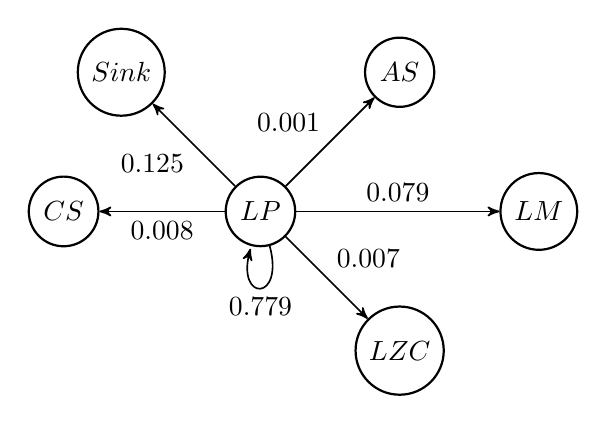
\begin{tikzpicture}[->, >=stealth', auto, semithick, node distance=2.5cm]
\tikzstyle{every state}=[fill=white,draw=black,thick,text=black,scale=1]
\node[state]    (A)                     {$LP$};
%\node[state]    (B)[above right of=A]   {$AS$};
\node[state]    (B)[above right of=A]   {$AS$};
%\node[state]    (C)[above left of=B]    {$Bl$};
%\node[state]    (D)[left of=C]          {$CS$};
\node[state]    (D)[left of=A]          {$CS$};
%\node[state]    (E)[below right of=A]   {$CC$};
%\node[state]    (F)[below left of=E]    {$LC$};
%\node[state]    (G)[below right of=B]   {$LZC$};
\node[state]    (G)[below right of=A]   {$LZC$};
%\node[state]    (H)[below right of =G]  {$LM$};
\node[state]    (H)[below right of =B]  {$LM$};
%\node[state]    (I)[below left of=H]    {$MCh$};
%\node[state]    (J)[above right of=B]   {$RP$};
%\node[state]    (K)[above right of=G]   {$SC$};
%\node[state]    (L)[above of=B]         {$SG$};
%\node[state]    (M)[below right of=K]   {$SA$};
%\node[state]    (N)[above of=D]         {$Bu$};
%\node[state]    (O)[left of=D]          {$Source$};
%\node[state]    (P)[below right of=O]   {$Cm$};
%\node[state]    (Q)[below left of=P]    {$Cp$};
%\node[state]    (R)[below left of=A]    {$FM$};
%\node[state]    (S)[above right of=K]   {$Sink$};
\node[state]    (S)[above left of=A]   {$Sink$};
%\node[state]	(V)[below left of=R]	{$De$};
%\node[state]    (U)[below right of=N]    {$Ob$};
%\node[state]    (Y)[above right of=O]   {$PT$};
%\node[state]    (Z)[below left of=O]    {$Si$};

\path
(A) edge[loop below]     node{$0.779$}   (A)
edge        node{$0.001$}       (B)
edge         node{$0.008$}      (D)
edge       node{$0.007$}        (G)
edge        node{$0.079$}       (H)
edge         node{$0.125$}      (S);

\end{tikzpicture}
}
\caption{LongParameterList (LP) mutation in ApacheSolr.}
\label{Figure:LP-Mutations-ApacheSolr}
\end{center}
\end{figure*}


\begin{figure*} %[ht]
\begin{center}
\scalebox{0.7}{
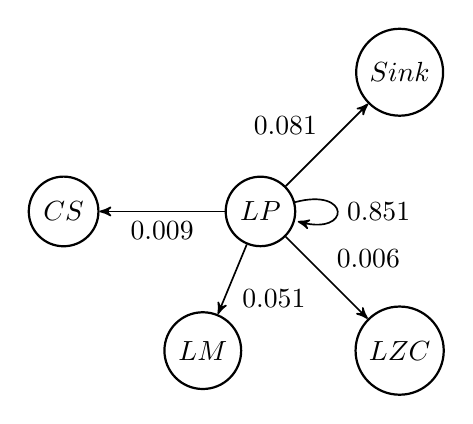
\begin{tikzpicture}[->, >=stealth', auto, semithick, node distance=2.5cm]
\tikzstyle{every state}=[fill=white,draw=black,thick,text=black,scale=1]
\node[state]    (A)                     {$LP$};
%\node[state]    (B)[above right of=A]   {$AS$};
%\node[state]    (C)[above left of=B]    {$Bl$};
%\node[state]    (D)[left of=C]          {$CS$};
\node[state]    (D)[left of=A]          {$CS$};
%\node[state]    (E)[below right of=A]   {$CC$};
%\node[state]    (F)[below left of=E]    {$LC$};
%\node[state]    (G)[below right of=B]   {$LZC$};
\node[state]    (G)[below right of=A]   {$LZC$};
%\node[state]    (H)[below right of =G]  {$LM$};
\node[state]    (H)[below right of =D]  {$LM$};
%\node[state]    (I)[below left of=H]    {$MCh$};
%\node[state]    (J)[above right of=B]   {$RP$};
%\node[state]    (K)[above right of=G]   {$SC$};
%\node[state]    (L)[above of=B]         {$SG$};
%\node[state]    (M)[below right of=K]   {$SA$};
%\node[state]    (N)[above of=D]         {$Bu$};
%\node[state]    (O)[left of=D]          {$Source$};
%\node[state]    (P)[below right of=O]   {$Cm$};
%\node[state]    (Q)[below left of=P]    {$Cp$};
%\node[state]    (R)[below left of=A]    {$FM$};
%\node[state]    (S)[above right of=K]   {$Sink$};
\node[state]    (S)[above right of=A]  {$Sink$};
%\node[state]	(V)[below left of=R]	{$De$};
%\node[state]    (U)[below right of=N]   {$Ob$};
%\node[state]    (Y)[above right of=O]   {$PT$};
%\node[state]    (Z)[below left of=O]    {$Si$};

\path
(A) edge[loop right]     node{$0.851$}   (A)
edge         node{$0.009$}      (D)
edge       node{$0.006$}        (G)
edge        node{$0.051$}       (H)
edge         node{$0.081$}      (S);

\end{tikzpicture}
}
\caption{LongParameterList (LP) mutation in ApacheIgnite.}
\label{Figure:LP-Mutations-ApacheIgnite}
\end{center}
\end{figure*}

\begin{figure}
\begin{center}
\scalebox{0.8}{
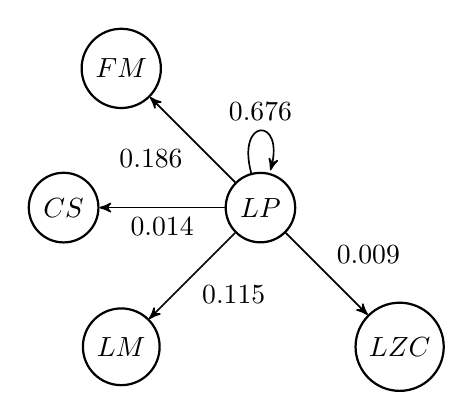
\begin{tikzpicture}[->, >=stealth', auto, semithick, node distance=2.5cm]
\tikzstyle{every state}=[fill=white,draw=black,thick,text=black,scale=1]
\node[state]    (A)                     {$LP$};
%\node[state]    (B)[above right of=A]   {$AS$};
%\node[state]    (C)[above left of=B]    {$Bl$};
%\node[state]    (D)[left of=C]          {$CS$};
\node[state]    (D)[left of=A]          {$CS$};
%\node[state]    (E)[below right of=A]   {$CC$};
%\node[state]    (F)[below left of=E]    {$LC$};
%\node[state]    (G)[below right of=B]   {$LZC$};
\node[state]    (G)[below right of=A]   {$LZC$};
%\node[state]    (H)[below right of =G]  {$LM$};
\node[state]    (H)[below left of =A]  {$LM$};
%\node[state]    (I)[below left of=H]    {$MCh$};
%\node[state]    (J)[above right of=B]   {$RP$};
%\node[state]    (K)[above right of=G]   {$SC$};
%\node[state]    (L)[above of=B]         {$SG$};
%\node[state]    (M)[below right of=K]   {$SA$};
%\node[state]    (N)[above of=D]         {$Bu$};
%\node[state]    (O)[left of=D]          {$Source$};
%\node[state]    (P)[below right of=O]   {$Cm$};
%\node[state]    (Q)[below left of=P]    {$Cp$};
%\node[state]    (R)[below left of=A]    {$FM$};
\node[state]    (R)[above left of=A]    {$FM$};
%\node[state]    (S)[above right of=K]   {$Sink$};
%\node[state]	(V)[below left of=R]	{$De$};
%\node[state]    (U)[below right of=N]    {$Ob$};
%\node[state]    (Y)[above right of=O]   {$PT$};
%\node[state]    (Z)[below left of=O]    {$Si$};

\path
(A) edge[loop above]     node{$0.676$}   (A)
%edge        node{$0.001$}       (B)
edge         node{$0.014$}      (D)
edge         node{$0.009$}      (G)
edge         node{$0.115$}      (H)
edge         node{$0.186$}      (R);

\end{tikzpicture}
}
\caption{LongParameterList (LP) mutation in Mule.}
\label{Figure:LP-Mutations-Mule}
\end{center}
\end{figure}



Tables \ref{tab:EclipseMarkov} to \ref{tab:Mulemarkov} show the mutations between design patterns and design anti-patterns that occurred in their evolutions. Table \ref{tab:AllSystems} aggregates all the mutations in all the systems. We added two additional states (source and sink) to describe the appearances of design (anti-)patterns (sources) and the disappearance of some design (anti-)patterns (sinks).

% A \textit{Source} indicates the new classes which did not participate in the occurrences of design patterns and--or design anti-patterns before the selected period of evolution. A \textit{sink}, on the other hand, represents the classes which participated in occurrences of design patterns and--or design anti-patterns during the selected period of evolution but not after.

\begin{table*} %[ht]
\centering
\caption{Standard deviation values and confidence levels}
\scalebox{0.9}{
\renewcommand{\arraystretch}{1.05}
\begin{math}
\begin{tabular}{|l|r|r|r|}
\hline
\textbf{Systems} & \textbf{Standard Deviation} & \textbf{Confidence Level} & \textbf{Margin of Error}\\
 \hline \hline
 Apache Ignite & 0.1966 & 90\%, 1.645 $\sigma x$ & 0.04347$\pm$0.0147 ($\pm$33.87\%)\\ 
 \hline
 Apache Solr & 0.1921 & 90\%, 1.645 $\sigma x$ & 0.04343$\pm$0.0144 ($\pm$33.12\%) \\
 \hline
 Eclipse & 0.1833 & 90\%, 1.645 $\sigma x$ & 0.04317$\pm$0.0137 ($\pm$31.79\%) \\
\hline
 Matsim & 0.1722 & 90\%, 1.645 $\sigma x$ & 0.04304 $\pm$0.0129 ($\pm$29.96\%) \\
\hline
 Mule & 0.1766 & 90\%, 1.645 $\sigma x$ & 0.04345 $\pm$0.0132($\pm$30.43\%) \\
\hline
 Nuxeo & 0.1968 & 90\%, 1.645 $\sigma x$ & 0.0451 $\pm$0.0147 ($\pm$32.67\%) \\
\hline
 oVirt & 0.1961 & 90\%, 1.645 $\sigma x$ & 0.04352 $\pm$0.0147 ($\pm$33.73\%) \\
\hline
\end{tabular}
\end{math}
}
\label{tab:standardDeviation}
\end{table*}

The mutation probabilities shown in previous tables are percentages that may hide outliers. Therefore, we also calculate the standard deviation values among these probabilities. 
%Low standard deviation values mean that most of the numbers are close to the average while a high standard deviation values mean that the numbers are spread out.
We found that the probabilities across snapshots have low standard-deviation values, as shown in Table \ref{tab:standardDeviation}, with the highest value of 0.196 for Nuxeo. 

% These low standard-deviation values indicate that the values shown in the tables are representative of their trends and that we can be confident in the conclusion drawn from them.

Table \ref{tab:standardDeviation} shows a systematic analysis of the confidence levels of our results. We computed the standard-deviation values and confidence intervals of our results for a confidence level of 90\% as follows:

\begin{equation}
    \sigma = \sqrt{\frac{1}{N}\sum_{i=1}^{N}{ (x_i-\mu)}^2}
\end{equation}

\noindent where $x_i$ is each value from the population (mutations probabilities), $\mu$ is the mean of the population, and $N$ is the size of the population, \ie{} the total number of mutations in all the snapshots of a system.

With the standard deviation known, we compute the confidence interval for a population mean as:

\begin{equation}
    \bar{X}\pm Z \times {\frac{\sigma}{\sqrt{N}}}
\end{equation}

\noindent where $\bar{X}$ is plus or minus a margin of error, $Z$ is the Z-value for the chosen confidence level, $\sigma$ is a standard deviation and $N$ is the size of the population.

We observe that, for a confidence level of 90\%, the confidence intervals, which indicate how much we can expect the results to reflect the observations from the overall population, were around 30\% in all the analysed systems. We consider these values of confidence levels and intervals acceptable to deduce trends and infer conclusions. Indeed, while we could not find similar discussions and numbers in other software-engineering papers, we observed similar values used to deduce trends in other domains, \eg{} public health \cite{strazzullo2009salt}.

\begin{table*} %[ht]
\centering
\caption{Mean values of the mutations of design anti-patterns and design pattern occurrences mutated in all the snapshots of each system}
\scalebox{0.8}{
\renewcommand{\arraystretch}{1.1}
\begin{math}
\begin{tabular}{|l|r|r|}
\hline
\textbf{Systems} & \textbf{Mean Value of DAPs mutations} & \textbf{Mean Value of DPs mutations} \\
 \hline \hline
 Apache Ignite & 0.0799 & 0.0037 \\ 
 \hline
 Apache Solr & 0.1026 & 0.0232 \\
 \hline
 Eclipse & 0.1355 & 0.1128 \\
\hline
 Matsim & 0.2013 & 0.1917 \\
\hline
 Mule & 0.1989 & 0.1341 \\
\hline
 Nuxeo & 0.0848 & 0.03 \\
\hline
 oVirt & 0.0674 & 0.0252 \\
\hline
\end{tabular}
\end{math}
}
\label{tab:MeanValue}
\end{table*} 

For example, SpaghettiCode has the most representative mutation probability from Source in Mule (see Table \ref{tab:Mulemarkov}) and Blob to Sink in Apache Solr (see Table \ref{tab:SolrMarkov}). Table \ref{tab:mostrp} shows the most representative design patterns and design anti-patterns regarding mutation probabilities to/from other patterns.

\begin{table*} %[ht]
\centering
\renewcommand {\arraystretch} {1.1}
\caption{Most representative mutations between design patterns and design anti-patterns according to their mutation probabilities}
\scalebox{0.7}{
\begin{tabular}{|p{1.75cm}|l|l|l|r|}
\hline
\textbf{System} & \textbf{Mutation Type} & \textbf{From}  & \textbf{To} & \textbf{Probability} \\ \hline
\hline
\multirow{4}{*}{Apache Ignite} & DAP$\,\to\,$DAP & Blob (Bl) & AntiSingleton (AS) & 0.375\\
\cline{2-5}
& DAP$\,\to\,$DP & - & - & -\\
\cline{2-5}
  & DP$\,\to\,$DAP & - & - & -\\
  \cline{2-5}
   & DP$\,\to\,$DP & Builder (Bu) & Observer (ob) & 0.004\\
  \cline{2-5}
\hline
\multirow{4}{*}{Apache Solr} & DAP$\,\to\,$DAP & Blob (Bl) & AntiSingleton (AS) & 0.321\\
\cline{2-5}
& DAP$\,\to\,$DP & - & - & -\\
\cline{2-5}
& DP$\,\to\,$DAP & - & - & -\\
\cline{2-5}
& DP$\,\to\,$DP & FactoryMethod (FM) & Composite (Cp) & 0.012\\
\hline 
\multirow{4}{*}{Eclipe IDE} & DAP$\,\to\,$DAP & LargeClass (LC) & ComplexClass (Cc) & 0.500\\
\cline{2-5}
 & DAP$\,\to\,$DP & - & - & -\\
\cline{2-5}
 & DP$\,\to\,$DAP & FactoryMethod (FM) & LongMethod (LM) & 0.003\\
\cline{2-5}
 & DP$\,\to\,$DP & FactoryMethod (FM) & Composite (Cp) & 0.169\\
\hline 
\multirow{4}{*}{Matsim} & DAP$\,\to\,$DAP & Blob (Bl) & AntiSingleton (AS) & 0.372\\
\cline{2-5}
 & DAP$\,\to\,$DP & Blob (Bl) & FactoryMethod (FM) & 0.346\\
\cline{2-5}
 & DP$\,\to\,$DAP & Command (Cm) & SwissArmyKnife (SA) & 0.030\\
\cline{2-5}
 & DP$\,\to\,$DP & Command (Cm) & FactoryMethod (FM) & 0.387\\
\hline 
\multirow{4}{*}{Mule} & DAP$\,\to\,$DAP & Blob (bl) & AntiSingleton(AS) & 0.313\\
\cline{2-5}
 & DAP$\,\to\,$DP & RefusedParentBequest (RP) & FactoryMethod (FM) & 0.433\\
\cline{2-5}
 & DP$\,\to\,$DAP & Command (Cm) & SwissArmyKnife (SA) & 0.019\\
\cline{2-5}
 & DP$\,\to\,$DP & Command (Cm) & FactoryMethod & 0.193\\
\hline 
\multirow{4}{*}{Nuxeo} & DAP$\,\to\,$DAP & Blob (bl) & AntiSingleton(AS) & 0.283\\
\cline{2-5}
 & DAP$\,\to\,$DP & Blob (Bl) & FactoryMethod (FM) & 0.297\\
\cline{2-5}
 & DP$\,\to\,$DAP & Singleton (Si) & LazyClass (ZC) & 0.004\\
\cline{2-5}
 & DP$\,\to\,$DP & Singleton (Si) & FactoryMethod (FM) & 0.133\\
\hline 
\multirow{4}{*}{ovirt} & DAP$\,\to\,$DAP & Blob (bl) & AntiSingleton(AS) & 0.299\\
\cline{2-5}
 & DAP$\,\to\,$DP & - & - & -\\
\cline{2-5}
 & DP$\,\to\,$DAP & Singleton (Si) & AntiSingleton (AS) & 0.001\\
\cline{2-5}
 & DP$\,\to\,$DP & Singleton (Si) & Prototype (PT) & 0.097\\
\hline 
\end{tabular}
}
\label{tab:mostrp}
\end{table*} 

\paragraph{\textbf{Analysing pattern evolution}} We observe in Table \ref{tab:mostrp} that not all design patterns and design anti-pattern undergo changes. Some patterns remain stable during evolution. For example, LazyClass and MessageChain are stable design anti-patterns, while Prototype is a persistent design pattern in Apache Solr. In Matsim, design anti-patterns SwissArmyKnife, LazyClass, and MessageChain and design patterns Observer and ProtoType are stable.

However, in general, design anti-patterns tend to evolve in all studied systems. We observe that more than half of the design anti-patterns mutated into other design patterns or design anti-patterns across the different snapshots of the studied system. 

For example, in Matsim (see Table \ref{tab:MatsimMarkov}), 86\% (probability value 0.86) LongMethod remains stable and mutate with only a probability of 14\% into other patterns. In oVirt (see Table \ref{tab:Ovirtmarkov}), Blob remain persistent in the system with 39.4\% probability, while 29.9\% mutated to AntiSingleton and into other patterns with a probability of 30.8\%. As last example, in Eclipse, 45.5\% of RefusedParentBequest remain between snapshot while 27.3\% mutated to MessageChain and 27.3\% mutated into other patterns.

We saw fewer mutations among design patterns. As an example, in Apache Ignite, 97.6\% of Command remained stable, with only 0.4\% mutating into other patterns.

% In general, we believe that mutations happen when developers solve design and coding problems. They modify the code and--or apply design patterns to these problems. Yet, they can also introduce design anti-patterns or other, undesired design pattern.

% We built Markov models to compute the probabilities of design anti-patterns and design patterns appearing, disappearing, and mutating during software evolution. We studied seven systems with different sizes to generalize our findings.

For a better understanding of the design pattern and design anti-pattern mutations, Figures \ref{Figure:FM-Mutations-Eclipse} to \ref{Figure:LP-Mutations-Mule} show the most representative mutations in the Markov models as graphs, for each of the systems. Because showing all possible probabilities would make the graphs unreadable, we choose a threshold of 0.100 to reduce the number of edges in each graph. The gray cells in Tables \ref{tab:EclipseMarkov} to  \ref{tab:Mulemarkov} highlight the probabilities shown in the figures. (The graphs for all the mutations in all the systems are available on-line\footnote{\url{http://www.ptidej.net/downloads/replications/emse19c/}}.)

These graphs contain information on mutating design (anti-)patterns that can help developers to avoid the mutations that could have negative impacts on software quality. 

\begin{tcolorbox}
\vspace{-0.1cm}
\textbf{Summary:} Our results show that design patterns and design anti-patterns mutate during the evolution of software systems. Despite an average of less than 20\% of the identified design anti-patterns occurrences having mutated among all the snapshots of systems, more than half of the types of design anti-patterns were involved in these mutations. For example, Table \ref{tab:MeanValue} shows that, in Matsim, 20.13\% of the design anti-pattern identified  in the first snapshot mutated during the studied period. During that period, ten types of design anti-patterns out of the 13 considered in our study were involved in mutations. In most of the systems, almost all the design patterns remained stable during evolution. Blob and Command are the design anti-patterns and design pattern with the higher mutation probabilities.
\vspace{-0.1cm}
\end{tcolorbox}



\subsection{\textbf{RQ2:} \textit{\RQTwo}}

\paragraph{\textbf{Motivation}} Knowing the causes of design (anti-)patterns mutations would be useful during maintenance. They could help developers to focus on the most frequent change types triggering patterns mutations. 

% Thus, we identify the types of changes to understand why and how design patterns and--or design anti-patterns mutate between two successive snapshots.  

\paragraph{\textbf{Analysing change types}} We use srcML\footnote{https://www.srcml.org/} to create an XML file for each snapshot of a system and match their tags to find changed tags, as explained in Section \ref{ssec:section3.6}. We categorise change types based on our categories in Table \ref{tab:Change_types}. We compare the percentages of each change type for each system. We apply the same methodology for all the subject systems.
Figures \ref{fig:FigureChangeEclipseNew} to \ref{fig:FigureChangeMuleNew} show the types of changes per design (anti-)patterns per systems. 

Table \ref{tab:Changes} presents the numbers of each change types in all the systems. For example, in Apache Ignite, we observe that Access and  Renaming are the least and most representative change types for both design patterns and design anti-patterns. They lead to many changes in occurrences of both design anti-patterns and design patterns.

\begin{landscape}
\begin{center}
	\begin{table*}
		\renewcommand {\arraystretch} {1.05}
		\centering
		
		\caption{Number of different types of changes in design patterns and design anti-patterns\label{tab:Changes}}
		\scalebox{0.61}{
		%\begin{tabular}{|p{2.05cm}|p{0.55cm}|p{0.55cm}|p{0.6cm}|p{0.4cm}|p{0.7cm}|p{0.4cm}|p{0.7cm}|p{0.7cm}|p{0.55cm}|p{0.45cm}|p{0.55cm}|p{0.35cm}|p{0.55cm}|p{0.55cm}|} \hline
		\begin{tabular}{|p{2.7cm}|r|r|r|r|r|r|r|r|r|r|r|r|r|r|} \hline
			\textbf{Systems~$\rightarrow$} & \multicolumn{2}{c}{\textbf{Eclipse}}& \multicolumn{2}{|c}{\textbf{Nuxeo}} & \multicolumn{2}{|c}{\textbf{oVirt}}& \multicolumn{2}{|c}{\textbf{Matsim}}&\multicolumn{2}{|c}{\textbf{Apache Solr}}&\multicolumn{2}{|c}{\textbf{Apache Ignite}}&\multicolumn{2}{|c|}{\textbf{Mule}}\\ \hline 
			\multirow{2}{*}{\textbf{Change Types~$\downarrow$}}
			& 1~~~ & 2~~~ & 3~~~ & 4~~~ & 5~~~ & 6~~~ & 7~~~ & 8~~~ & 9~~~ & 10~~ & 11~~ & 12~~ & 13~~ & 14~~\\ \cline{2-15} 
			& \textbf{DAP}~~ & \textbf{DP}~~ & \textbf{DAP}~~ & \textbf{DP}~~  & \textbf{DAP}~~ & \textbf{DP}~~ & \textbf{DAP}~~ & \textbf{DP}~~ & \textbf{DAP}~~ & \textbf{DP}~~ & \textbf{DAP}~~ & \textbf{DP}~~ & \textbf{DAP}~~ & \textbf{DP}~~\\ \hline \hline
			Access & 33 & 6 & 85 & 0 & 174 & 9 & 271 & 117 & 34	& 15 & 11 & 55 & 20&12	\\ \hline
			Class & 268 & 91 & 236 & 6 & 3804 & 90 & 1697 &	690 & 721 & 155 & 781&218 & 443&198 \\ \hline
			Code block & 4197 &	1075 & 1070	& 13 & 13923 &	233 & 8805 & 3203 &	3873 & 459 & 3903&203 &1430 &413	\\ \hline 
			Comment & 32939 & 11388	& 9269	& 109 &	15013 &	411 & 22519	& 9287 & 9298 &	2616 & 14554& 1567& 6354&3780	\\ \hline 
			Control Flow & 10487 & 1870	& 966 &	10 & 6440 &	118 & 5398	& 2094 & 3166 & 636 & 3433 & 133 &916 &384	\\ \hline 
			Declaration & 9721 & 2789 &	3133 & 24 &	 27605 & 487 & 24244 & 9609 & 8803 & 1392 & 9527& 349 &3904 &1103	\\ \hline 
			Exception & 996 & 341 &	946 & 1	& 619 &	29 & 1602 &	314 & 1696 & 457 & 2076& 64& 505&173	    \\ \hline
			Import & 2566 &	835 & 2734	& 23 & 18819 & 211 & 13013 & 4679 &	4024 & 491 & 4584& 394&3234 &793	    \\ \hline
			Invocation & 1707 & 394	& 556 & 4 & 7312 & 91 &	8520 & 3026	& 2598	& 287 & 2069 & 75 &945 &240	    \\ \hline
			Method & 4060 &	942 & 1487	& 29 & 13792 & 292 & 4702 &	1922 & 3215	& 511 & 3364 & 266 & 1940&747	\\ \hline 
			Operator & 13540 & 2803	& 3533	& 8	& 35513	& 403 &	57112 &	24326 &	7963 & 702 & 7207& 525& 5241&1975	\\ \hline 
			Parameter & 5629 & 1541	& 2179	& 3 & 24488	& 292 &	22080 &	5149 & 8375 & 1069  & 9024& 332&3252 &756	\\ \hline 
			Renaming & 59254 & 14707 & 16259 & 23 &	262491 &3536 &294661&145720& 44422 & 4811 & 63961& 4396&28110&9738	\\ \hline 
			\textbf{\#Changed classes} & 10957 & 3155 & 5402& 81 & 34780 & 55 & 32596 & 13768 & 7956& 1192 & 9290& 857& 5684&2175	\\ \hline
			\textbf{Total classes} & 20331 &	7574 &	39051 &	1263 & 142537 & 2482 & 62272 & 79480 & 32332 & 5490 & 27080 & 5796 & 47146&17553	\\ \hline
			\multicolumn{15}{c}{\textbf{AP, DP}= Number of changes in design anti-patterns and design patterns respectively}\\ \hline	
		\end{tabular}
		}
	\end{table*}
	
	\begin{table*}
		\centering
		\renewcommand {\arraystretch} {1.05}
		\caption{Number of different types of changes in design patterns and design anti-patterns mutation.\label{tab:dpapMutations}}
		%\begin{tabular}{|p{2cm}|p{0.57cm}|p{0.57cm}|p{0.57cm}|p{0.57cm}|p{0.57cm}|p{0.57cm}|p{0.57cm}|p{0.57cm}|p{0.57cm}|p{0.57cm}|p{0.57cm}|p{0.57cm}|p{0.57cm}|p{0.57cm}|} \hline
		%	Systems$\rightarrow$ & \multicolumn{2}{c}{Eclipse}& \multicolumn{2}{|c}{Nuxeo} & \multicolumn{2}{|c}{Ovirt}& \multicolumn{2}{|c}{Matsim}&\multicolumn{2}{|c|}{Apache Solr}&\multicolumn{2}{|c|}{Apache Ignite}&\multicolumn{2}{|c|}{Mule}\\ \hline 
		%	\multirow{2}{*}{Change Types~$\downarrow$}
		%	& 1 & 2 & 3 & 4 & 5 & 6 & 7 & 8 & 9 & 10 & 11 & 12& 13 & 14\\ \cline{2-15}
		\scalebox{0.58}{
		\begin{tabular}{|p{2.5cm}|r|r|r|r|r|r|r|r|r|r|r|r|r|r|} \hline
			\textbf{Systems$\rightarrow$} & \multicolumn{2}{c}{\textbf{Eclipse}}& \multicolumn{2}{|c}{\textbf{Nuxeo}} & \multicolumn{2}{|c}{\textbf{oVirt}}& \multicolumn{2}{|c}{\textbf{Matsim}}&\multicolumn{2}{|c}{\textbf{Apache Solr}}&\multicolumn{2}{|c}{\textbf{Apache Ignite}}&\multicolumn{2}{|c|}{\textbf{Mule}}\\ \hline 
			\multirow{2}{*}{\textbf{Change Types~$\downarrow$}}
			& 1~~~~ & 2~~~~ & 3~~~~ & 4~~~~ & 5~~~~ & 6~~~~ & 7~~~~ & 8~~~~ & 9~~~~ & 10~~~ & 11~~~ & 12~~~ & 13~~~ & 14~~~\\ \cline{2-15} 
			 & \textbf{APDP} & \textbf{DPAP} & \textbf{APDP} & \textbf{DPAP} & \textbf{APDP} & \textbf{DPAP} & \textbf{APDP} & \textbf{DPAP} & \textbf{APDP} & \textbf{DPAP} & \textbf{APDP} & \textbf{DPAP} & \textbf{APDP} & \textbf{DPAP}\\ \hline \hline
			Access & 0 & 0 &0 & 1 &1 &1 &0 &12 &3 &0 &0 &0 &0 &1	\\ \hline
			Class & 3&1	&2	&0	&10	&0	&4 &29	&1	&7 &2 &4 &6 &3 \\ \hline
			Code block & 1 &2 &1 &4	&21	&22	&10	&132 &4	&1 &1 &3 &27 &17	\\ \hline 
			Comment & 102&192	&7	&4	&69	&31	&38	&739 &129 &242 &58 &23 &160 &85	\\ \hline 
			Control Flow & 28&38&0	&3	&7	&6	&12	&96	&44	&31	 &16 &4 &21 &3	\\ \hline 
			Declaration & 56 & 78 & 3 &2 &82 &38 &56 &412 &141 &90 &33 &16 &49 &32	\\ \hline 
			Exception & 4&6	&0	&0	&4	&1	&6	&28	&19	&13	&14 &4 &3 &2	    \\ \hline
			Import & 20&14	&3 &2	&32	&18	&28	&257 &60 &34 &17 &16 &28 &18	    \\ \hline
			Invocation & 6&	7&0	&0	&15	&20	&7	&183 &1	&6	&5 &6 & 10&3	    \\ \hline
			Method & 16&18	&2	&2	&41	&24	&7	&96	&64	&43	 &10 &12 &23 &13	\\ \hline 
			Operator & 38&37 &2	&0	&43	&66	&95	&523 &22 &20 &6 &13 &87 &32	\\ \hline 		
			Parameter & 22 & 41 & 0 & 0	&37	&20	&16	&423 &25 &47 &22 &29 &13 &22	\\ \hline 
			Renaming & 675&	469&3 &2 &297 &1036	&462 &5096	&165 &406 &100 &63 &334 &280	\\ \hline 
			\#Changed classes& 71 & 77 & 7 & 6	& 61 & 54 &58 &681 &58	&66	 &34 &29 &53 &39	\\ \hline
			\multicolumn{15}{c}{\textbf{APDP, DPAP}= Number of changes in design anti-patterns to design patterns and design patterns to design anti-patterns mutations respectively}\\ \hline
		\end{tabular}
		}
	\end{table*}
\end{center}
\end{landscape}

% Eclipse
\begin{figure}
\centering
\scalebox{1.1}{
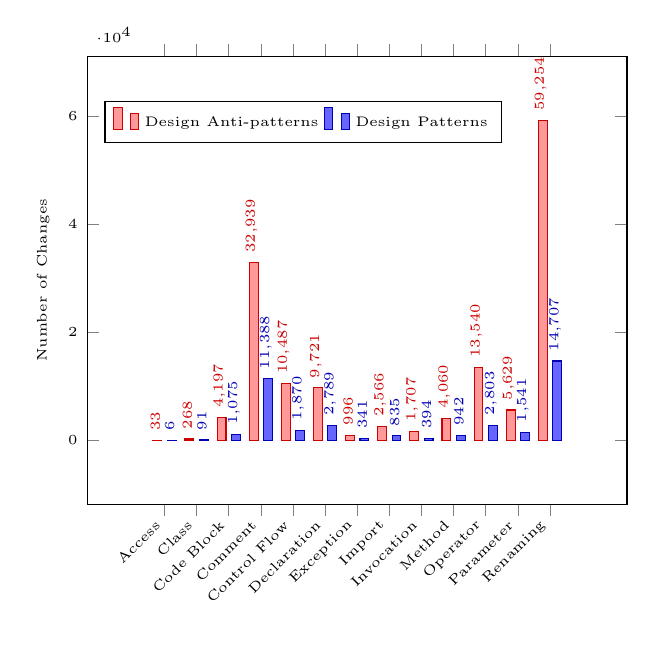
\begin{tikzpicture}
\pgfplotsset{every node/.append style={font=\tiny}}
\pgfplotsset{every tick label/.append style={font=\tiny}}
\begin{axis}[
    ybar,
    ymin=0,
    enlargelimits=0.2,
    legend style={at={(0.4,0.9)},anchor=north,legend columns=-1},
    bar width=1.12mm,
    ylabel={Number of Changes},
    symbolic x coords={Access, Class, Code Block, Comment, 
		Control Flow, Declaration, Exception, Import, Invocation, Method, Operator, Parameter, Renaming},
    xtick=data,
    x tick label style={rotate=45,anchor=east},
    nodes near coords,
    nodes near coords align={center},style={font=\tiny},
    every node near coord/.append style={rotate=90,anchor=south west,
    inner ysep=-1.75pt,}
    ]

\addplot [red!80!black,fill=red!40] coordinates {
(Access,33)
(Class,268) 
(Code Block,4197)
(Comment,32939)
(Control Flow,10487)
(Declaration,9721)
(Exception,996)
(Import,2566)
(Invocation,1707)
(Method,4060)
(Operator,13540)
(Parameter,5629)
(Renaming,59254)};
  
\addplot [blue!70!black,fill=blue!60] coordinates {
(Access,6) 
(Class,91)
(Code Block,1075) 
(Comment,11388)
(Control Flow,1870)
(Declaration,2789)
(Exception,341)
(Import,835)
(Invocation,394)
(Method,942)
(Operator,2803)
(Parameter,1541)
(Renaming,14707)};
\legend{Design Anti-patterns, Design Patterns}
\end{axis}
\end{tikzpicture}
}
\caption{Number of different types of changes in Eclipse classes with design anti-patterns and design patterns.}
\label{fig:FigureChangeEclipseNew}
\end{figure}

% Nuxeo
\begin{figure}
\centering
\scalebox{1.1}{
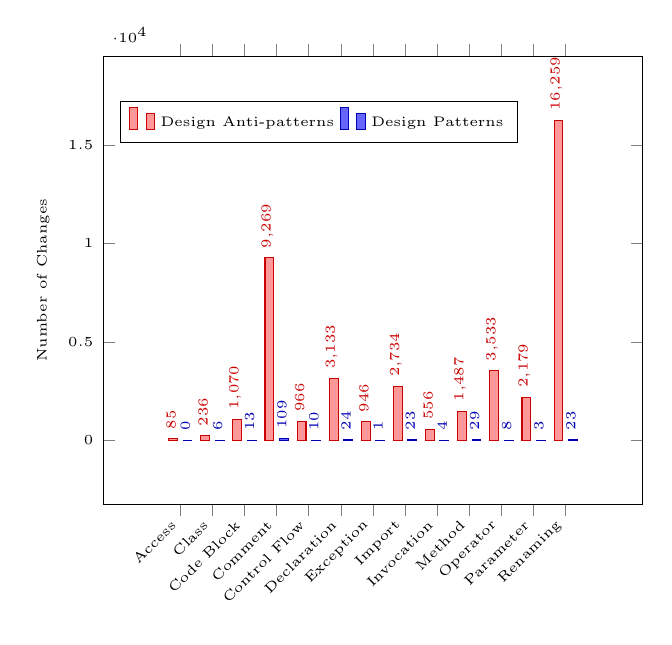
\begin{tikzpicture}
\pgfplotsset{every node/.append style={font=\tiny}}
\pgfplotsset{every tick label/.append style={font=\tiny}}
\begin{axis}[
    ybar,
    ymin=0,
    enlargelimits=0.2,
    legend style={at={(0.4,0.9)},anchor=north,legend columns=-1},
    bar width=1.12mm,
    ylabel={Number of Changes},
    symbolic x coords={Access, Class, Code Block, Comment, 
		Control Flow, Declaration, Exception, Import, Invocation, Method, Operator, Parameter, Renaming},
    xtick=data,
    x tick label style={rotate=45,anchor=east},
    nodes near coords,
    nodes near coords align={center},style={font=\tiny},
    every node near coord/.append style={rotate=90,anchor=south west,
    inner ysep=-1.75pt,}
    ]

\addplot [red!80!black,fill=red!40] coordinates {
(Access,85)
(Class,236) 
(Code Block,1070)
(Comment,9269)
(Control Flow,966)
(Declaration,3133)
(Exception,946)
(Import,2734)
(Invocation,556)
(Method,1487)
(Operator,3533)
(Parameter,2179)
(Renaming,16259)};
  
\addplot [blue!70!black,fill=blue!60] coordinates {
(Access,0) 
(Class,6)
(Code Block,13) 
(Comment,109)
(Control Flow,10)
(Declaration,24)
(Exception,1)
(Import,23)
(Invocation,4)
(Method,29)
(Operator,8)
(Parameter,3)
(Renaming,23)};
\legend{Design Anti-patterns, Design Patterns}
\end{axis}
\end{tikzpicture}
}
\caption{Number of different types of changes in Nuxeo classes with design anti-patterns and design patterns.}
\label{fig:FigureChangeNuxeoNew}
\end{figure}

% Ovirt
\begin{figure}
\centering
\scalebox{1.1}{
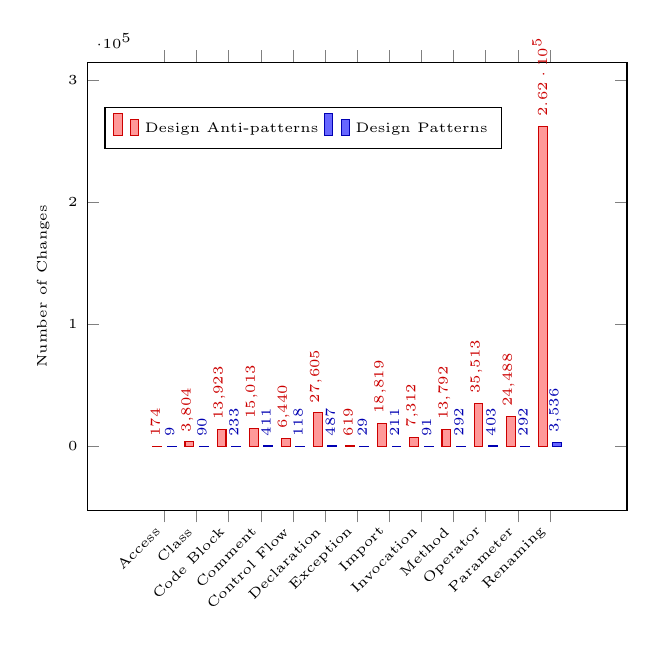
\begin{tikzpicture}
\pgfplotsset{every node/.append style={font=\tiny}}
\pgfplotsset{every tick label/.append style={font=\tiny}}
\begin{axis}[
    ybar,
    ymin=0,
    enlargelimits=0.2,
    legend style={at={(0.4,0.9)},anchor=north,legend columns=-1},
    bar width=1.12mm,
    ylabel={Number of Changes},
    symbolic x coords={Access, Class, Code Block, Comment, 
		Control Flow, Declaration, Exception, Import, Invocation, Method, Operator, Parameter, Renaming},
    xtick=data,
    x tick label style={rotate=45,anchor=east},
    nodes near coords,
    nodes near coords align={center},style={font=\tiny},
    every node near coord/.append style={rotate=90,anchor=south west,
    inner ysep=-1.75pt,}
    ]

\addplot [red!80!black,fill=red!40] coordinates {
(Access,174)
(Class,3804) 
(Code Block,13923)
(Comment,15013)
(Control Flow,6440)
(Declaration,27605)
(Exception,619)
(Import,18819)
(Invocation,7312)
(Method,13792)
(Operator,35513)
(Parameter,24488)
(Renaming,262491)};
  
\addplot [blue!70!black,fill=blue!60] coordinates {
(Access,9) 
(Class,90)
(Code Block,233) 
(Comment,411)
(Control Flow,118)
(Declaration,487)
(Exception,29)
(Import,211)
(Invocation,91)
(Method,292)
(Operator,403)
(Parameter,292)
(Renaming,3536)};
\legend{Design Anti-patterns, Design Patterns}
\end{axis}
\end{tikzpicture}
}
\caption{Number of different types of changes in oVirt classes with design anti-patterns and design patterns.}
\label{fig:FigureChangeoVirtNew}
\end{figure}

% Matsim
\begin{figure}
\centering
\scalebox{1.1}{
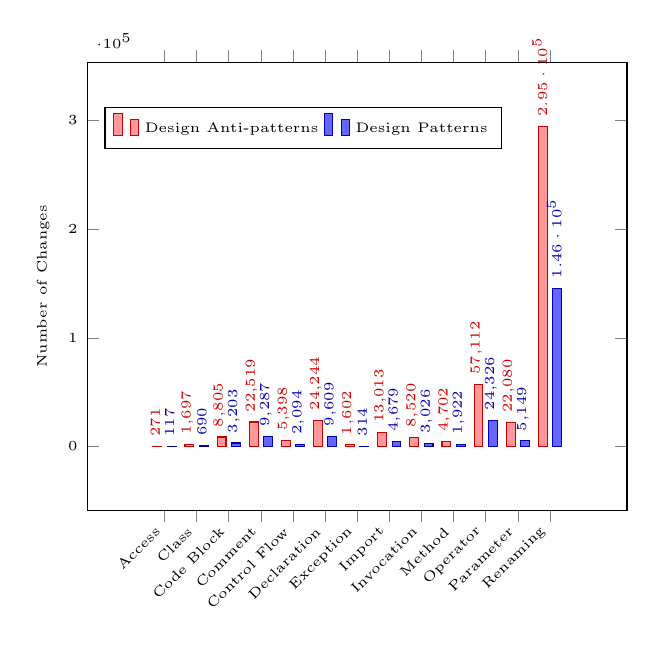
\begin{tikzpicture}
\pgfplotsset{every node/.append style={font=\tiny}}
\pgfplotsset{every tick label/.append style={font=\tiny}}
\begin{axis}[
    ybar,
    ymin=0,
    enlargelimits=0.2,
    legend style={at={(0.4,0.9)},anchor=north,legend columns=-1},
    bar width=1.12mm,
    ylabel={Number of Changes},
    symbolic x coords={Access, Class, Code Block, Comment, 
		Control Flow, Declaration, Exception, Import, Invocation, Method, Operator, Parameter, Renaming},
    xtick=data,
    x tick label style={rotate=45,anchor=east},
    nodes near coords,
    nodes near coords align={center},style={font=\tiny},
    every node near coord/.append style={rotate=90,anchor=south west,
    inner ysep=-1.75pt,}
    ]

\addplot [red!80!black,fill=red!40] coordinates {
(Access,271)
(Class,1697) 
(Code Block,8805)
(Comment,22519)
(Control Flow,5398)
(Declaration,24244)
(Exception,1602)
(Import,13013)
(Invocation,8520)
(Method,4702)
(Operator,57112)
(Parameter,22080)
(Renaming,294661)};
  
\addplot [blue!70!black,fill=blue!60] coordinates {
(Access,117) 
(Class,690)
(Code Block,3203) 
(Comment,9287)
(Control Flow,2094)
(Declaration,9609)
(Exception,314)
(Import,4679)
(Invocation,3026)
(Method,1922)
(Operator,24326)
(Parameter,5149)
(Renaming,145720)};
\legend{Design Anti-patterns, Design Patterns}
\end{axis}
\end{tikzpicture}
}
\caption{Number of different types of changes in Matsim classes with design anti-patterns and design patterns.}
\label{fig:FigureChangeMatsimNew}
\end{figure}

%ApacheIgnite
\begin{figure}
\centering
\scalebox{1.1}{
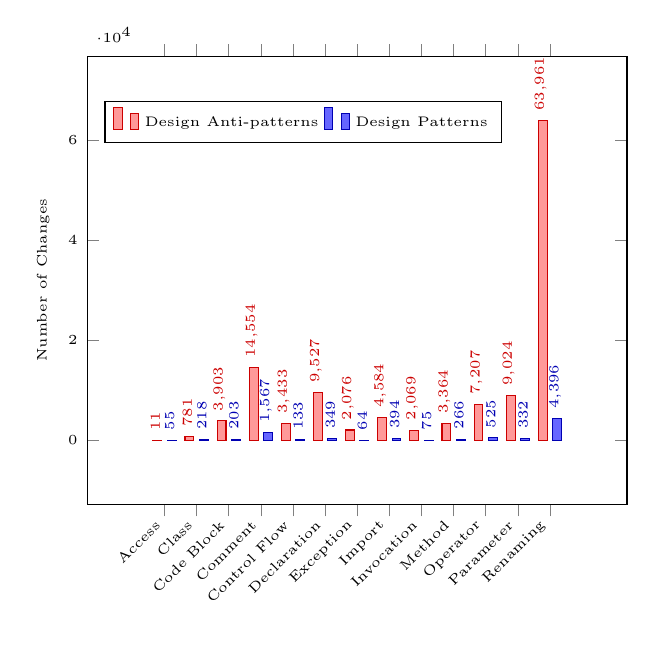
\begin{tikzpicture}
\pgfplotsset{every node/.append style={font=\tiny}}
\pgfplotsset{every tick label/.append style={font=\tiny}}
\begin{axis}[
    ybar,
    ymin=0,
    enlargelimits=0.2,
    legend style={at={(0.4,0.9)},anchor=north,legend columns=-1},
    bar width=1.12mm,
    ylabel={Number of Changes},
    symbolic x coords={Access, Class, Code Block, Comment, 
		Control Flow, Declaration, Exception, Import, Invocation, Method, Operator, Parameter, Renaming},
    xtick=data,
    x tick label style={rotate=45,anchor=east},
    nodes near coords,
    nodes near coords align={center},style={font=\tiny},
    every node near coord/.append style={rotate=90,anchor=south west,
    inner ysep=-1.75pt,}
    ]

\addplot [red!80!black,fill=red!40] coordinates {
(Access,11)
(Class,781) 
(Code Block,3903)
(Comment,14554)
(Control Flow,3433)
(Declaration,9527)
(Exception,2076)
(Import,4584)
(Invocation,2069)
(Method,3364)
(Operator,7207)
(Parameter,9024)
(Renaming,63961)};
  
\addplot [blue!70!black,fill=blue!60] coordinates {
(Access,55) 
(Class,218)
(Code Block,203) 
(Comment,1567)
(Control Flow,133)
(Declaration,349)
(Exception,64)
(Import,394)
(Invocation,75)
(Method,266)
(Operator,525)
(Parameter,332)
(Renaming,4396)};
\legend{Design Anti-patterns, Design Patterns}
\end{axis}
\end{tikzpicture}
}
\caption{Number of different types of changes in Apache Ignite classes with design anti-patterns and design patterns.}
\label{fig:FigureChangeApacheIgniteNew}
\end{figure}

%ApacheISolr
\begin{figure}
\centering
\scalebox{1.1}{
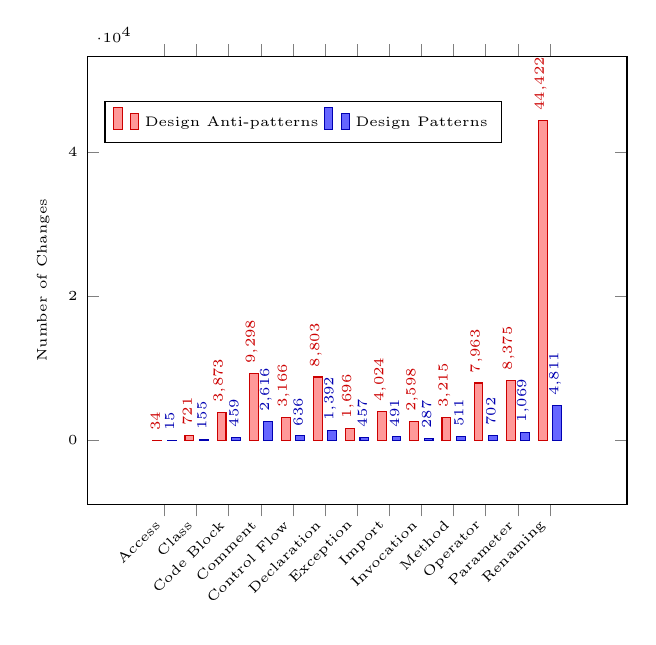
\begin{tikzpicture}
\pgfplotsset{every node/.append style={font=\tiny}}
\pgfplotsset{every tick label/.append style={font=\tiny}}
\begin{axis}[
    ybar,
    ymin=0,
    enlargelimits=0.2,
    legend style={at={(0.4,0.9)},anchor=north,legend columns=-1},
    bar width=1.12mm,
    ylabel={Number of Changes},
    symbolic x coords={Access, Class, Code Block, Comment, 
		Control Flow, Declaration, Exception, Import, Invocation, Method, Operator, Parameter, Renaming},
    xtick=data,
    x tick label style={rotate=45,anchor=east},
    nodes near coords,
    nodes near coords align={center},style={font=\tiny},
    every node near coord/.append style={rotate=90,anchor=south west,
    inner ysep=-1.75pt,}
    ]

\addplot [red!80!black,fill=red!40] coordinates {
(Access,34)
(Class,721) 
(Code Block,3873)
(Comment,9298)
(Control Flow,3166)
(Declaration,8803)
(Exception,1696)
(Import,4024)
(Invocation,2598)
(Method,3215)
(Operator,7963)
(Parameter,8375)
(Renaming,44422)};
  
\addplot [blue!70!black,fill=blue!60] coordinates {
(Access,15) 
(Class,155)
(Code Block,459) 
(Comment,2616)
(Control Flow,636)
(Declaration,1392)
(Exception,457)
(Import,491)
(Invocation,287)
(Method,511)
(Operator,702)
(Parameter,1069)
(Renaming,4811)};
\legend{Design Anti-patterns, Design Patterns}
\end{axis}
\end{tikzpicture}
}
\caption{Number of different types of changes in Apache Solr classes with design anti-patterns and design patterns.}
\label{fig:FigureChangeApacheSolrNew}
\end{figure}

% Mule
\begin{figure}
\centering
\scalebox{1.1}{
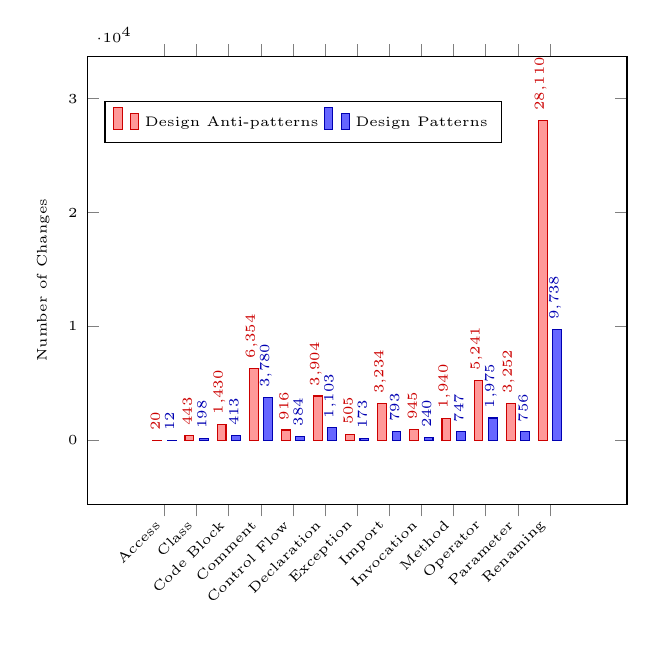
\begin{tikzpicture}
% \pgfplotsset{width = 10cm}
\pgfplotsset{every node/.append style={font=\tiny}}
\pgfplotsset{every tick label/.append style={font=\tiny}}
\begin{axis}[
    ybar,
    ymin=0,
    enlargelimits=0.2,
    legend style={at={(0.4,0.9)},anchor=north,legend columns=-1},
    bar width=1.12mm,
    ylabel={Number of Changes},
    symbolic x coords={Access, Class, Code Block, Comment, 
		Control Flow, Declaration, Exception, Import, Invocation, Method, Operator, Parameter, Renaming},
    xtick=data,
    x tick label style={rotate=45,anchor=east},
    nodes near coords,
    nodes near coords align={center},style={font=\tiny},
    every node near coord/.append style={rotate=90,anchor=south west,
    inner ysep=-1.75pt,}
    ]

\addplot [red!80!black,fill=red!40] coordinates {
(Access,20)
(Class,443) 
(Code Block,1430)
(Comment,6354)
(Control Flow,916)
(Declaration,3904)
(Exception,505)
(Import,3234)
(Invocation,945)
(Method,1940)
(Operator,5241)
(Parameter,3252)
(Renaming,28110)};
  
\addplot [blue!70!black,fill=blue!60] coordinates {
(Access,12) 
(Class,198)
(Code Block,413) 
(Comment,3780)
(Control Flow,384)
(Declaration,1103)
(Exception,173)
(Import,793)
(Invocation,240)
(Method,747)
(Operator,1975)
(Parameter,756)
(Renaming,9738)};
\legend{Design Anti-patterns, Design Patterns}
\end{axis}
\end{tikzpicture}
}
\caption{Number of different types of changes in Mule classes with design anti-patterns and design patterns.}
\label{fig:FigureChangeMuleNew}
\end{figure}

\paragraph{\textbf{Analysing change types of mutations}} During evolution, design patterns and design anti-patterns can mutate into other design patterns and design anti-patterns. We investigate which types of changes lead to such mutations. 
% The results of detected change types are contained in CSV files related to changed classes participating in design patterns and design anti-patterns for each system. Each CSV file includes the name of the two subsequent snapshots compared for change detection, the type of changes and the names of the classes changed. We compare two CSV files related to design patterns and design anti-patterns. By comparing the names of classes participating in occurrences of design patterns and design anti-patterns, we find the same class names which indicate that we have a mutation from design anti-patterns to design patterns and vice versa. 
Tables \ref{tab:dpapMutations} shows the number of each change types during the mutation for all the studied systems.

Results show that, in Apache Ignite, Renaming, Comment, and Declaration lead the most mutations from design anti-patterns (DAPs) to design patterns (DPs). It is almost the same for DPs-to-DAPs mutations but Parameter has more importance than Declaration. In Apache Solr and Eclipse for both DAPs-to-DPs and DPs-to-DAPs mutations, Renaming, Declaration, and Comment are the most representative change types. In Matsim, Renaming, Operator, and Declaration have the most impact on DAPs-to-DPs mutations while Renaming, Comment, and Operator lead to more DPs-to-DAPs mutations. In Mule, for both DAPs-to-DPs and DPs-to-DAPs mutations, Renaming, Comment, and Operator are the most representative change types. In Nuxeo, there are few mutations, in which Comment, Renaming, and Declaration yield DAPs-to-DPs mutations while Comment, Code Block, and Control Flow yield more DPs-to-DAPs mutations. Finally, in oVirt, Renaming, Declaration, and Comment are change types that lead to DAPs-to-DPs mutations while Renaming, Operator, and Declaration bring DPs-to-DAPs mutations.

Renaming is the most frequent change type. There are different types of renaming, described in \cite{arnaoudova2014repent}. In some types, an entity, \eg{} a package, a class, etc., is renamed. In other types, one or more terms are changed (simple and complex renaming). Sometimes, when one or more terms change, the meaning of the identifier also changes (semantic renaming). The grammar of an identifier may also change during evolution (grammar renaming). When developers use some tools to apply a renaming operation, the tool may not rename all variables consistently in all related files. Besides, certain source-code changes must be made together to preserve consistency. Changes in comments and declarations led to more mutations not as root causes of these mutations but because developers changed comments and declarations while evolving their systems for other reasons, \ie{} fixing faults. Future work include a manual, qualitative analysis of the mutations to identify their root causes.

\begin{tcolorbox}
\vspace{-0.1cm}
\textbf{Summary:} \emph{Some change types affect the mutations between design patterns and--or design anti-patterns more than others. We observe that the change types leading to mutations in all the studied systems are Renaming, Comment, Declaration, and Operator.}
\vspace{-0.1cm}
\end{tcolorbox}



\subsection{\textbf{RQ3:} \textit{\RQThree}}

\paragraph{\textbf{Motivation}} The results from RQ1 and RQ2 show that design patterns and design anti-patterns mutate during software evolution. However, they do not say anything about the impact of these mutations in software quality. Therefore, we investigate these mutations and their fault-proneness. Using this information, developers could understand the reasons of faults and take actions to reduce the risk of introducing faults.

\paragraph{\textbf{Analysing design patterns and design anti-patterns fault-proneness}} For each system, we mine its commit log and extract fault and commit IDs related to the faults and the dates when the faults were introduced. We look for faults introduced from one snapshot to the next. We use the dates to distinguish between faults appearing in one snapshot and those appearing between two extracted snapshots.

Table \ref{tab:DAP-DPfault} shows the numbers of faulty and clean of classes involved in patterns. One class can be involved in several faults in the studied snapshots so we show in Table \ref{tab:fault} the numbers of unique faulty and clean classes involved in patterns. Finally, in Table \ref{tab:faultpercentages}, we compare the percentages of faulty and clean classes involved in design patterns and design anti-patterns. Moreover, we show in Table \ref{tab:faultpercentages} the relative percentages of faults per class participating, or not, in design (anti-)patterns. 

With these tables, we summarise our whole dataset with: the numbers of (unique) faulty and non-faulty (clean) classes participating or not in design (anti-)patterns and their relative percentages. We thus can compare the prevalence of faults in different classes and confirm that classes participating in design anti-patterns have more faults than classes involved in design patterns. Thus, we have evidence supporting that classes that participate in design anti-patterns are more fault-prone than classes involved in design patterns.

For example, in Eclipse, 13.7\% of design pattern classes are fault-prone while 37.3\% of design anti-pattern classes are fault-prone. Table \ref{tab:faultpercentages} is showing similar trends in all the analysed systems.

\begin{table*} [ht]
\centering
\caption{Design anti-pattern and design-pattern mutations between faulty and clean classes}
\scalebox{0.8}{
\renewcommand{\arraystretch}{1.1}
\begin{tabular}{|l|r|r|r|}
\hline
\multirow{2}{*}{\textbf{\textbf{Systems}}} & \multicolumn{2}{c|}{\textbf{\# of Faulty classes}} & \multirow{2}{*}{\textbf{\# of Clean classes having DAPs, DPs}} \\
\cline{2-3}
 & Design Anti-patterns & Design Patterns & \\
 \hline \hline
 Apache Ignite & 10,984 & 1,051 & 81,093\\ 
 \hline
 Apache Solr & 11,156 & 219 & 109,225 \\
 \hline
 Eclipse & 15,240 & 5,182 & 19,928 \\
\hline
 Matsim & 4,053 & 1,888 & 896,510 \\
\hline
 Mule & 17,794 & 5,924 & 197,574 \\
\hline
 Nuxeo & 18,724 & 396 & 146,180 \\
\hline
 oVirt & 12,605 & 110 & 217,565 \\
\hline
\end{tabular}
}
\label{tab:DAP-DPfault}
\end{table*} 

\begin{table*} [ht]
\centering
\caption{Faulty and clean classes}
\scalebox{0.7}{
\renewcommand{\arraystretch}{1.1}
\begin{tabular}{|l|rr|rr|rr|rr|rr|}
\hline
\multirow{2}{*}{\textbf{Systems}} & \multicolumn{4}{c|}{\textbf{\# of Faulty Classes}} & \multicolumn{2}{c|}{\textbf{\# of Faulty Classes}} & \multicolumn{4}{c|}{\textbf{\# of Clean Classes}} \\
\cline{2-11}
& \multicolumn{2}{c|}{DAPs} & \multicolumn{2}{c|}{DPs} & \multicolumn{2}{c|}{\textbf{without Patterns}} & \multicolumn{2}{c|}{DAPs} &
\multicolumn{2}{c|}{DPs} \\
\hline \hline
Apache Ignite & 10,984 & (685) & 1,051 & (84) & 3,984 & (3,984) & 71,784 & (3,474) & 9,309 & (395)\\
\hline
Apache Solr & 11,156 & (638) & 219 & (22) & 6,351 & (6,351) & 101,044 & (3,447) & 8,181 & (392)\\
\hline
Eclipse & 15,240 & (591) & 5,182 & (217) & 12,285 & (12,285) & 13,610 & (562) & 6,318 & (213)\\
\hline
Matsim & 4,053 & (469) & 1,888 & (115) & 291 & (291) & 326,460 & (14,425) & 570,050 & (9,913)\\
\hline
Mule & 17,794 & (2,955) & 5,924 & (196) & 4,370 & (4,370) & 126,980 & (7,341) & 70,594 & (1,593)\\
\hline
Nuxeo & 18,724 & (1,487) & 396 & (68) & 7,414 & (7,414) & 143,276 & (3,659) & 2,904 & (170)\\
\hline
oVirt & 12,605 & (377) & 110 & (8) & 523 & (523) & 214,027 & (7,653) & 3,538 & (214)\\
\hline
\end{tabular}
}
\label{tab:fault}
\end{table*} 

\begin{table*} [ht]
\centering
\caption{Faulty and clean classes in percentages}
\scalebox{0.7}{
\renewcommand{\arraystretch}{1.1}
\begin{tabular}{|l|r|r|r|r|}
\hline
\multirow{2}{*}{\textbf{Systems}} & \multicolumn{2}{c|}{\textbf{Design anti-patterns}} & \multicolumn{2}{c|}{\textbf{Design patterns}} \\
\cline{2-5}
& Faulty Classes (\%) & Clean Classes (\%) &
Faulty Classes (\%) & Clean Classes (\%) \\
\hline \hline
Apache Ignite & 14.7\% & 74.9\% & 1.8\% & 8.5\% \\
\hline
Apache Solr & 14.1\% & 76.6\% & 0.48\% & 8.7\% \\
\hline
Eclipse & 37.3\% & 35.5\% & 13.7\% & 13.4\% \\
\hline
Matsim & 1.9\% & 57.9\% & 0.46\% & 39.7\% \\
\hline
Mule & 24.4\% & 60.7\% & 1.6\% & 13.2\% \\
\hline
Nuxeo & 27.6\% & 67.9\% & 1.3\% & 3.2\%\\
\hline
oVirt & 4.6\% & 92.7\% & 0.09\% & 2.6\%\\
\hline
\end{tabular}
}
\label{tab:faultpercentages}
\end{table*} 



\paragraph{\textbf{Analyzing mutations fault-proneness}} A mutation between design patterns and design anti-patterns can lead to faults. We use clean and faulty classes and their participation (or not) into design patterns and design anti-patterns to identify the mutations experienced by these faulty classes.

Table \ref{tab:TransFault} presents the most representative mutations that led to faults in each studied system. We observe that mutations from design anti-patterns to other design anti-patterns are more faulty. LongParameterList to LongMethod or LongMethod to LazyClass are such mutations in Apache Ignite. 

In Eclipse, Matsim, and Mule, there are mutations from design patterns to design patterns that also led to more faults. FactoryMethod to Decorator in Eclipse, Builder to FactoryMethod in Matsim and Mule are such mutations. 

There are also mutations from design anti-patterns to design patterns that led to faults as well, like AntiSingleton to FactoryMethod in Matsim or FactoryMethod to LongMethod in Eclipse. 

% Design anti-patterns are introduced by ``bad” implementations or design choices and such choices are implementing or designing a (or part of a) class. This could make the classes very large and complex leading to comprehension overheads to the developers. On the other hand, design patterns are good solutions to solve the design and implementation problems in the classes. Thus, the classes containing design anti-patterns are likely to be more fault-prone than classes containing design patterns; which is supported by our findings.

\begin{table*} [ht]
\centering
\caption{Most representative mutations between design patterns and design anti-patterns according to their mutation probabilities and fault-proneness}

\scalebox{0.8}{
\renewcommand {\arraystretch} {1.1}
\begin{tabular}{|l|l|l|l|r|}
\hline
\textbf{System} & \textbf{Mutation Type} & \textbf{From}  & \textbf{To} & \textbf{Probability} \\ \hline
\hline
\multirow{2}{*}{Apache Ignite} & 
 DAP$\,\to\,$DAP & LongParameterList & LongMethod & 0.571\\
\cline{2-5}
& DAP$\,\to\,$DAP & LongMethod & LazyClass & 0.285\\
\cline{2-5}
\hline
\multirow{3}{*}{Apache Solr} &  DAP$\,\to\,$DAP & RefusedParentBequest & MessageChain & 0.427\\
\cline{2-5}
& DAP$\,\to\,$DAP & LongMethod & LazyClass & 0.156 \\
\cline{2-5}
& DAP$\,\to\,$DAP & ComplexClass & ClassDataShouldBePrivate & 0.156\\
\cline{2-5}
\hline 
\multirow{3}{*}{Eclipe IDE} &  
 DP$\,\to\,$DP & FactoryMethod & Decorator & 0.492\\
 \cline{2-5} 
  & DAP$\,\to\,$DAP & LongMethod & LazyClass & 0.385\\
\cline{2-5}
 & DP$\,\to\,$DAP & FactoryMethod & LongMethod & 0.056\\
\cline{2-5}
\hline 
\multirow{3}{*}{Matsim} & 
DP$\,\to\,$DP & Builder & FactoryMethod & 0.677\\
\cline{2-5}
& DAP$\,\to\,$DAP & SpagettiCode & RefusedParentBequest & 0.152\\
\cline{2-5}
 & DAP$\,\to\,$DP & AntiSingleton & FactoryMethod & 0.114\\
\cline{2-5}
\hline 
\multirow{3}{*}{Mule} & 
DP$\,\to\,$DP & Builder & FactoryMethod & 0.479 \\
\cline{2-5}
& DAP$\,\to\,$DP & ComplexClass & FactoryMethod & 0.264\\
\cline{2-5}
& DAP$\,\to\,$DAP & ComplexClass & ClassDataShouldBePrivate & 0.223\\ 
\cline{2-5}
\hline  
\multirow{2}{*}{Nuxeo} & DAP$\,\to\,$DAP & LazyClass & LargeClass & 0.285\\
\cline{2-5}
 & DP$\,\to\,$DP & Singleton & FactoryMethod & 0.495\\
\hline 
\multirow{2}{*}{oVirt} & DAP$\,\to\,$DAP & Blob & AntiSingleton & 0.722\\ 
\cline{2-5}
 & DP$\,\to\,$DP & Singleton & Prototype& 0.166\\ 
\hline 
\end{tabular}
}
\label{tab:TransFault}
\end{table*} 

\begin{tcolorbox}
\vspace{-0.1cm}
\textbf{Summary:} \emph{We observed that in some systems, as expected and shown in previous work, design anti-patterns are more fault-prone than design patterns. We also showed that some mutations are more fault-prone than others, in particular mutations from design anti-patterns to design patterns or to other design anti-patterns.}
\vspace{-0.1cm}
\end{tcolorbox}



\subsection{\textbf{RQ4:} \textit{\RQFour}}

\paragraph{\textbf{Motivation}} Different types of changes have different impacts on the software systems due to their differences in functionality and the ripple effects of changes. Some types of changes likely introduce more faults than others. Thus, understanding which types of changes increase the fault-proneness of the mutations could help developers to foresee and prevent faults by preventing/planning such changes during software evolution.

\paragraph{\textbf{Analysing change types leading to faults}} We use the same data as in RQ2 and RQ3. For each system, we identify the number of faulty classes that have changed through mutations between design anti-patterns and--or design patterns. Table \ref{tab:ChangeAn2De} shows the number of change types that led to faults. We report that, in all studied systems, Renaming, Comment, and Operator are the change types that lead to more faults.

\begin{table*}[ht]
\centering
\caption{Numbers of change types in the studied systems leading to faults} \label{tab:noFaultyChanges}
\scalebox{0.71}{
\renewcommand{\arraystretch}{1.1}
\begin{tabular}{|p{2.1cm}|r|r|r|r|r|r|r|}\hline
\textbf{Systems $\rightarrow$ }& \textbf{Apache Ignite} & \textbf{Apache Solr} & \textbf{Eclipse~~~} & \textbf{Matsim~~~} & \textbf{Mule~~~} & \textbf{Nuxeo~~~} & \textbf{oVirt~~~}\\\hline
\textbf{\textbf{Change Types}} &\# changes  &\# changes&\# changes &\# changes & \# changes &\# changes &\# changes\\
\hline \hline
  Access &18  &18  & 37 & 22 & 11 & 62 & 25\\ \hline
  Class &689  &431  &306  &306  & 422 &208  &763 \\ \hline
  Code block & 2,972 & 2,102 & 4,919 & 1,284 &1,306  & 854 & 3,833\\ \hline
  Comment & 12,169 & 5,498 & 38,150 & 2,813 & 6,270 &6,161  &4,653 \\ \hline
  Control flow &2,903  & 1,935 & 11,678 & 660 &  1067& 819 &2,406 \\ \hline
  Declaration &5,912  &  5,386& 11651 &  3,129& 3,191 & 2,628 &7,484 \\ \hline
  Exception &1,696  & 1221 & 1255 & 140 &  526& 786&  210\\ \hline
  Import & 2,831 &2,400  &2,958  & 1,425 &2,443  & 2,064 & 4,268 \\ \hline
  Invocation &1,550  &1,196  & 1,986 & 1,061 & 840 & 476 &1,882 \\ \hline
  Method & 2,509 & 1,851 & 4,093 &637  & 1,697 & 1,229 & 3,619\\ \hline
  Operator &5,120  & 4,364 & 16,094 & 6,215 & 4,228 & 2,675 & 8,134\\ \hline
  Parameter & 6,418 & 3,504 & 5,108 & 2,655 & 2,607 & 1,815 & 5,337 \\ \hline
  Renaming & 47,811 & 24,640 & 67,040 & 32,445 & 22,968 &  12,736& 65,245 \\ \hline
  \textbf{Total changed classes} &  5,505& 4,163 & 11,934 & 3,073 & 4,324 & 3,514 &7,150 \\ \hline
\end{tabular}
}
\label{tab:ChangeAn2De}
\end{table*} 

\paragraph{\textbf{Analyzing fault-proneness of classes with design patterns and design anti-patterns}} Table \ref{tab:Changefault} presents the numbers of faulty changed classes and Figures \ref{fig:DPFaultyChangedClasses} and \ref{fig:APFaultyChangedClasses} show the percentages of faulty changed classes participating in design patterns and design anti-patterns for all the systems. Figure \ref{fig:AP_DPFaultyChangedClasses} compares the numbers of faulty and clean classes changed in all the snapshots of the studied systems. Each first bar presents the number of faulty and clean changed classes participating in design anti-patterns and the second one is faulty and clean classes having design patterns. We observe that change types have impacts on the fault-proneness of changed classes. Changed classes participating in design patterns are less faulty than those participating only in design anti-patterns. 

Figures \ref{fig:DPFaultyChangedClasses} and \ref{fig:APFaultyChangedClasses} show that some of the faulty classes are those which had changed in the past. For example, in Eclipse, the percentages of faulty classes participating in design patterns is 81\% while for those participating in design anti-patterns it is 86\%. The differences between these two categories are more visible in Apache Solr, where 51\% of changed classes are participating in design anti-patterns, and only 11\% of them have design patterns. In Rhino, changes impact fault-proneness significantly, because, on average, more than 85\% of changed classes are faulty. Thus, the trend is that changed classes with design anti-patterns tend to be more fault-prone than changed classes with design patterns.

\begin{table*} [ht]
\centering
\caption{Numbers of faulty and clean changed classes}
\scalebox{0.9}{
\renewcommand{\arraystretch}{1.1}
\begin{tabular}{|l|l|r|r|}
\hline
\textbf{Systems} & \textbf{Patterns}  & \textbf{\# Faulty classes} & \textbf{\# Clean classes}\\
\hline \hline
\multirow{2}{*}{Apache Ignite} & Design Anti-patterns & 5,112 & 4,178\\ 
 \cline{2-4}
 & Design Patterns & 393 & 464\\
\hline
\multirow{2}{*}{Apache Solr} & Design Anti-patterns & 4,035 & 3,921\\
\cline{2-4}
 & Design patterns & 128 & 1,064\\
\hline
\multirow{2}{*}{Eclipse} & Design Anti-patterns & 9,406 & 1,551\\
\cline{2-4}
 & Design patterns & 2,554 & 601\\
\hline
\multirow{2}{*}{Matsim} & Design Anti-patterns & 2,549 & 30,042\\
\cline{2-4}
 & Design patterns & 524 & 13,244\\
\hline
\multirow{2}{*}{Mule} & Design Anti-patterns & 3,374 & 2,311\\
\cline{2-4}
 & Design patterns & 950 & 1,225\\
\hline
\multirow{2}{*}{Nuxeo} & Design Anti-patterns & 3,469 & 1,935\\
\cline{2-4}
 & Design patterns & 45 & 36\\
\hline
\multirow{2}{*}{oVirt} & Design Anti-patterns & 7,075 & 27,705\\
\cline{2-4}
 & Design patterns & 75 & 482\\
\hline
\end{tabular}
}
\label{tab:Changefault}
\end{table*} 


\begin{figure}[ht]
\centering
\scalebox{0.8}{
  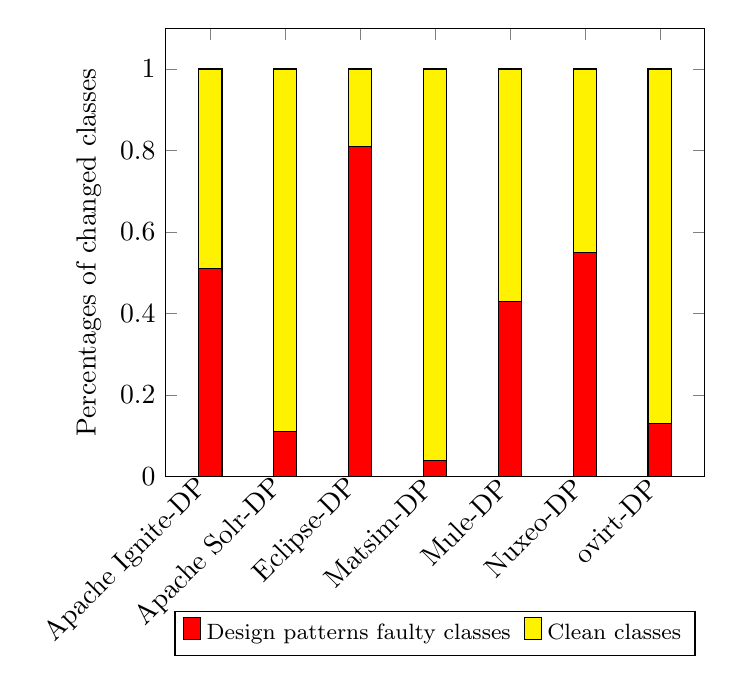
\begin{tikzpicture}
  \begin{axis}[
      every node near coord/.style={
     },
     legend style={
       font=\footnotesize,
       cells={anchor=east},
       legend columns=5,
       at={(0.50,-0.30)},
       anchor=north,
       /tikz/every even column/.append style={column sep=0.1cm}
     },
    title={},
    ybar stacked, ymin=0,
    bar width=3mm,
    ylabel={Percentages of changed classes},
    symbolic x coords=     {Apache Ignite-DP, Apache Solr-DP, Eclipse-DP, Matsim-DP, Mule-DP, Nuxeo-DP, ovirt-DP},
    xtick=data,
    x tick label style={rotate=45,anchor=east},
]
  %F
  \addplot [fill=red] coordinates {
%  ({Apache Ignite-AP},0.55)
  ({Apache Ignite-DP},0.51)
%  ({Apache Solr-AP},0.51)
  ({Apache Solr-DP},0.11)
%  ({Eclipse-AP},0.86)
  ({Eclipse-DP},0.81)
%  ({Matsim-AP},0.08)
  ({Matsim-DP},0.04)
%  ({Mule-AP},0.59)
  ({Mule-DP},0.43)
%  ({Nuxeo-AP},0.64)
  ({Nuxeo-DP},0.55)
%  ({Ovirt-AP},0.20)
  ({ovirt-DP},0.13)
};
    \addplot [fill=yellow] coordinates {
%  ({Apache Ignite-AP},0.45)
  ({Apache Ignite-DP},0.49)
%  ({Apache Solr-AP},0.49)
  ({Apache Solr-DP},0.89)
%  ({Eclipse-AP},0.14)
  ({Eclipse-DP},0.19)
%  ({Matsim-AP},0.92)
  ({Matsim-DP},0.96)
%  ({Mule-AP},0.41)
  ({Mule-DP},0.57)
%  ({Nuxeo-AP},0.36)
  ({Nuxeo-DP},0.45)
%  ({Ovirt-AP},0.80)
  ({ovirt-DP},0.87)
};
  \legend {Design patterns faulty classes, Clean classes} 
  \end{axis}
  \end{tikzpicture}
  }
 \caption{Faulty changed classes percentages with design pattern in the studied systems} 
\label{fig:DPFaultyChangedClasses}
\end{figure}

\begin{figure}[ht]
\centering
\scalebox{0.8}{
  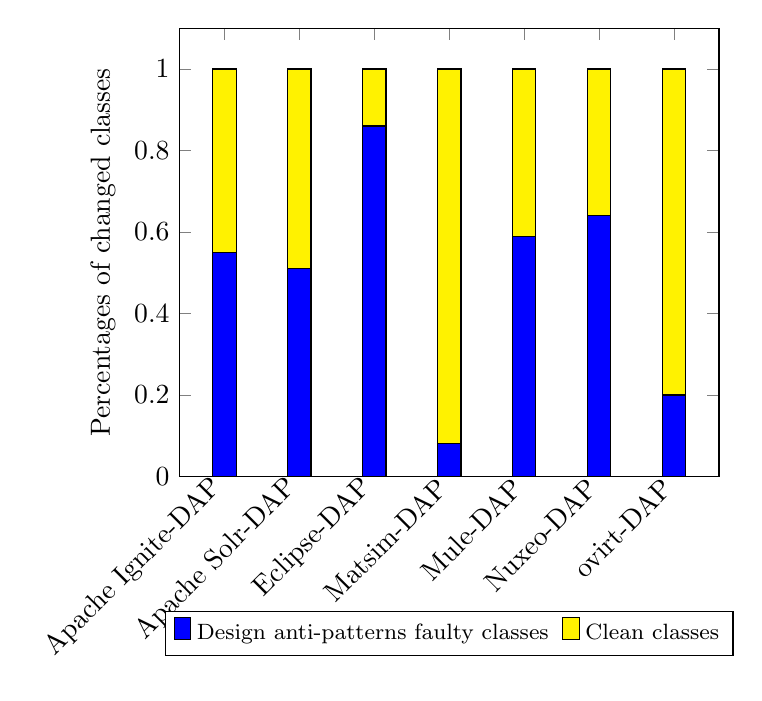
\begin{tikzpicture}
  \begin{axis}[
      every node near coord/.style={
     },
     legend style={
       font=\footnotesize,
       cells={anchor=east},
       legend columns=5,
       at={(0.50,-0.30)},
       anchor=north,
       /tikz/every even column/.append style={column sep=0.1cm}
     },
    title={},
    ybar stacked, ymin=0,
    bar width=3mm,
    ylabel={Percentages of changed classes},
    symbolic x coords=     {Apache Ignite-DAP, Apache Solr-DAP, Eclipse-DAP, Matsim-DAP, Mule-DAP, Nuxeo-DAP, ovirt-DAP},
    xtick=data,
    x tick label style={rotate=45,anchor=east},
]
  %F
  \addplot [fill=blue] coordinates {
  ({Apache Ignite-DAP},0.55)
%  ({Apache Ignite-DP},0.51)
  ({Apache Solr-DAP},0.51)
%  ({Apache Solr-DP},0.11)
  ({Eclipse-DAP},0.86)
%  ({Eclipse-DP},0.81)
  ({Matsim-DAP},0.08)
%  ({Matsim-DP},0.04)
  ({Mule-DAP},0.59)
%  ({Mule-DP},0.43)
  ({Nuxeo-DAP},0.64)
%  ({Nuxeo-DP},0.55)
  ({ovirt-DAP},0.20)
%  ({Ovirt-DP},0.13)
};

  \addplot [fill=yellow] coordinates {
  ({Apache Ignite-DAP},0.45)
%  ({Apache Ignite-DP},0.49)
  ({Apache Solr-DAP},0.49)
%  ({Apache Solr-DP},0.89)
  ({Eclipse-DAP},0.14)
%  ({Eclipse-DP},0.19)
  ({Matsim-DAP},0.92)
%  ({Matsim-DP},0.96)
  ({Mule-DAP},0.41)
%  ({Mule-DP},0.57)
  ({Nuxeo-DAP},0.36)
%  ({Nuxeo-DP},0.45)
  ({ovirt-DAP},0.80)
%  ({Ovirt-DP},0.87)
};
  \legend {Design anti-patterns faulty classes, Clean classes} 
  \end{axis}
  \end{tikzpicture}
  }
 \caption{Faulty changed classes with design anti-patterns percentages in the studied systems} 
\label{fig:APFaultyChangedClasses}
\end{figure}

\begin{figure}
\centering
\scalebox{1.1}{
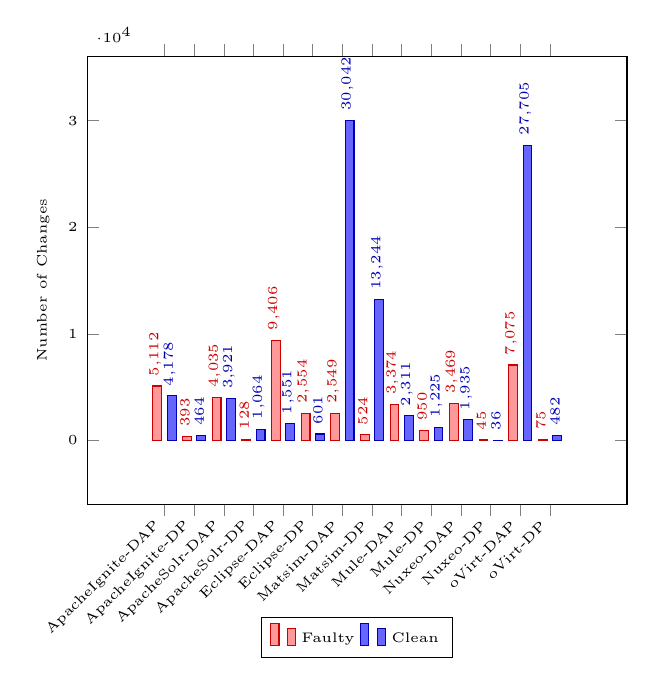
\begin{tikzpicture}
\pgfplotsset{every node/.append style={font=\tiny}}
\pgfplotsset{every tick label/.append style={font=\tiny}}
\begin{axis}[
    ybar,
    ymin=0,
    enlargelimits=0.2,
    legend style={at={(0.5,-0.25)},anchor=north,legend columns=-1},
    bar width=1.12mm,
    ylabel={Number of Changes},
    symbolic x coords={ApacheIgnite-DAP, ApacheIgnite-DP, ApacheSolr-DAP, ApacheSolr-DP, Eclipse-DAP, Eclipse-DP, Matsim-DAP, Matsim-DP, Mule-DAP, Mule-DP, Nuxeo-DAP, Nuxeo-DP, oVirt-DAP, oVirt-DP},
    xtick=data,
    x tick label style={rotate=45,anchor=east},
    nodes near coords,
    nodes near coords align={center},style={font=\tiny},
    every node near coord/.append style={rotate=90,anchor=south west,
    inner ysep=-1.75pt,}
    ]

\addplot [red!80!black,fill=red!40] coordinates {
(ApacheIgnite-DAP,5112) (ApacheIgnite-DP,393) (ApacheSolr-DAP,4035) (ApacheSolr-DP,128) (Eclipse-DAP,9406) (Eclipse-DP,2554) (Matsim-DAP,2549) (Matsim-DP,524) (Mule-DAP,3374) (Mule-DP,950) (Nuxeo-DAP,3469) (Nuxeo-DP,45) (oVirt-DAP,7075) (oVirt-DP,75)};
  
\addplot [blue!70!black,fill=blue!60] coordinates {
(ApacheIgnite-DAP,4178) (ApacheIgnite-DP,464) (ApacheSolr-DAP,3921) (ApacheSolr-DP,1064) (Eclipse-DAP,1551) (Eclipse-DP,601) (Matsim-DAP,30042) (Matsim-DP,13244) (Mule-DAP, 2311) (Mule-DP,1225) (Nuxeo-DAP,1935) (Nuxeo-DP,36) (oVirt-DAP,27705) (oVirt-DP,482)};
\legend{Faulty, Clean}
\end{axis}
\end{tikzpicture}
}
\caption{Faulty changed classes with design anti-patterns and design patterns in the studied systems} 
\label{fig:AP_DPFaultyChangedClasses}
\end{figure}

\begin{tcolorbox}
\vspace{-0.1cm}
\textbf{Summary:} \emph{Some change types applied to design patterns and design anti-patterns make software systems more fault-prone compared to others. We observed that, in all the studied systems, Renaming, Comment, and Operator are the change types from design patterns to design anti-patterns that most lead to faults.}
\vspace{-0.1cm}
\end{tcolorbox}
% !TEX root = Guillon2017_arxiv.tex

%% Short Recap

Graph analysis of brain networks have been largely exploited in the study of AD with the aim to extract new predictive diagnostics of disease progression.
Typical approaches in functional neuroimaging, characterized by oscillatory dynamics, analyze brain networks separately at different frequencies thus neglecting the available multivariate spectral information.
Here, we adopted a method to formally take into account the topological information of multi-frequency connectomes obtained from source-reconstructed MEG signals in a group of AD and healthy subjects during EC resting states.

%% Multiplex Results

Main results showed that, while flattening networks of different frequency bands attenuates differences between AD and HC populations, keeping the multiplex nature of MEG connectomes allow to capture higher-order discriminant information.
AD subjects exhibited an aberrant multiplex brain network structure that significantly reduced the global propensity to facilitate information propagation across frequency bands as compared to HC subjects (\autoref{fig:participation}b, inset). This could be in part explained by the higher variability of the individual node degrees across bands (\autoref{fig:coefficient_of_variation}).

% NOTE: High MPCi does not necessarily mean high oi (autoref fig:mpca) but it also seems that having a high number of connections (high oi) and a low MPC is not possible in the case of the brain.

% NOTE: In general, a ROI with a high MPC but with low oi, will have an even higher MPC if its oi increase (for another subject for instance). In clear: for a given i (i.e. a given ROI), the corrcoeff between oi and MPCi is always positive.

% NOTE: I tested different thresholds and with the ImCoh to check if it was not because of the week noisy connections, but the distribution of MPCi values seems to be always the same. Even with an average degree of 1 meaning that the brain always tends to keep connections in multiples frequency bands in the same time. Could it be explained by the fact that coherence is influenced by harmonics?

Such loss of inter-frequency centrality was mostly localized in association areas as well as in the cingulate cortex (\autoref{fig:participation}b; \autoref{tab:local_participation}), which resulted the most important hub promoting interaction across bands in the HC group (\autoref{fig:mpc}a).
Because all these areas are typically affected by AD atrophy \citep{wenk_neuropathologic_2003} we hypothesize that the anatomical withering might have impacted the neural oscillatory mechanisms supporting large-scale brain functional integration. Notably, the significant alteration of the connectivity across bands observed in the cingulate cortex could be ascribed to typical M/EEG connectivity changes observed in AD, such as reduced $alpha$ coherence \citep{stam_magnetoencephalographic_2006,jeong_eeg_2004,dauwels_diagnosis_2010,wang_power_2015} (\autoref{fig:mpc}b).
We also found a significant decrease in the primary motor cortex (right precentral gyrus). While previous studies have identified this specific region as a connector hub in human brain networks \citep{tijms_alzheimers_2013}, its role in AD still needs to be clarified in terms of node centrality's changes with respect to healthy conditions.
%For these affected ROIs the decreased centrality was reflected by fewer interactions with higher sensory rhythms ($>20$ Hz) \citep{basar_review_2013} and more connections to lower attentional ones ($<13$ Hz) \citep{klimesch_EEG_1999} (\autoref{fig:participation}c).

% Single-Layer Results
While flattening network layers represents in general an oversimplification, analyzing single layers can still be a valid approach that is worth of investigation.
Because the $MPC$ is a pure multiplex quantity, we considered the conceptually akin version for single-layer networks, the standard participation coefficient $PC$, which evaluates the tendency of nodes to integrate information from different modules, rather than from different layers \citep{guimera_cartography_2005, battiston_structural_2014}.
AD patients exhibited lower inter-modular connectivity in the \textit{gamma} band with respect to HC subjects (\autoref{fig:participation}a; \autoref{tab:local_participation}) that was localized in association areas including frontal, temporal, and parietal cortices (\autoref{fig:participation}a; \autoref{tab:local_participation}).
%
Damages to these regions can lead to deficits in attention, recognition and planning \citep{purves_neuroscience_2001}. Our results support the hypothesis that AD could include a disconnection syndrome  \citep{pearson_anatomical_1985,arnold_topographical_1991,catani_rises_2005}.
Furthermore, they are in line with previous findings showing $PC$ decrements in AD, although those declines were more evident in lower frequency bands and therefore ascribed to possible long-range low-frequency connectivity alteration \citep{de_haan_disrupted_2012,tijms_alzheimers_2013}.

%% Conclusion
Put together, our findings indicated that AD alters the global brain network organization through connection disruption in several association regions, which play important roles in sensory processing by integrating information from other cortical regions through high-frequency channels \citep{miltner_coherence_1999-1,buschman_top-down_2007, siegel_neuronal_2008, gregoriou_high-frequency_2009, hipp_oscillatory_2011}.
%
Notably, we showed that the global loss of inter-modular interactions in the \textit{gamma} band is paralleled by a diffused decrease of inter-frequency centrality.
Future studies, involving recordings of limbic structures and/or stimulation-based techniques, should elucidate whether these two distinct reorganizational processes are truly independent or linked through possible cross-frequency mechanisms which are known to be essential for normal memory formation \citep{canolty_high_2006,axmacher_cross-frequency_2010, goutagny_alterations_2013}.


%% Classification Results

As a confirmation of the complementary information carried out by the multi-layer approach, we reported an increased classification accuracy when combining the local $PC$ and $MPC$ features.
The observed diagnostic power is in line with previous accuracy values obtained with standard graph theoretic approaches (around $80\%$) but exhibits slightly higher sensitivity ($>90\%$), which is often desired to avoid false negatives \citep{li_discriminant_2012, wang_disrupted_2013, wee_enriched_2011, wee_identification_2012, horwitz_functional_2011}.
Other approaches should determine if and to what extent the use of more sophisticated machine learning algorithms, or the inclusion of basic connectivity features \citep{hutchison_network-based_2011, shao_prediction_2012, zhou_hierarchical_2011} and different imaging modalities \citep{dai_discriminative_2012}, can lead to higher classification performance and better diagnosis \citep{tijms_alzheimers_2013}.

%% Correlation With MMSE

Previous works have documented relationships between brain network properties and neuropsychological measurements in AD, suggesting a potential impact for monitoring disease progression and for the development of new therapies
\citep{de_haan_functional_2009,lo_diffusion_2010,sanz-arigita_loss_2010-1,shu_disrupted_2012,stam_small-world_2007,wang_disrupted_2013}.
This is especially true for the standard $PC$ which has exhibited stronger correlations and larger between-group differences \citep{tijms_alzheimers_2013}.
In line with this prediction, we also reported significant correlations between the MMSE cognitive scores and the $PC$ values of the AD patients in the \textit{gamma} band (\autoref{fig:correlations}a).
%
An even stronger correlation was found, however, for the global $MPC$ values and the TR scores (\autoref{fig:correlations}b, \autoref{tab:local_correlation}).
Recent studies suggest that TR scores could be more specific for AD \citep{grober_free_2010, velayudhan_review_2014} as compared to MMSE scores which could be biased by differences in years of education, lack of sensitivity to progressive changes occurring with AD, as well as fail in detecting impairment caused by focal lesions \citep{tombaugh_mini-mental_1992}.
Locally, the regions whose $MPC$ correlated with TR were part of the default-mode network (DMN) (\autoref{tab:local_correlation}), which is heavily involved in memory formation and retrieval \citep{buckner_brains_2008,sperling_functional_2010}. According to recent hypothesis, these areas are directly affected by atrophy and metabolism disruption, as well as amyloid-$\beta$ deposition \citep{buckner_molecular_2005, greicius_default-mode_2004}.
Put together, our results suggest that AD symptoms related to episodic memory losses could be determined by the lower capacity of strategic DMN association areas to let information flow across different frequency channels.

\subsection*{Methodological considerations}

We estimated brain networks by means of spectral coherence, a connectivity measure widely used in the electrophysiological literature because of its simplicity and relatively intuitive interpretation \citep{srinivasan_eeg_2007}.
While this measure is known to suffer from possible volume conduction effects, recent evidence showed that source reconstruction techniques, like the one we adopted here, could at least mitigate this bias \citep{schoffelen_source_2009} and generate connectivity patterns consistent within and between subjects \citep{colclough_how_2016}.
In a separate analysis, we used the imaginary coherence as a candidate alternative to eliminate volume conduction effects \citep{nolte_identifying_2004}. We demonstrated that while no significant between-group differences could be obtained in terms of $MPC$ (data not shown here), the spatial distribution of the $MPC$ values was very similar to that observed in the brain networks obtained with the spectral coherence, especially for the internal regions along the longitudinal fissure (\autoref{fig:mpc_imcoh}).

Differently from other multiplex network quantities, such as those based on paths and walks \citep{boccaletti_structure_2014}, the $MPC$ has the advantage to not depend on the weights of the inter-layer links which, in general, are difficult to estimate or to assign from empirically obtained biological data. This is especially true in network neuroscience where, so far, the strength of the inter-layer connections is parametric and subject to arbitrariness \citep{de_domenico_mapping_2016} or estimated through measures of cross-frequency coupling \citep{brookes_multi-layer_2016-1} whose biological interpretation remains still to be completely elucidated \citep{jirsa_cross-frequency_2013}.

\section{Threats to Validity}
\label{sec:Treats to Validity}

We now discuss potential threats to the validity of the results of our study, following existing guidelines \cite{yin2013case,wohlin2012experimentation}.


\paragraph{Construct validity} These threats concern the relation between theory and observation. We know that the used design pattern and design anti-pattern detection techniques (DECOR and DeMIMA) in this study include some subjective understanding related to the definition of design patterns and design anti-patterns. Their authors reported recall rates of 100$\%$ for both techniques while the precision in the worst case was 31$\%$. We accept that the precision of these techniques is a concern. Some false positive classes may pass the validation because they ``looks like'' playing a role in some patterns.

We also accept that, in finding change types which led to faults, we could have matched classes that are not representing the actual same class. For example, class \texttt{C} is not match with \texttt{a.b.C.java} but could be matched with the \texttt{b.c.java}. Moreover, we know that during evolution, class names change as well. As for precision, the manual validation could be affected by subjectiveness or human error.  We should consider each type of renaming as we may misinterpret that there is a mutation between design patterns and design anti-patterns, while in fact the class name changed and the patterns remained stable. 



\paragraph{Internal validity} This threat concerns factors affecting our results. This threat is about the causality drawn from the study. It concerns our selection of studied systems and methodology. The accuracy of DECOR and DeMIMA impacts our results, because the number of design patterns and design anti-patterns computed with DECOR and DeMIMA is used to calculate the probabilities of mutations. Other detection techniques should be used to validate our findings.

Our results show correlations between design anti-patterns and design patterns, their mutations, and faults. However, they do not show causation. Hence, it is possible that some of the changes, which led to mutations, \eg{} changes to comments, although correlated to mutations, are not the root causes of these mutations. Identifying these root causes would require studying each change leading to mutations individually, manually, which is future work.



\paragraph{Conclusion validity} These threats concern the relationship between the treatment and the results. We paid attention in choosing the systems.

We used the SZZ algorithm \cite{sliwerski2005changes} to identify commits introducing faults. Although this algorithm may yield false positive results, it has been successfully employed in previous works, such as \cite{kamei2013large,fukushima2014empirical}. In this paper, to increase the algorithm's accuracy, we removed all fault-inducing commit candidates that only changed blank or comment lines. Moreover, the static analysis tool, srcML, can identify about 100 types of code elements from source code.

To make our results more actionable for software practitioners, we manually grouped similar element tags into 12 major change types as shown in Table~\ref{tab:Change_types}, which can help developers carefully change and review fault-prone code.



\paragraph{Reliability Validity} These threats concern the possibility of replicating the study. We provide all the necessary data on-line\footnote{\url{http://www.ptidej.net/downloads/replications/emse19c/}} to help other researchers replicate our work.



\paragraph{External validity} These threats concern the ability to generalize our results. We studied seven software systems with different sizes, domains, and complexity. We selected only Java systems because of the tools. We also chose some of these systems because they have been used in previous studies. Their numbers of lines of code range from hundred of thousands to several millions. These systems are widely used and have active developers community. They have several years of evolution histories. They are available on-line. However, all of them are written in Java and are open source. In the future, we plan to investigate more diverse set of systems. Moreover, we also want to study larger projects, with other programming languages, such as C++. 

We analysed commits instead of releases to cover as much as possible the whole histories of these systems. We choose thirteen design anti-patterns and eight design patterns among the many available patterns.
\section{Conclusion}
\label{sec:conclusion}
This paper presents a generic top-$\size$ recommendation framework for  trading-off accuracy, novelty, and coverage. To achieve this, we profile the users according to their preference for long-tail novelty. We examine various measures, and formulate an optimization problem to learn these user preferences from interaction data.  We then integrate the user preference estimates in our generic framework, GANC.  Extensive experiments on several datasets confirm that there are trade-offs between accuracy, coverage, and novelty. Almost all re-ranking models increase coverage and novelty at the cost of accuracy. However, existing re-ranking models typically rely on rating prediction models, and are hence more effective in dense settings. Using a generic approach, we can easily incorporate a suitable base accuracy recommender to devise an effective solution for both sparse and dense settings.  %Our results  also indicate there is no single method that outperforms other methods in all metrics. However our techniques obtain a significant improvement in coverage, while  . 
Although we integrated the  long-tail novelty preference estimates into a re-ranking framework, their use-case is not limited to these frameworks. In  the future, we intend to explore the temporal and topical dynamics of long-tail novelty preference, particularly in settings where contextual information is  available.  
%We achieve these objectives without using any additional contextual information.


\iffalse
While we focused on promoting long-tail items across users, we did not consider diversity of individual top-$\size$ recommendations, a factor that has been shown to positively affect consumer satisfaction. This is one direction for future work. Moreover, the sequential setting  in our work, creates a dependency between different batches, where,  the items recommended to a batch of users, depends on those recommended to previous batches. This dependency is created through the parameter $\mathbf{f}$, that is updated every time a top-$\size$ set  is allocated to a batch of users. A future direction for our work is to estimate a distribution over $\mathbf{f}$ that allows us to independently solve the problem for each user, leading to improvements across all performance metrics, including recommendation time. 

We design algorithms that take advantage of the structure in the value functions to obtain both efficient and scalable solutions. 
We design an algorithm that takes advantage of the structure in the value functions to obtain both efficient and scalable solutions. 

\textcolor{red}{Our  sequential  algorithms can be applied for batch recommendation contexts,~e.g., personalized email marketing, where based on prior interaction data between users and items,  a new round of recommendations must be sent to all users in the system.  However, the independent coverage algorithms lift the sequential setting restrictions and allow it be applied for re-ranking the output of base recommender in any setting. }A future direction for our work is to incorporate explicit diversity metrics in the framework. 
\fi


%We have a presented a submodular maximization framework to systematically trade-off relevance and diversity in recommendations to individual users and coverage across the item-space. This ensures both consumer and producer satisfaction. We model users according to their risk and focusing degrees and promote long-tail items to the right group of consumers. Consequently, we obtain a significant improvement in coverage while maintaining reasonable levels of user satisfaction. Furthermore, our methods are able to achieve a more balanced distribution across the set of recommended items. In the future, we plan to investigate the effect of using alternative base recommender systems. 

%Future Work
%However most of these methods assume that the ratings are missing at random (MAR). Since our method of generating recommendations is based on the completed matrix, assuming MAR might introduce additional bias, we will use methods which assume that the ratings at missing not at random (MNAR),explored in~\cite{steck2010training, icml2014c2_hernandez-lobatob14}. 	 
%Long Tail %Recently, authors in~\cite{cremonesi2010performance} conducted extensive experiments to evaluate the performances of various matrix factorization-based algorithms and neighborhood models on the task of recommending long tail items. Their experimental results show that long tail recommendation leads to a decrease in accuracy for all algorithms. They also showed that for this task, SVD outperforms other state-of-the-art algorithms. 




\balance
\newcommand{\student}[1]{#1}
\newcommand{\uml}{UML}
\bibliographystyle{IEEEtran} \scriptsize
\def\IEEEbibitemsep{0pt}
\bibliography{BibiTex}

\end{document}